% !TEX root = ../main.tex
%
\section{Performance of the measurement of the gluon-gluon fusion CP mixing angle}

\subsection{Prefit distributions for MELA approach}\label{prefit_mela_supp}

\begin{figure}[h!]
    \centering
        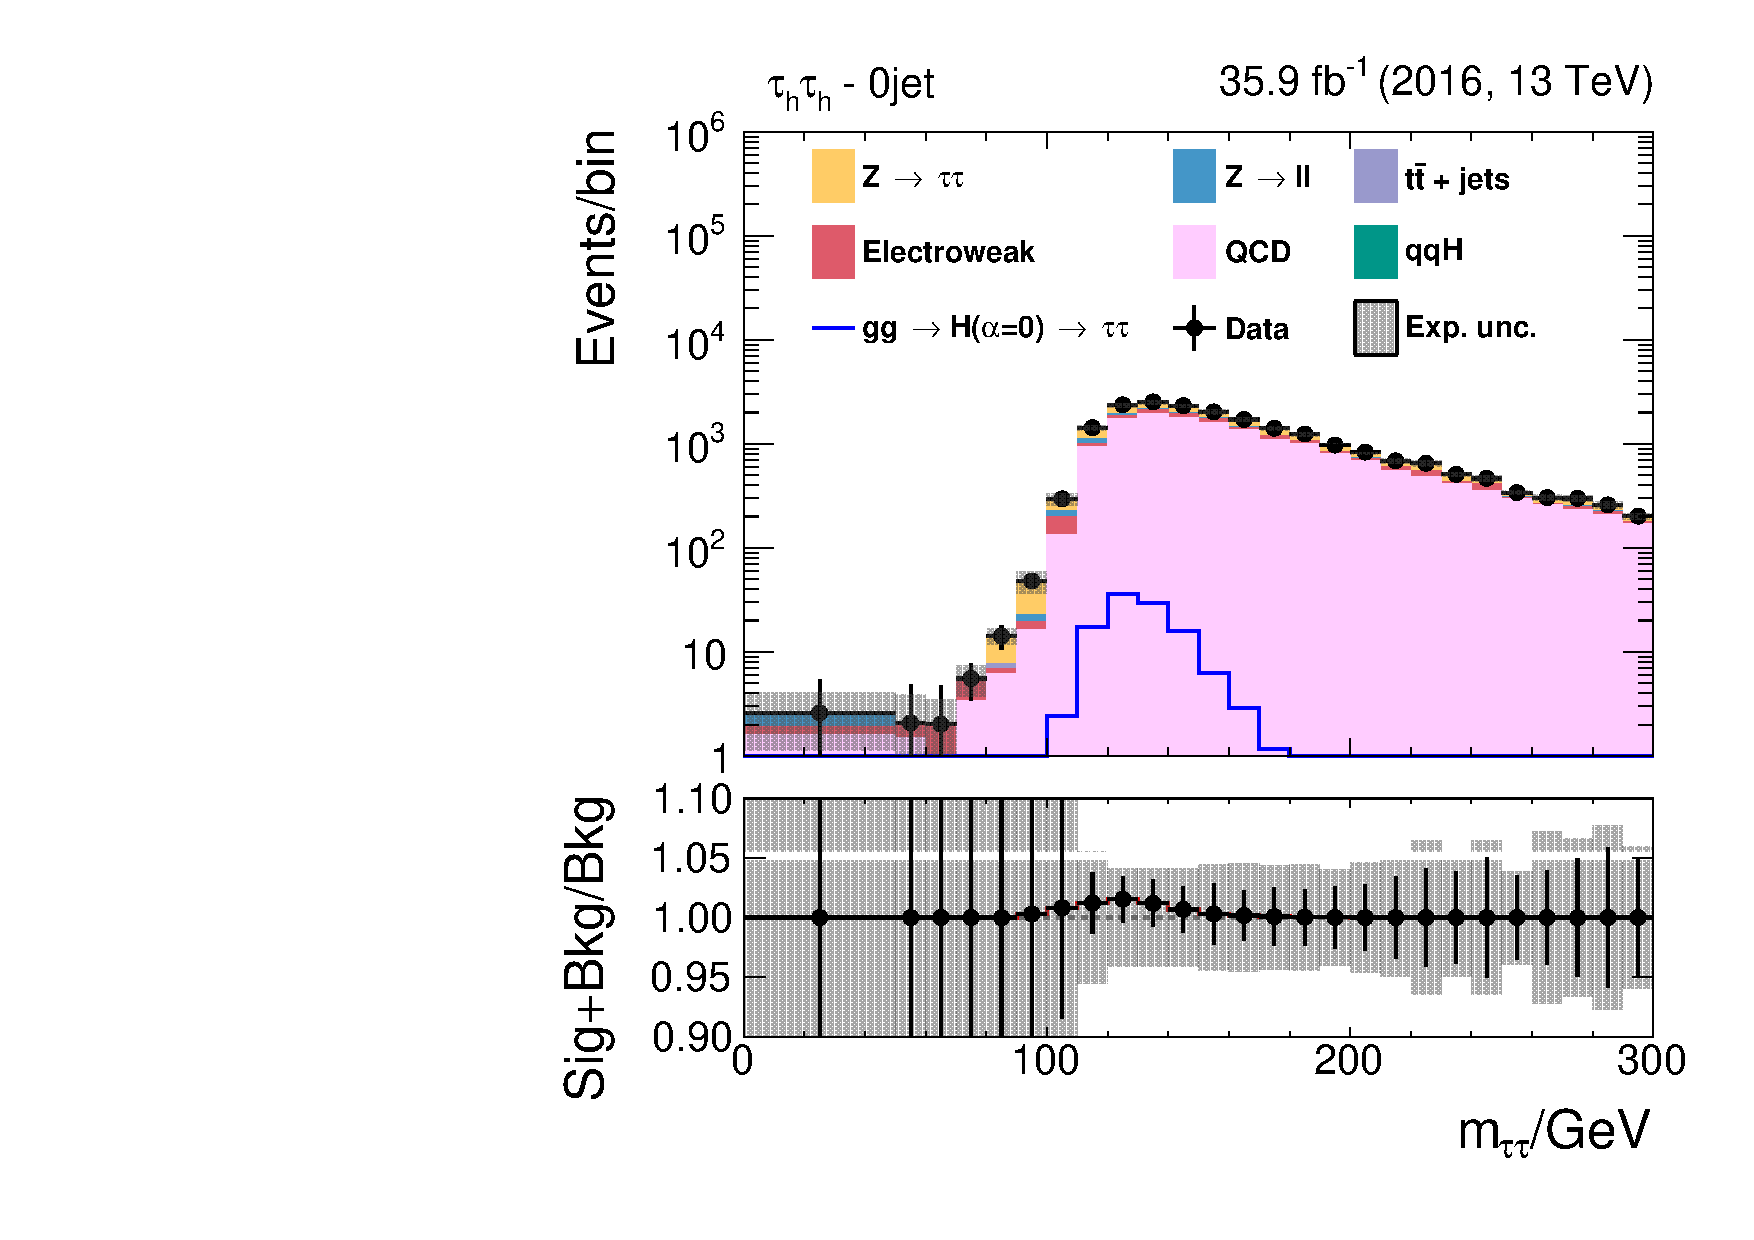
\includegraphics[width=.5\textwidth]{Figures/statana/Postfit_JEC_mela3D/prefit_htt_tt_1_13TeV.pdf}\\
        \includegraphics[width=\textwidth]{Figures/statana/Postfit_JEC_mela3D/prefit_htt_tt_2_13TeV.pdf}
        \caption{Prefit distributions of the \textit{0-jet} and \textit{boosted} categories in the \tautau{} channel using the MELA approach.}
    \end{figure}
\begin{figure}[h!]
        \centering
        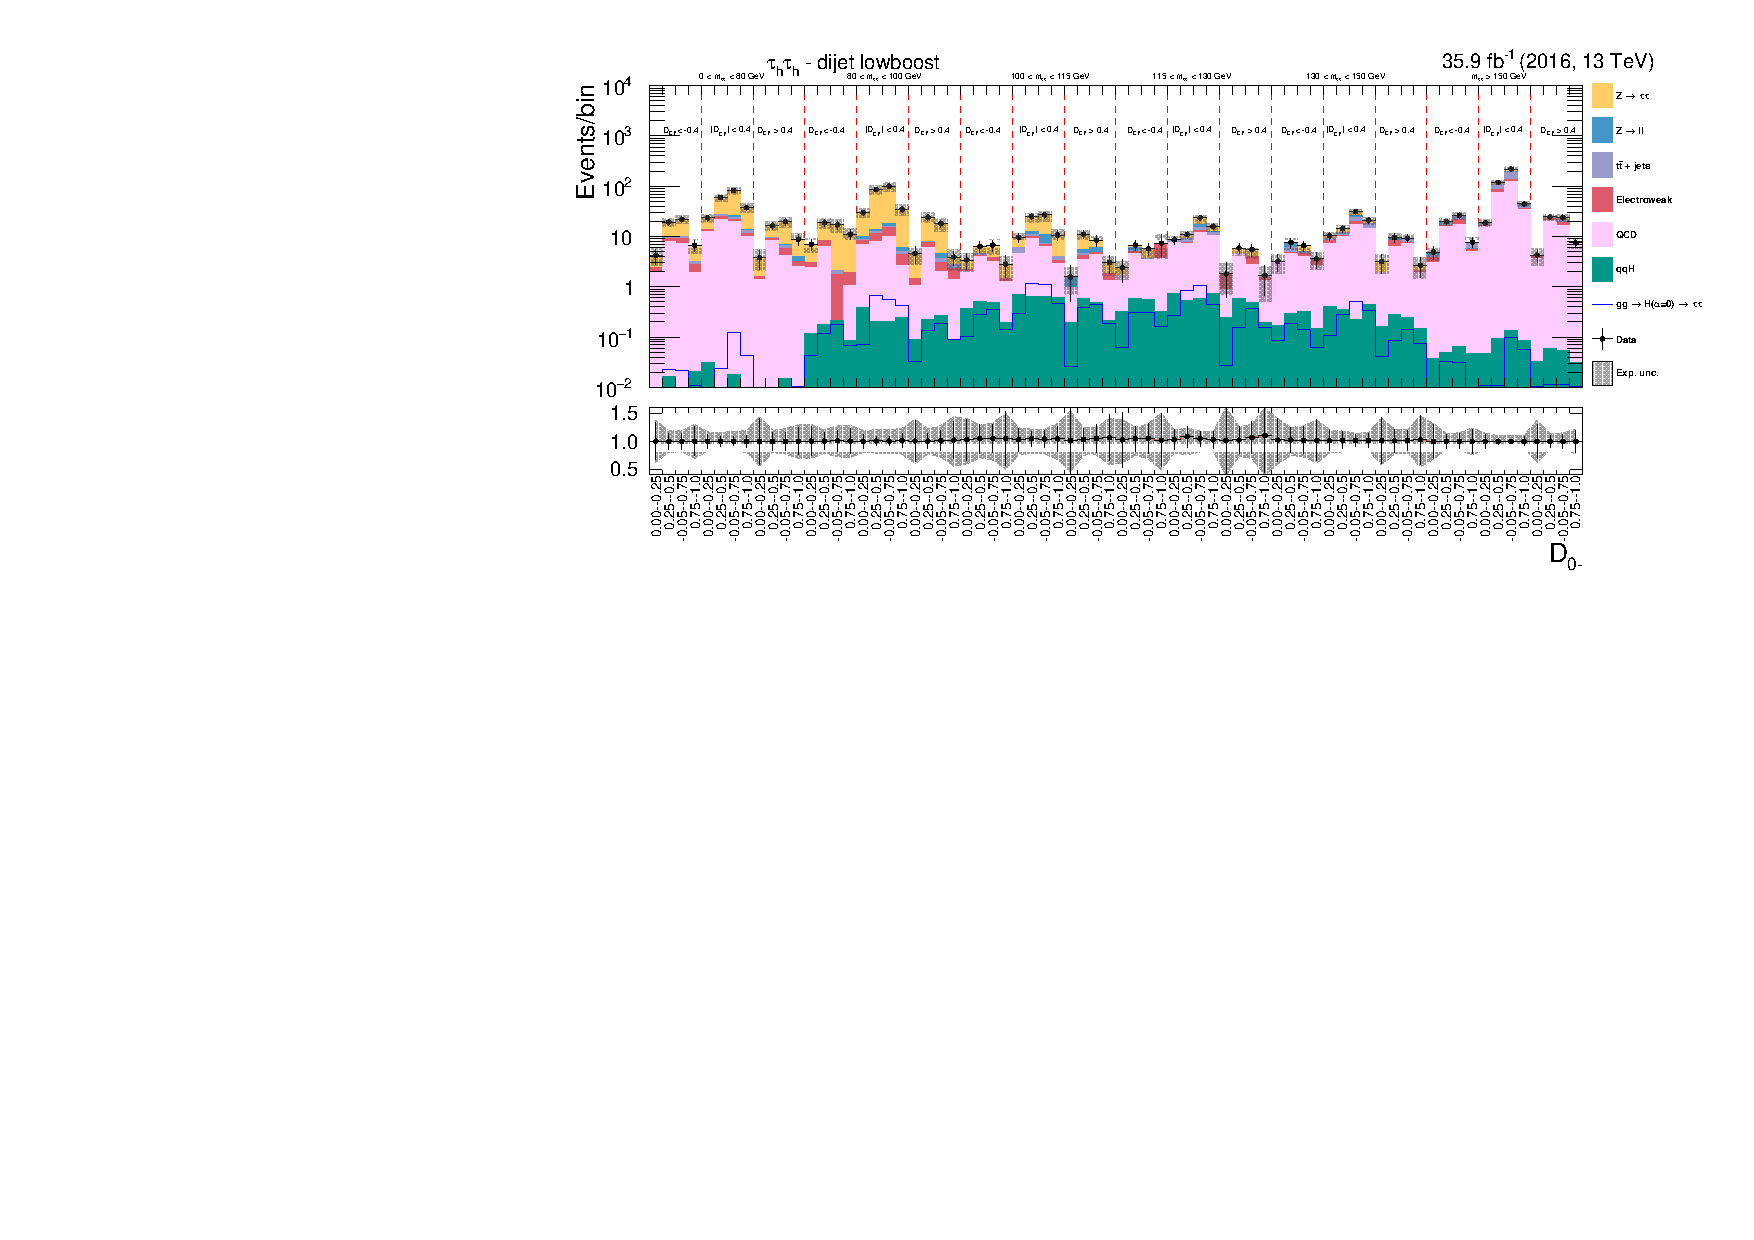
\includegraphics[width=\textwidth]{Figures/statana/Postfit_JEC_mela3D/prefit_htt_tt_3_13TeV.pdf}\\
        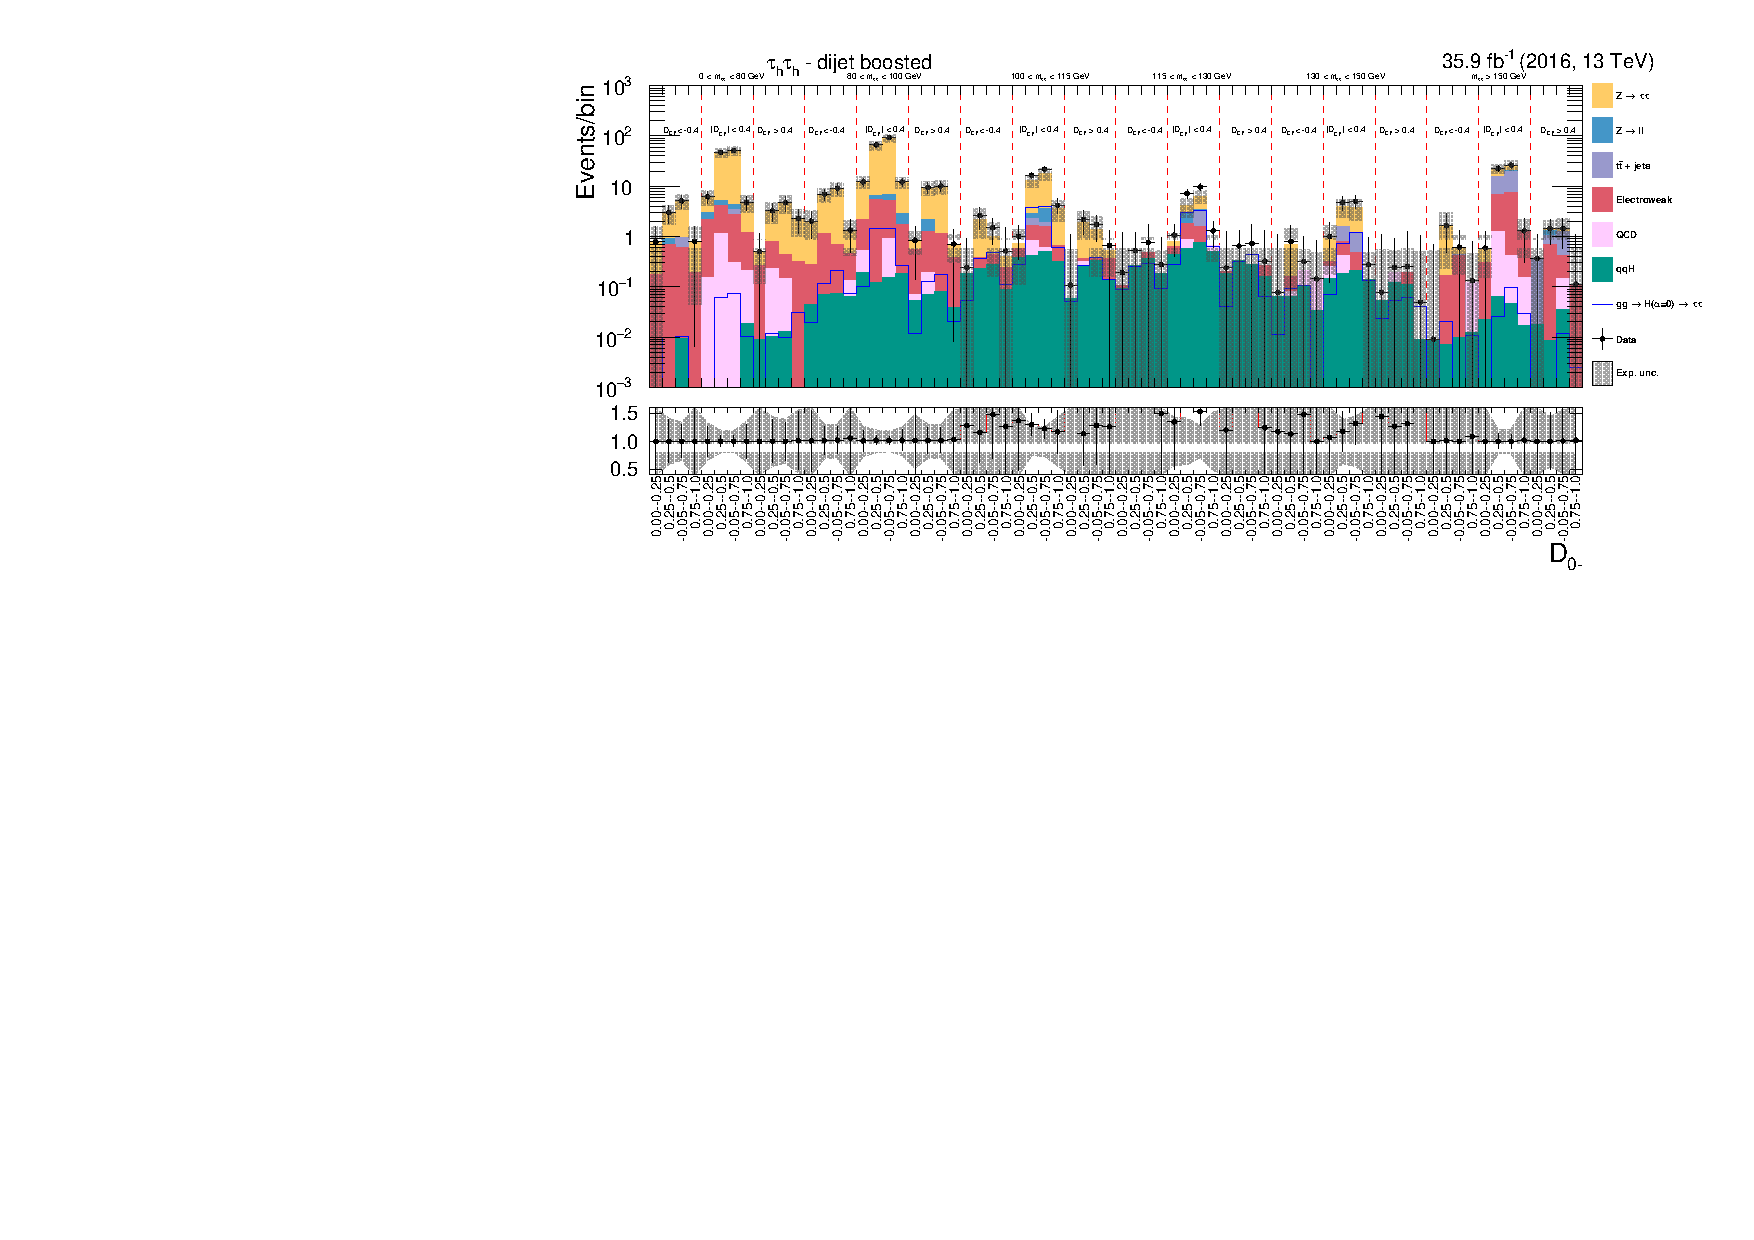
\includegraphics[width=\textwidth]{Figures/statana/Postfit_JEC_mela3D/prefit_htt_tt_4_13TeV.pdf}         
    \caption{Prefit distributions of the \textit{dijet lowboost} and \textit{dijet boosted} categories in the \tautau{} channel  using the MELA approach.}
\end{figure}
\clearpage
\begin{figure}[h!]
    \centering
        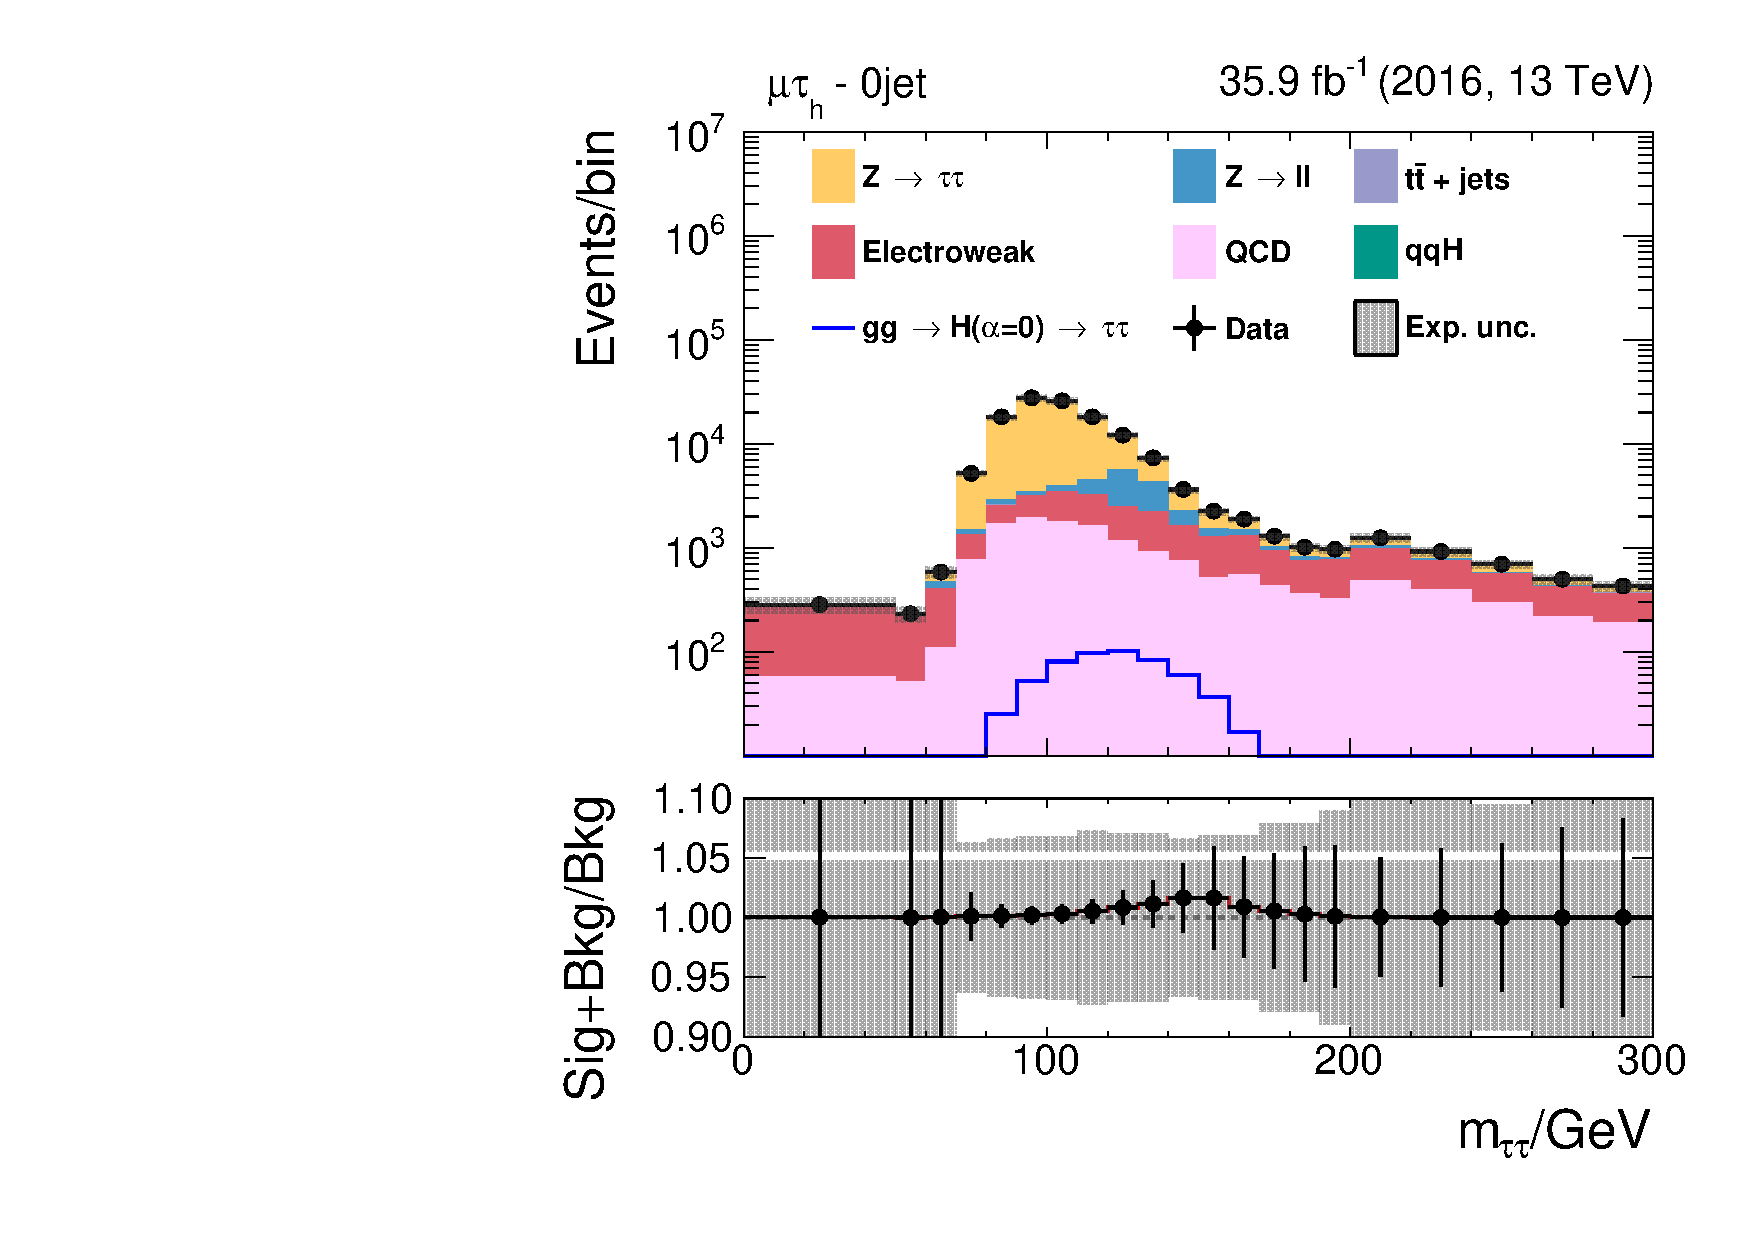
\includegraphics[width=.5\textwidth]{Figures/statana/Postfit_JEC_mela3D/prefit_htt_mt_1_13TeV.pdf}\\
        \includegraphics[width=\textwidth]{Figures/statana/Postfit_JEC_mela3D/prefit_htt_mt_2_13TeV.pdf}
        \caption{Prefit distributions of the \textit{0-jet} and \textit{boosted} categories in the \mutau{} channel using the MELA approach.}
    \end{figure}
    \begin{figure}[h!]
        \centering        
        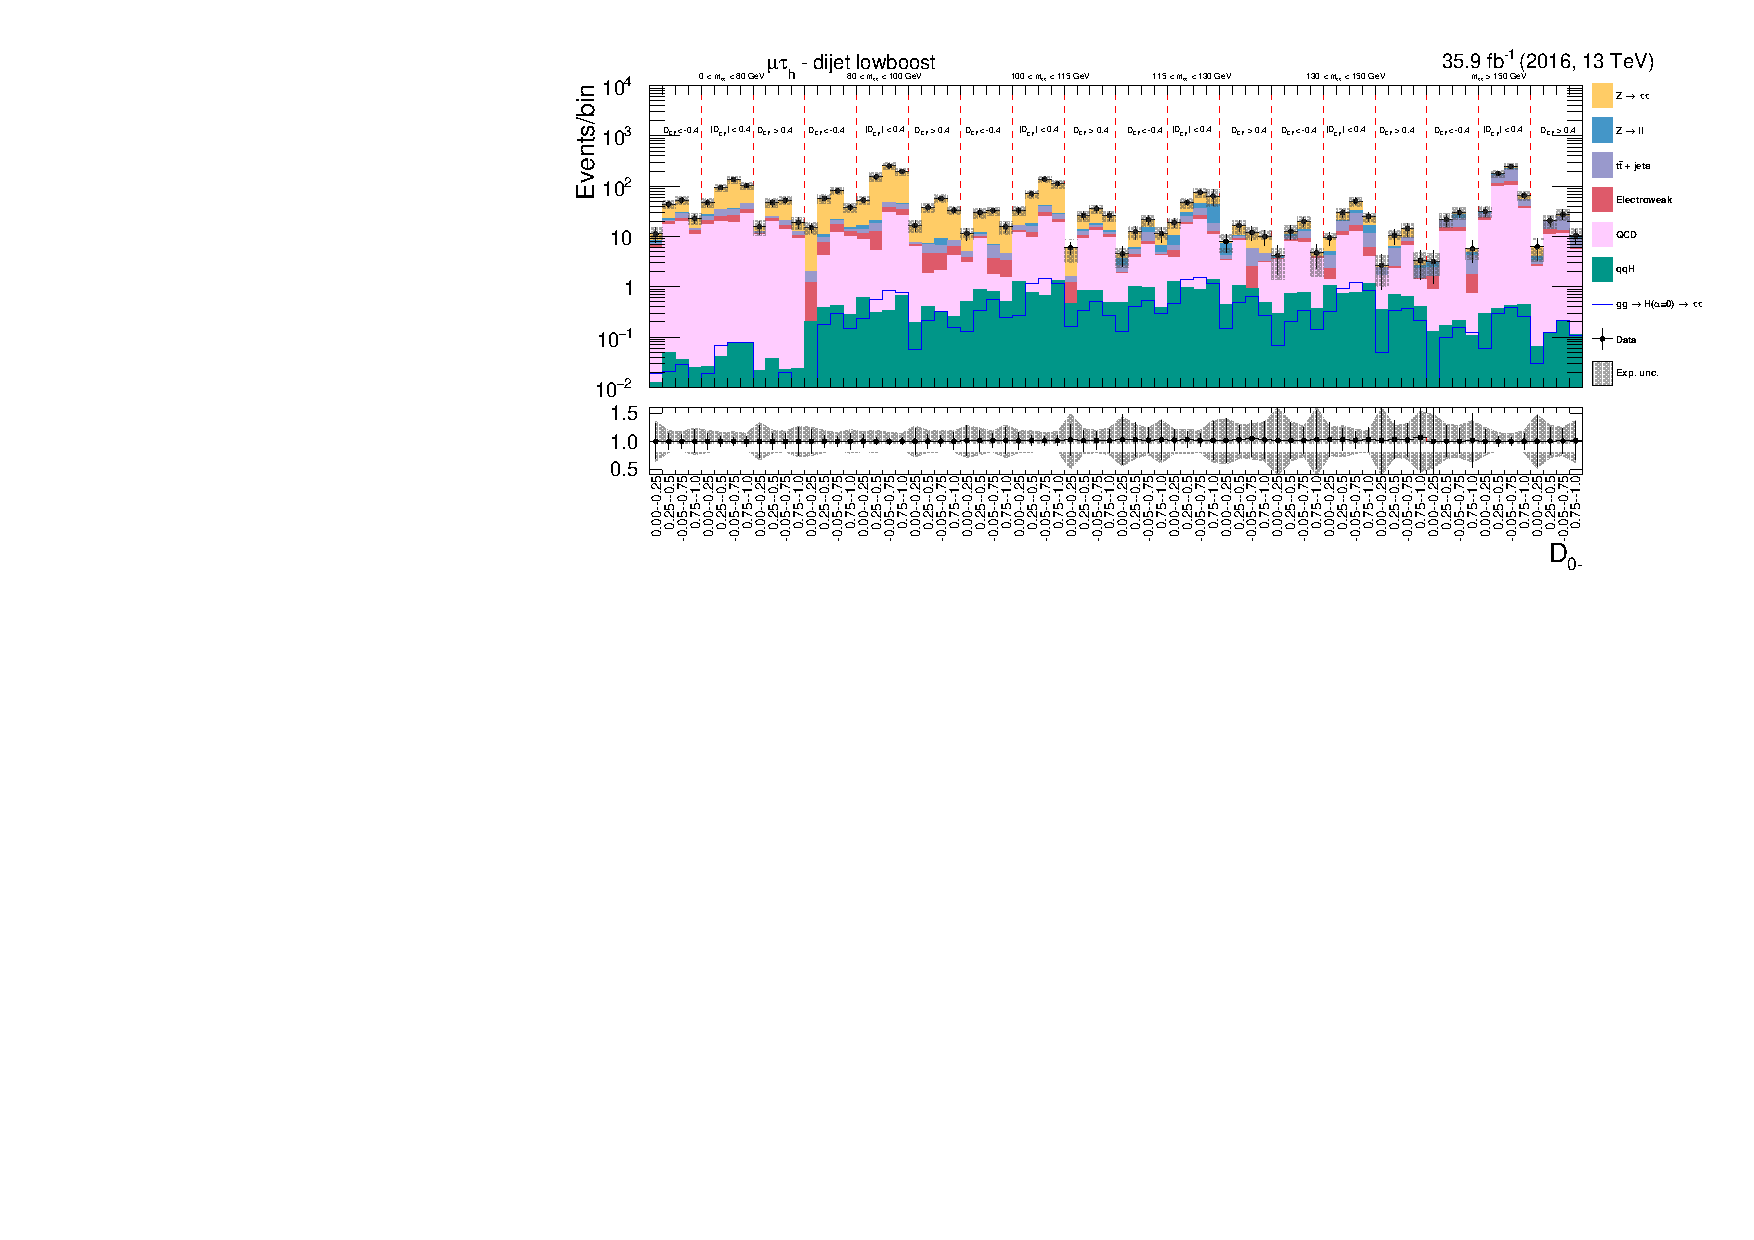
\includegraphics[width=\textwidth]{Figures/statana/Postfit_JEC_mela3D/prefit_htt_mt_3_13TeV.pdf}\\
        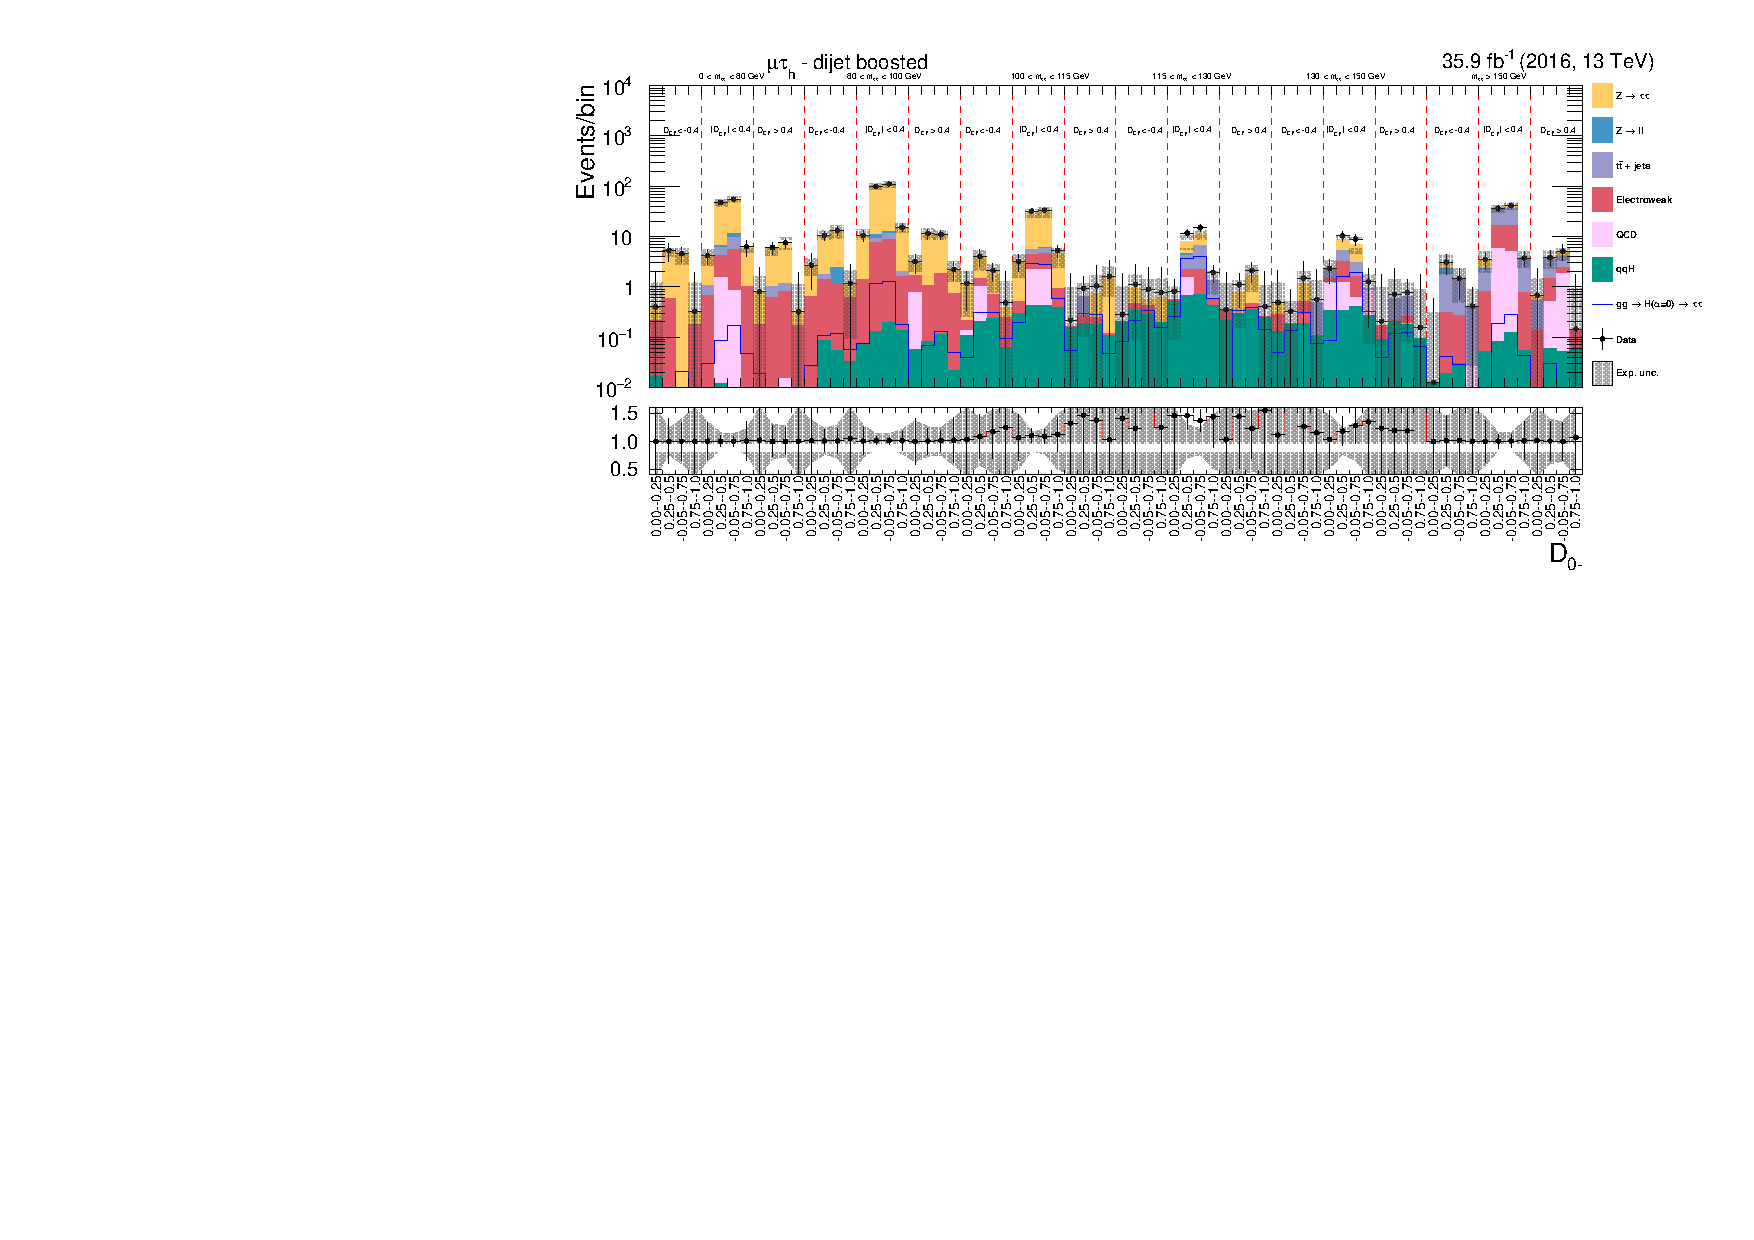
\includegraphics[width=\textwidth]{Figures/statana/Postfit_JEC_mela3D/prefit_htt_mt_4_13TeV.pdf}
    \caption{Prefit distributions of the \textit{dijet lowboost} and \textit{dijet boosted} categories in the \mutau{} channel  using the MELA approach.}
\end{figure}
\clearpage
\begin{figure}[h!]
    \centering
        \includegraphics[width=.5\textwidth]{Figures/statana/Postfit_JEC_mela3D/prefit_htt_et_1_13TeV.pdf}\\
        \includegraphics[width=\textwidth]{Figures/statana/Postfit_JEC_mela3D/prefit_htt_et_2_13TeV.pdf}
    \caption{Prefit distributions of the \textit{0-jet} and \textit{boosted} categories in the \etau{} channel  using the MELA approach.}
\end{figure}  
\begin{figure}[h!]
    \centering      
        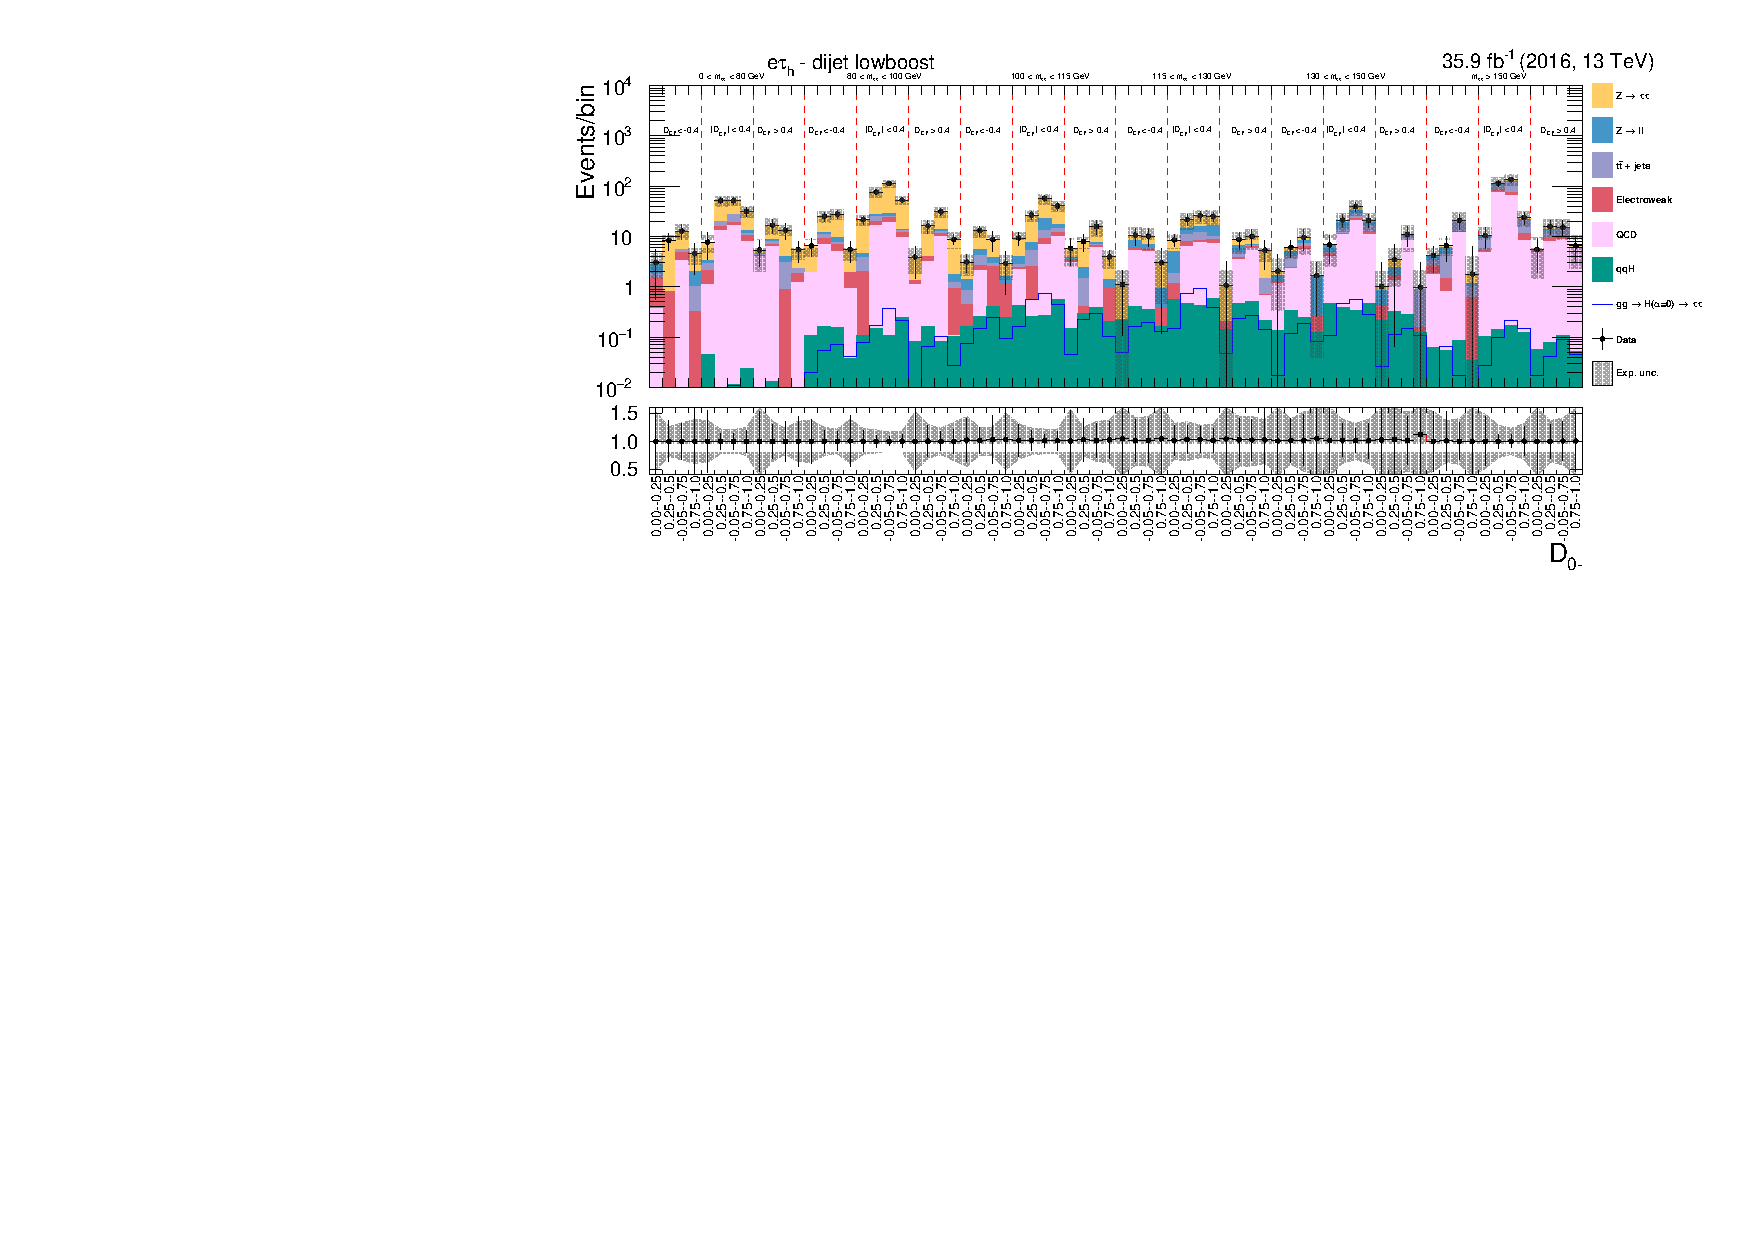
\includegraphics[width=\textwidth]{Figures/statana/Postfit_JEC_mela3D/prefit_htt_et_3_13TeV.pdf}\\
        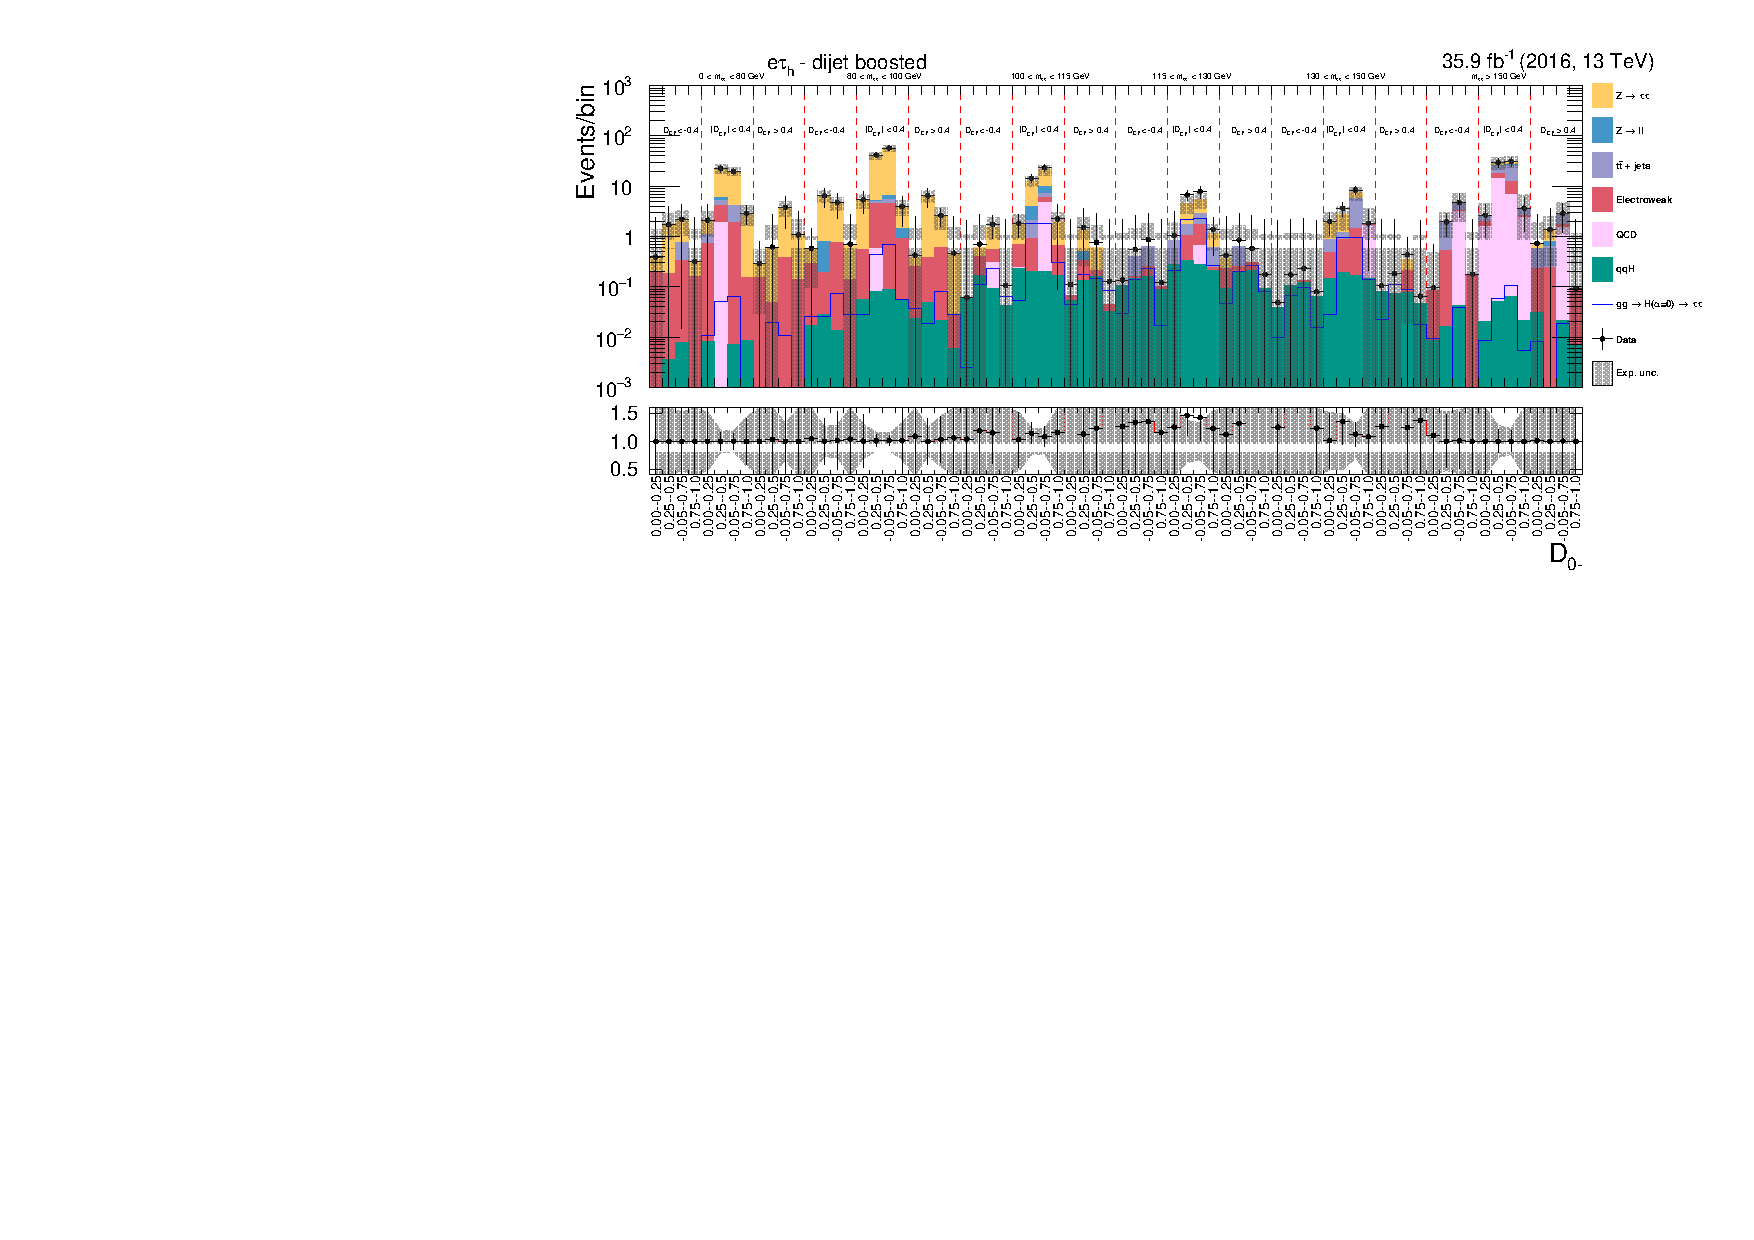
\includegraphics[width=\textwidth]{Figures/statana/Postfit_JEC_mela3D/prefit_htt_et_4_13TeV.pdf}
    \caption{Prefit distributions of the \textit{dijet lowboost} and \textit{dijet boosted} categories in the \etau{} channel  using the MELA approach.}
\end{figure}
\clearpage
\begin{figure}[h!]
    \centering
        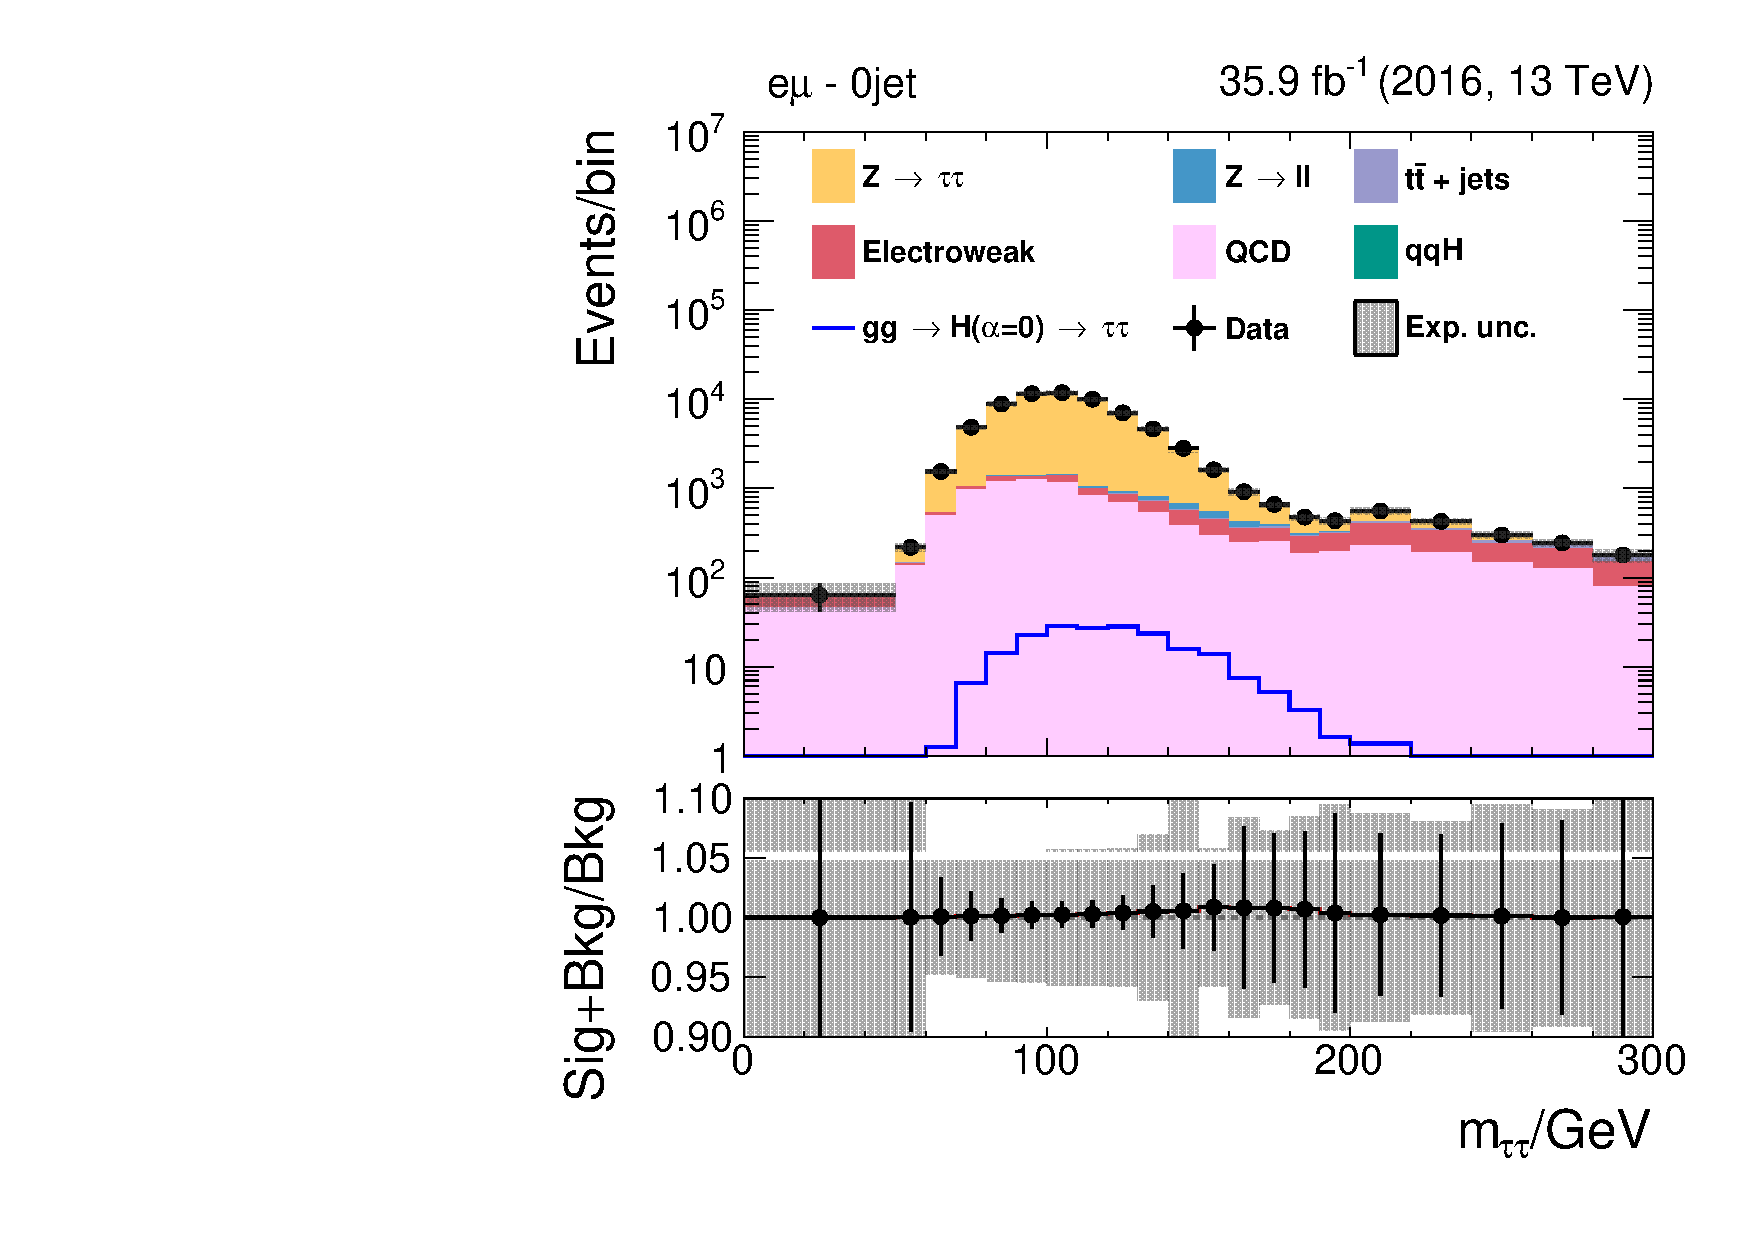
\includegraphics[width=.5\textwidth]{Figures/statana/Postfit_JEC_mela3D/prefit_htt_em_1_13TeV.pdf}\\
        \includegraphics[width=\textwidth]{Figures/statana/Postfit_JEC_mela3D/prefit_htt_em_2_13TeV.pdf}
    \caption{Prefit distributions of the \textit{0-jet} and \textit{boosted} categories in the \emu{} channel  using the MELA approach.}
\end{figure} 
\begin{figure}[h!]
    \centering       
        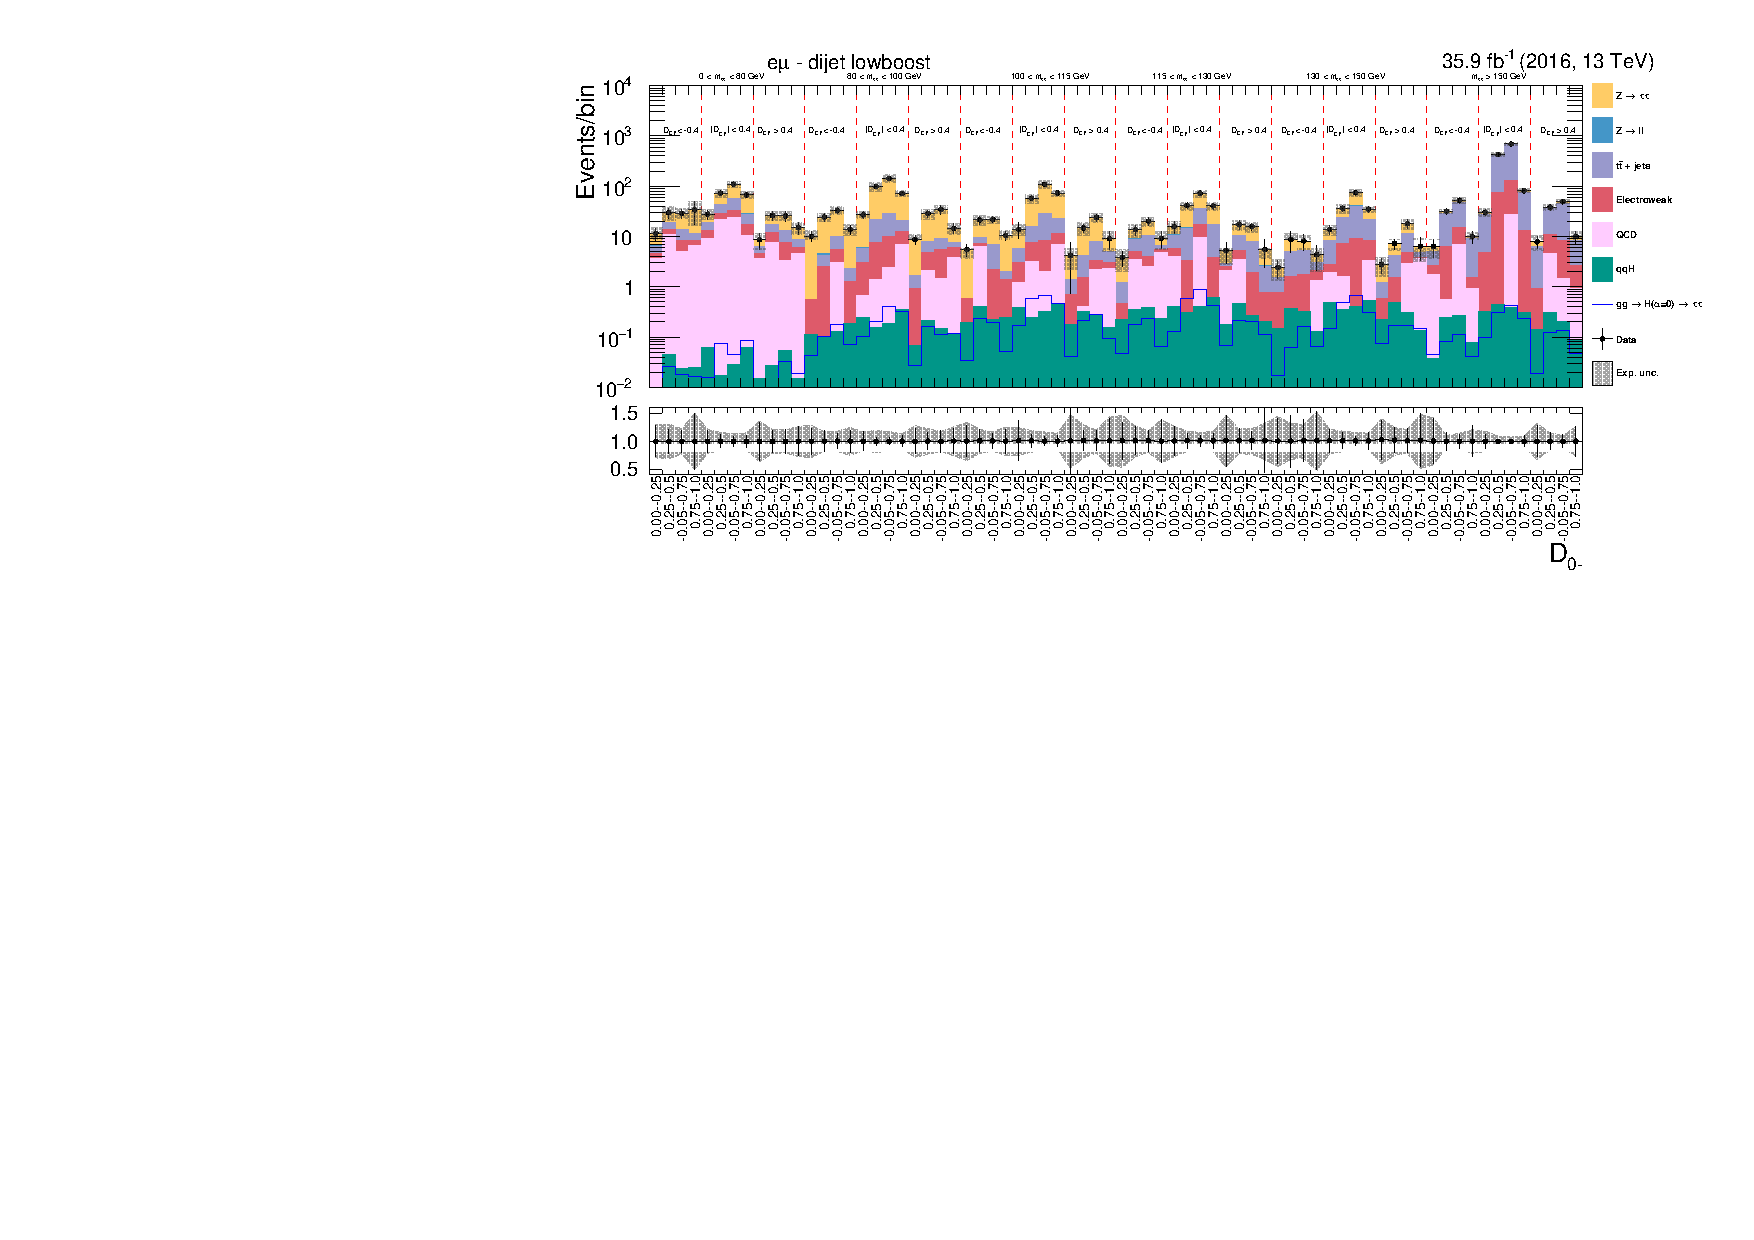
\includegraphics[width=\textwidth]{Figures/statana/Postfit_JEC_mela3D/prefit_htt_em_3_13TeV.pdf}\\
        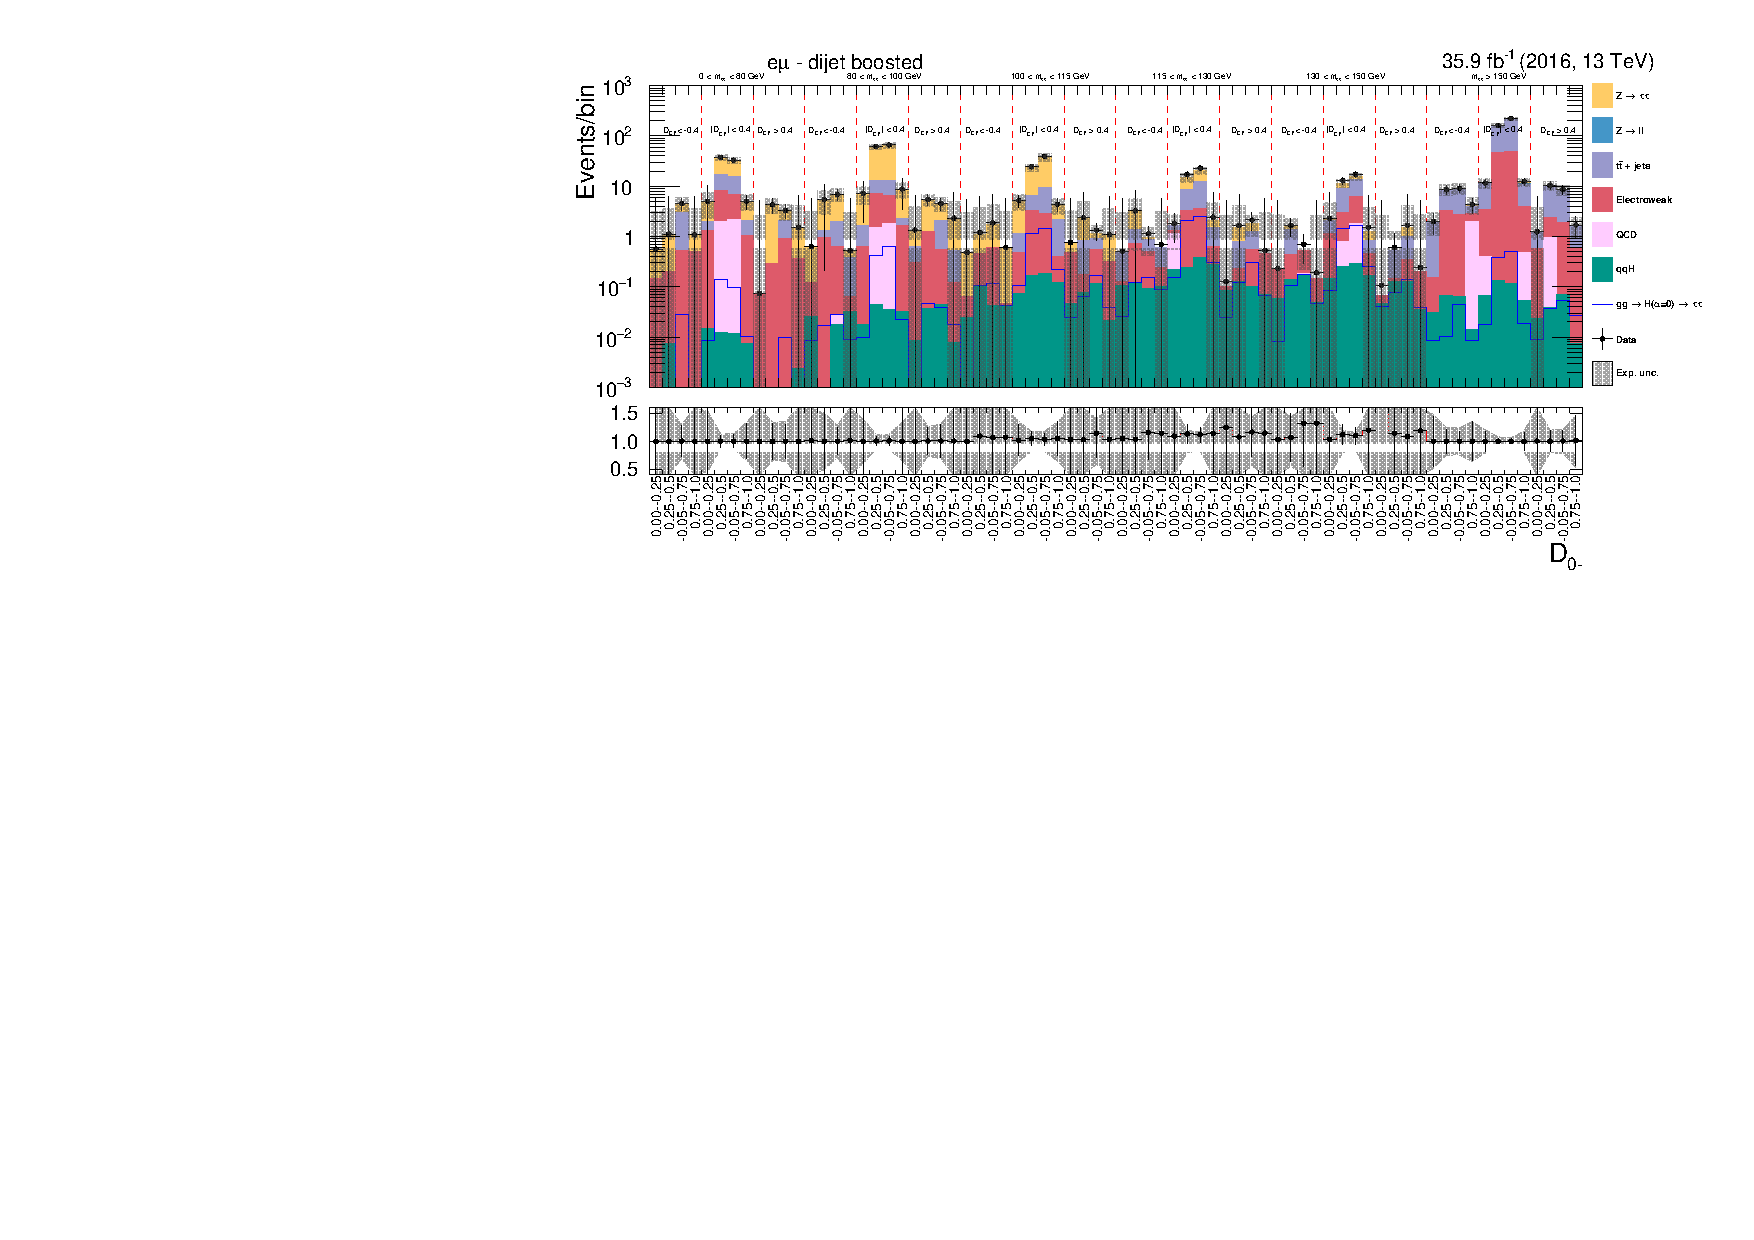
\includegraphics[width=\textwidth]{Figures/statana/Postfit_JEC_mela3D/prefit_htt_em_4_13TeV.pdf}
    \caption{Prefit distributions of the \textit{dijet lowboost} and \textit{dijet boosted} categories in the \emu{} channel  using the MELA approach.}
\end{figure}
\clearpage
\subsection{Postfit distributions for MELA approach}

\begin{figure}[h!]
    \centering
        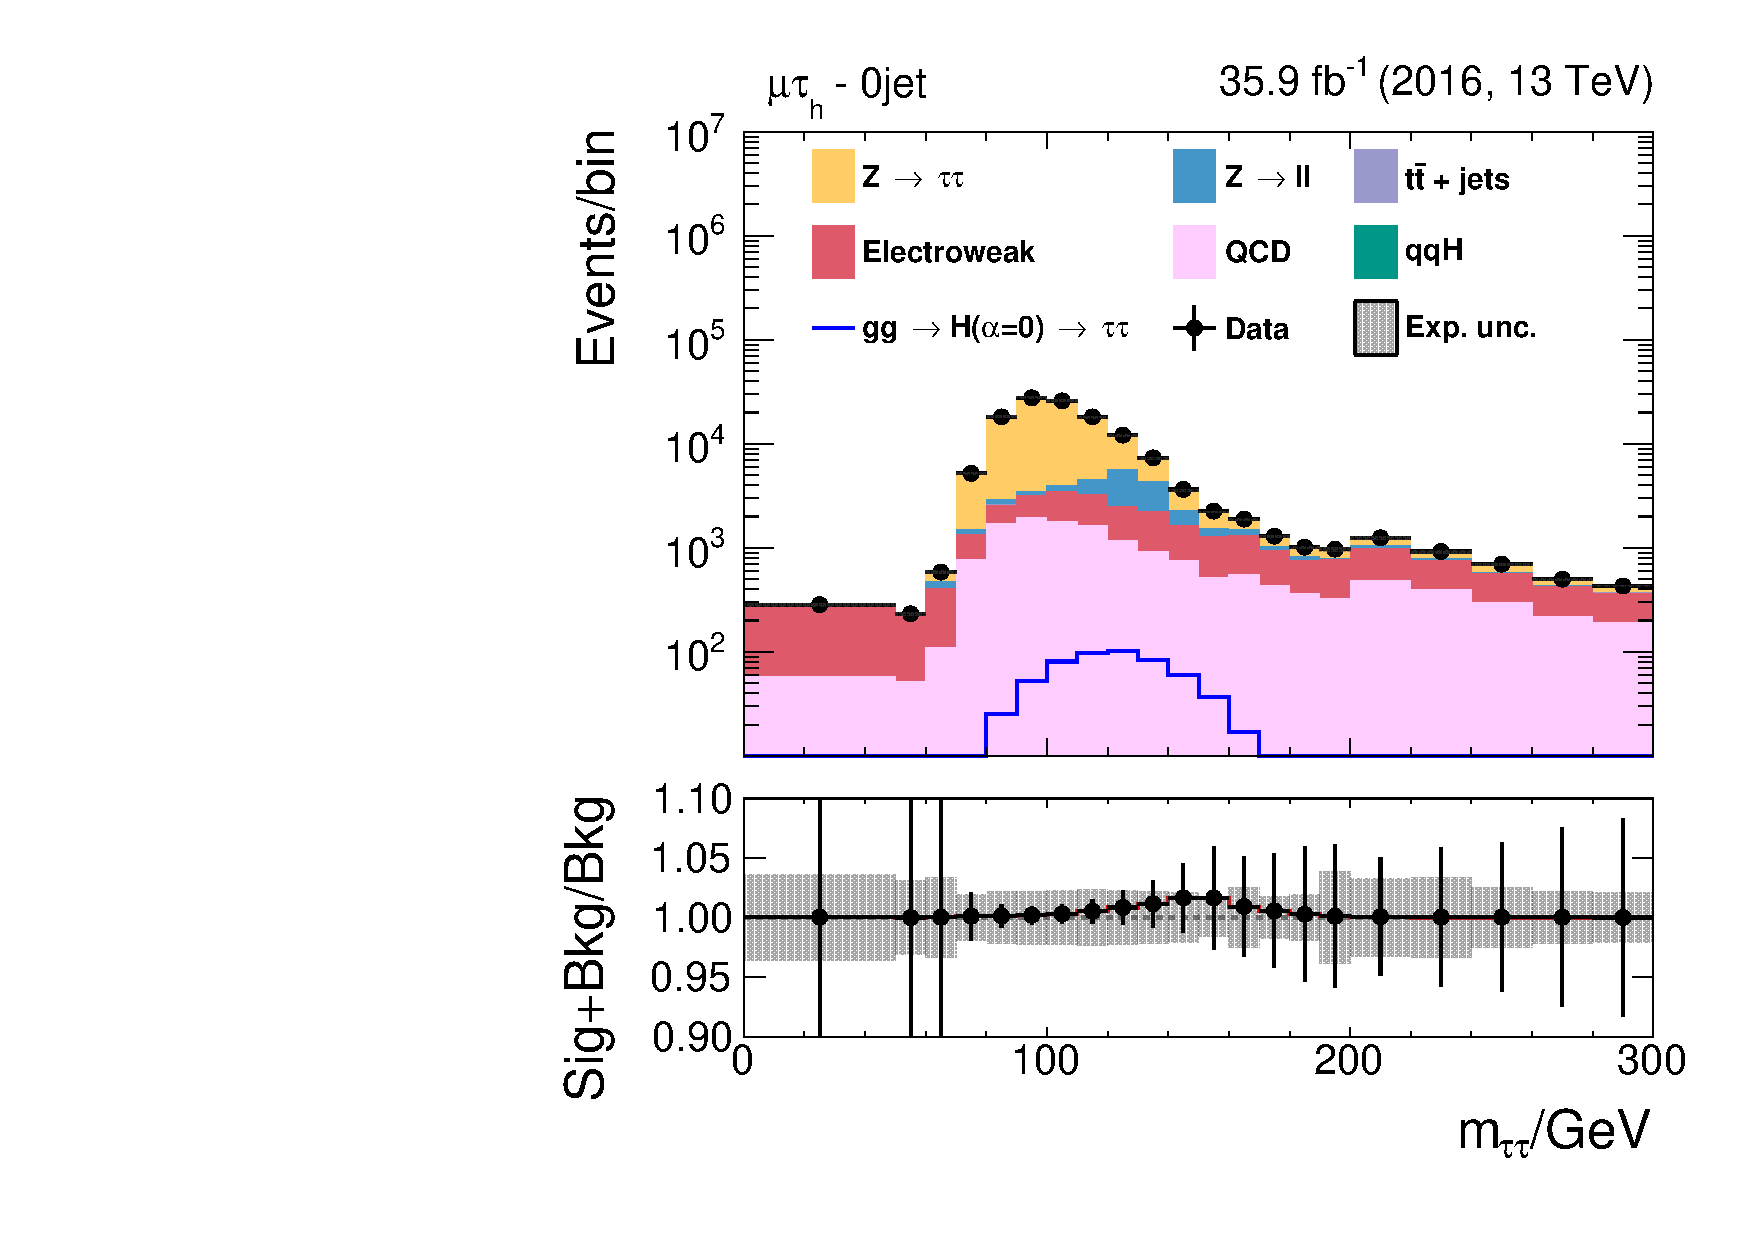
\includegraphics[width=.5\textwidth]{Figures/statana/Postfit_JEC_mela3D/postfit_fit_s_htt_mt_1_13TeV.pdf}\\
        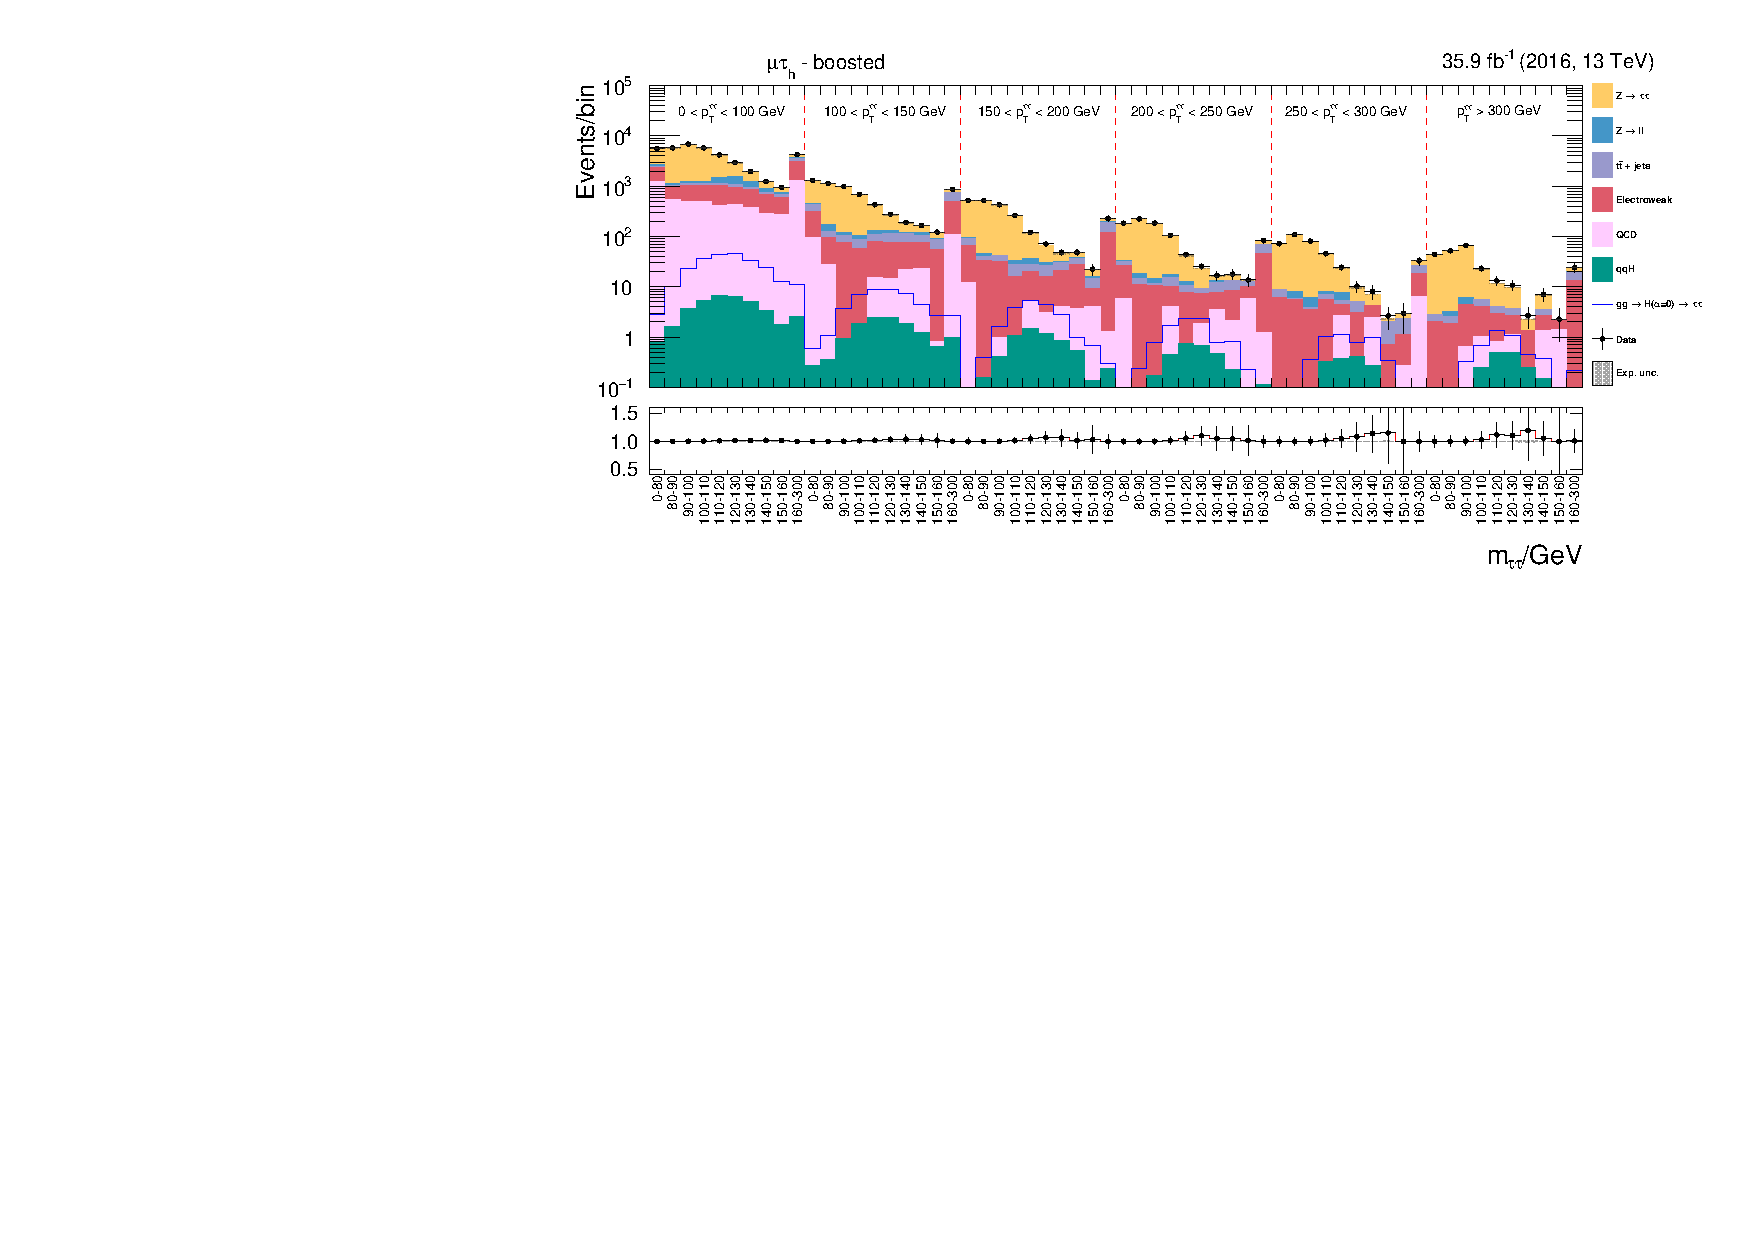
\includegraphics[width=\textwidth]{Figures/statana/Postfit_JEC_mela3D/postfit_fit_s_htt_mt_2_13TeV.pdf}    
    \caption{Postfit distributions of the \textit{0-jet} and \textit{boosted} categories in the \mutau{} channel  using the MELA approach.}
\end{figure}
\begin{figure}[h!]
    \centering
        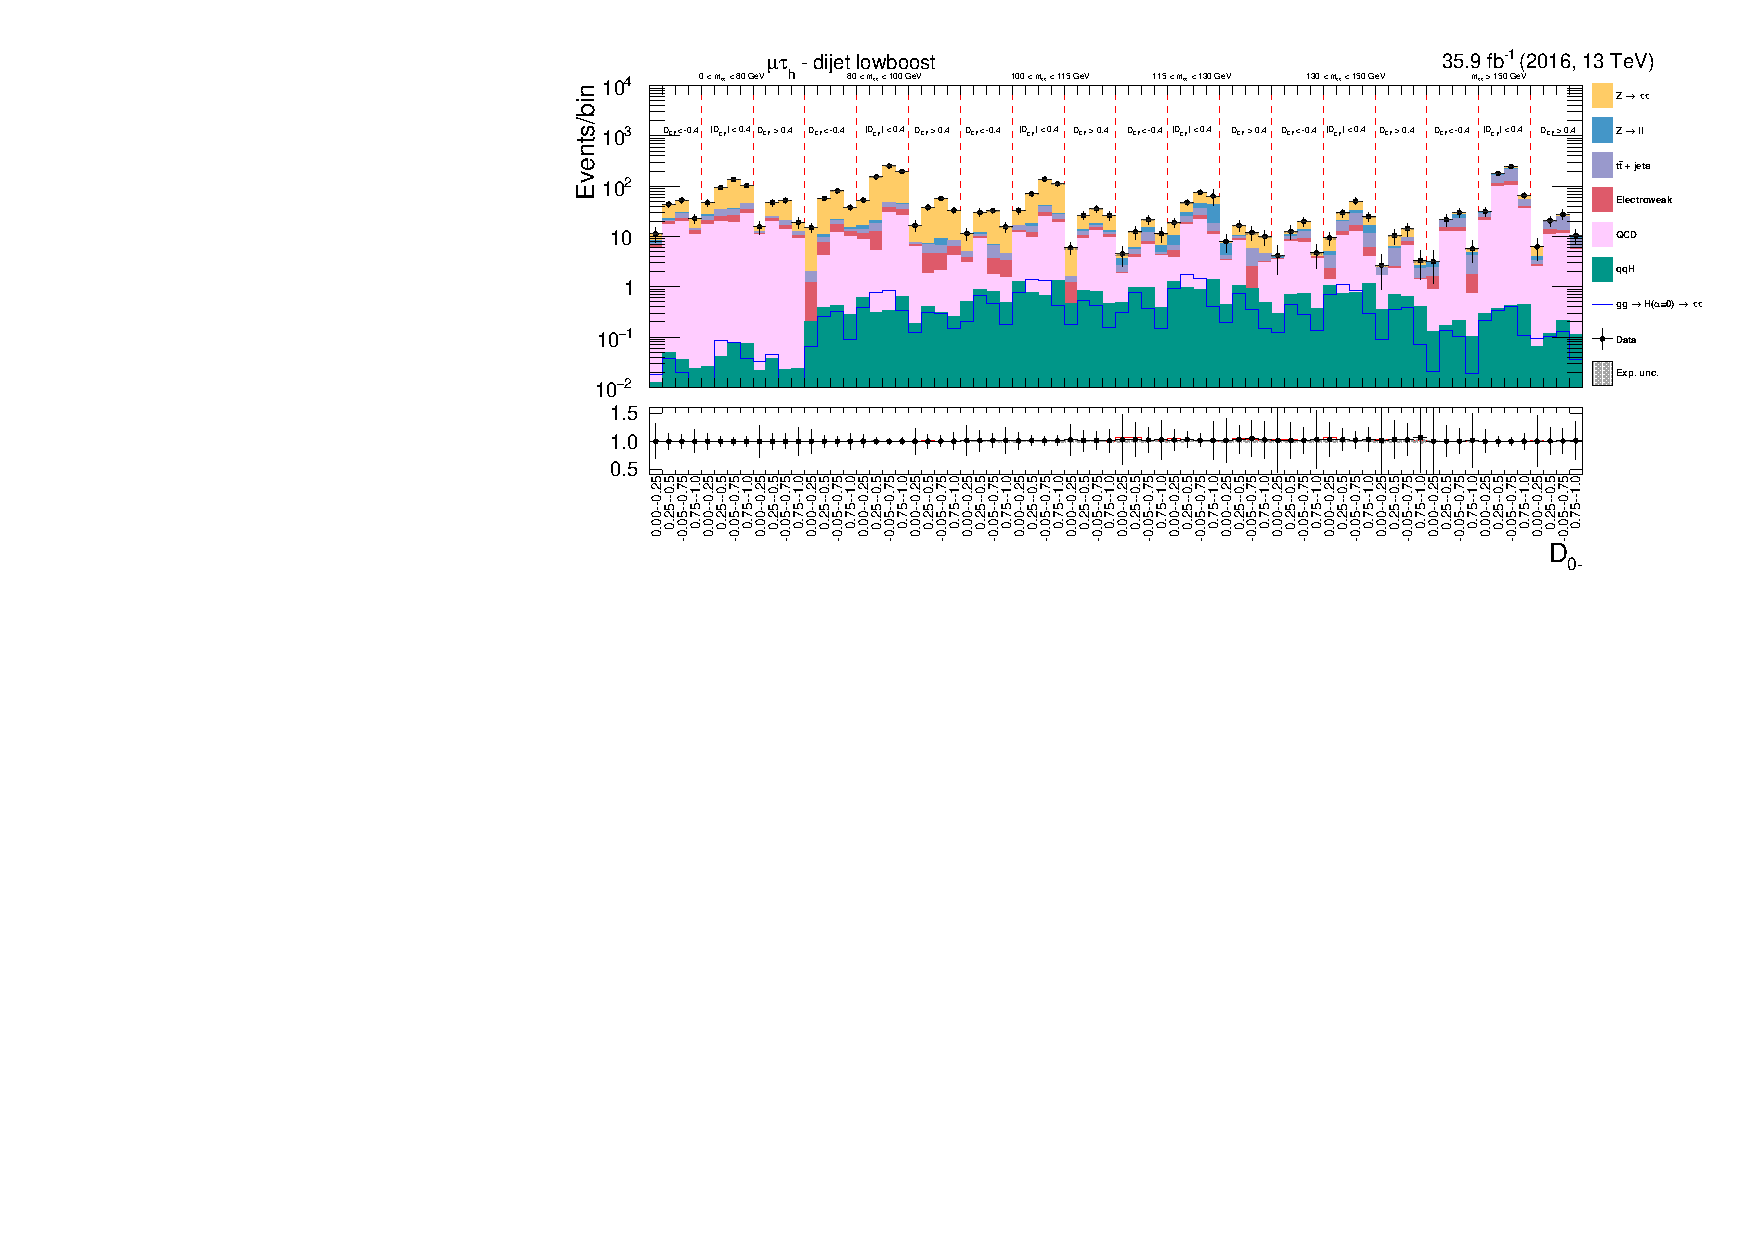
\includegraphics[width=\textwidth]{Figures/statana/Postfit_JEC_mela3D/postfit_fit_s_htt_mt_3_13TeV.pdf}\\
        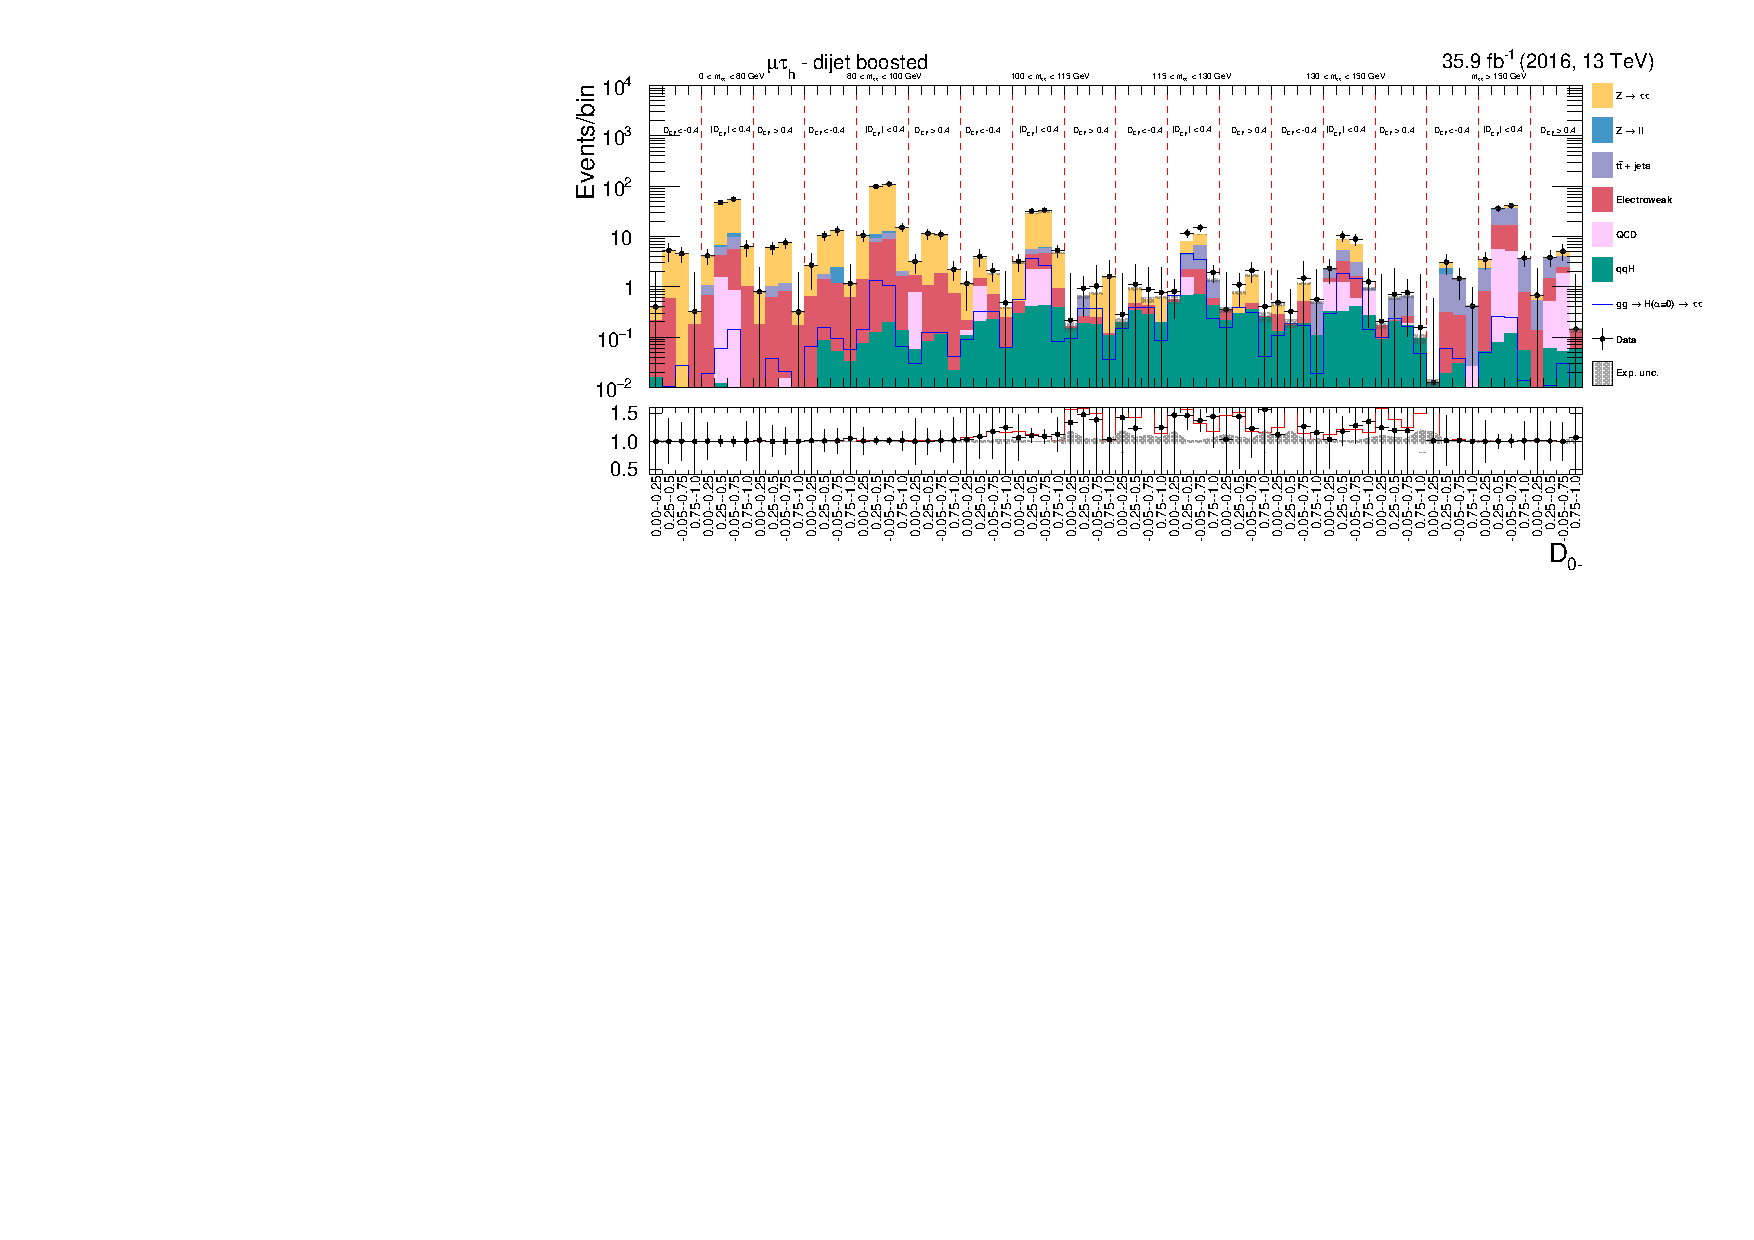
\includegraphics[width=\textwidth]{Figures/statana/Postfit_JEC_mela3D/postfit_fit_s_htt_mt_4_13TeV.pdf}
    \caption{Postfit distributions of the \textit{dijet lowboost} and \textit{dijet boosted} categories in the \mutau{} channel  using the MELA approach.}
\end{figure}
\clearpage
\begin{figure}[h!]
    \centering
        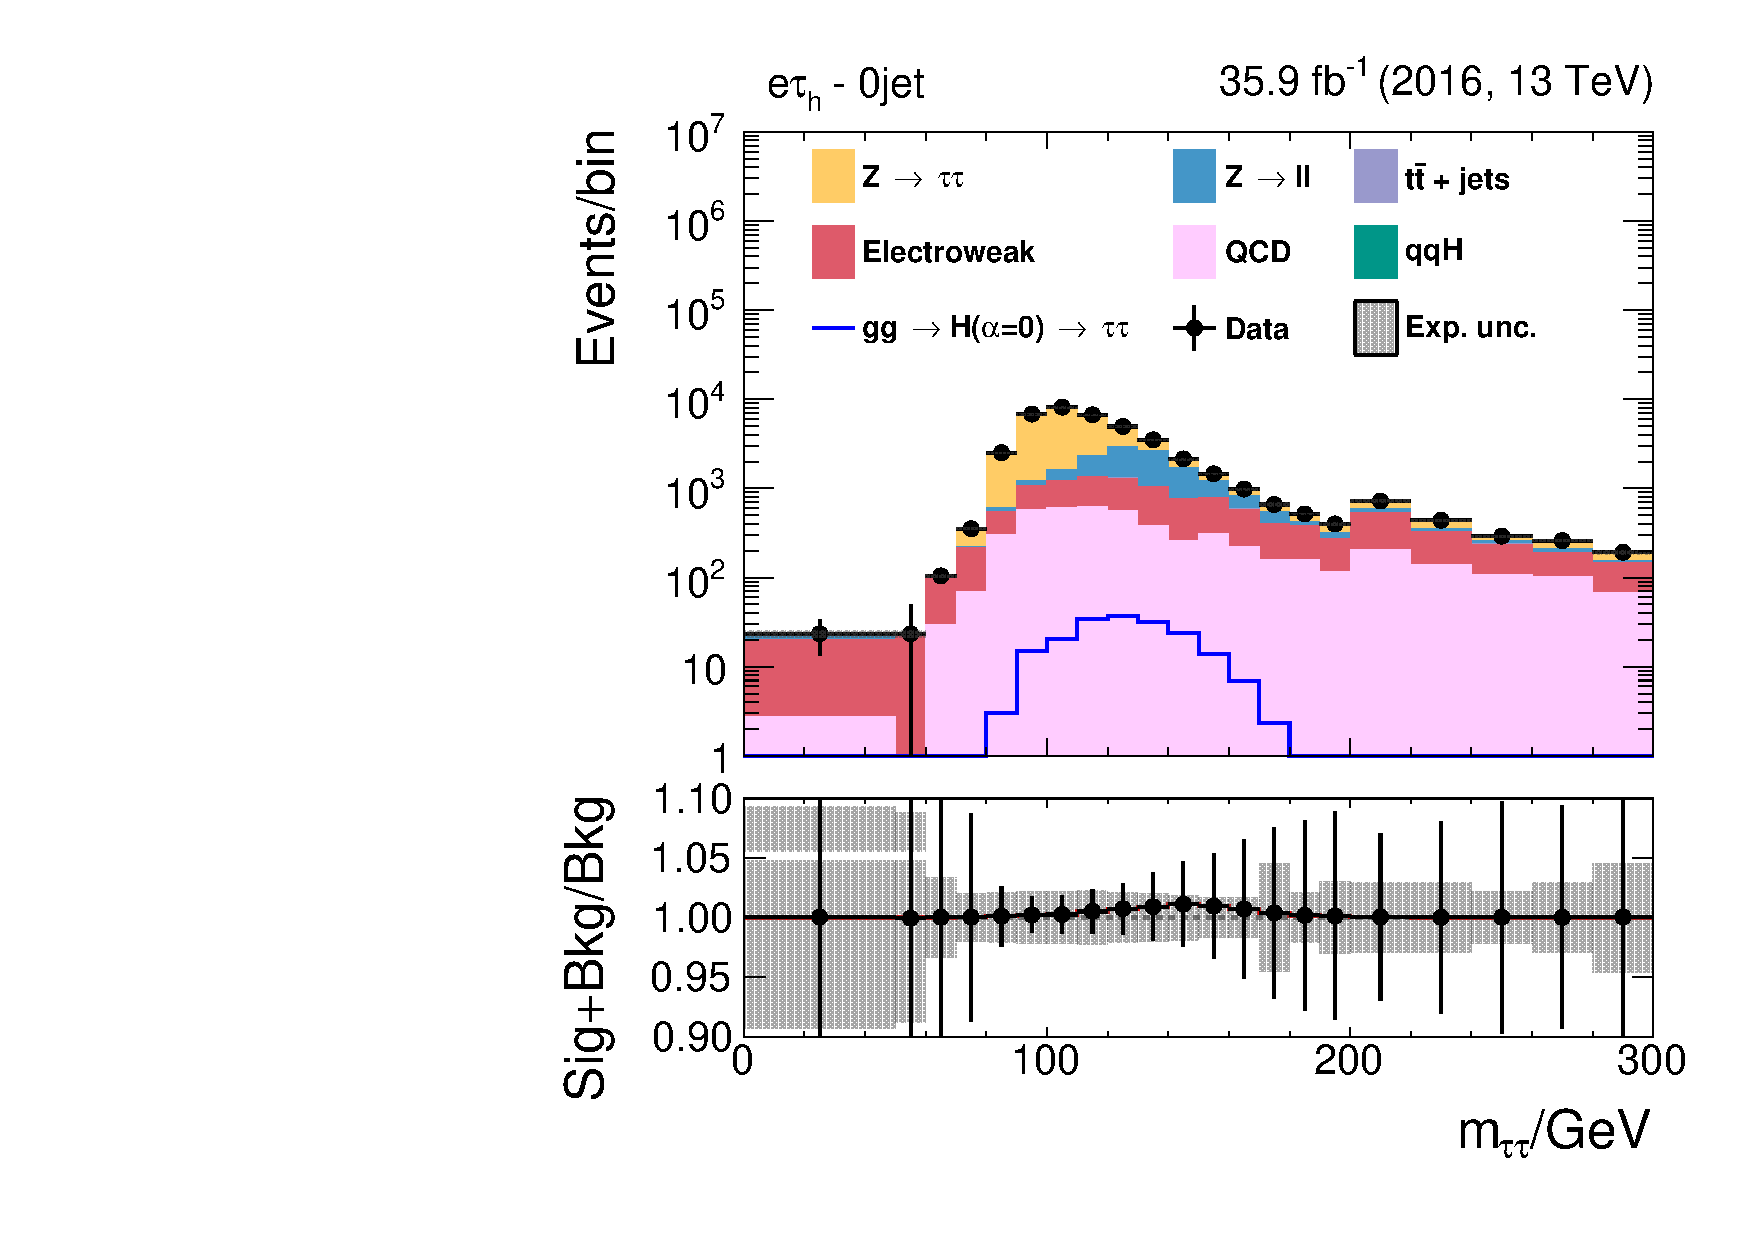
\includegraphics[width=.5\textwidth]{Figures/statana/Postfit_JEC_mela3D/postfit_fit_s_htt_et_1_13TeV.pdf}\\
        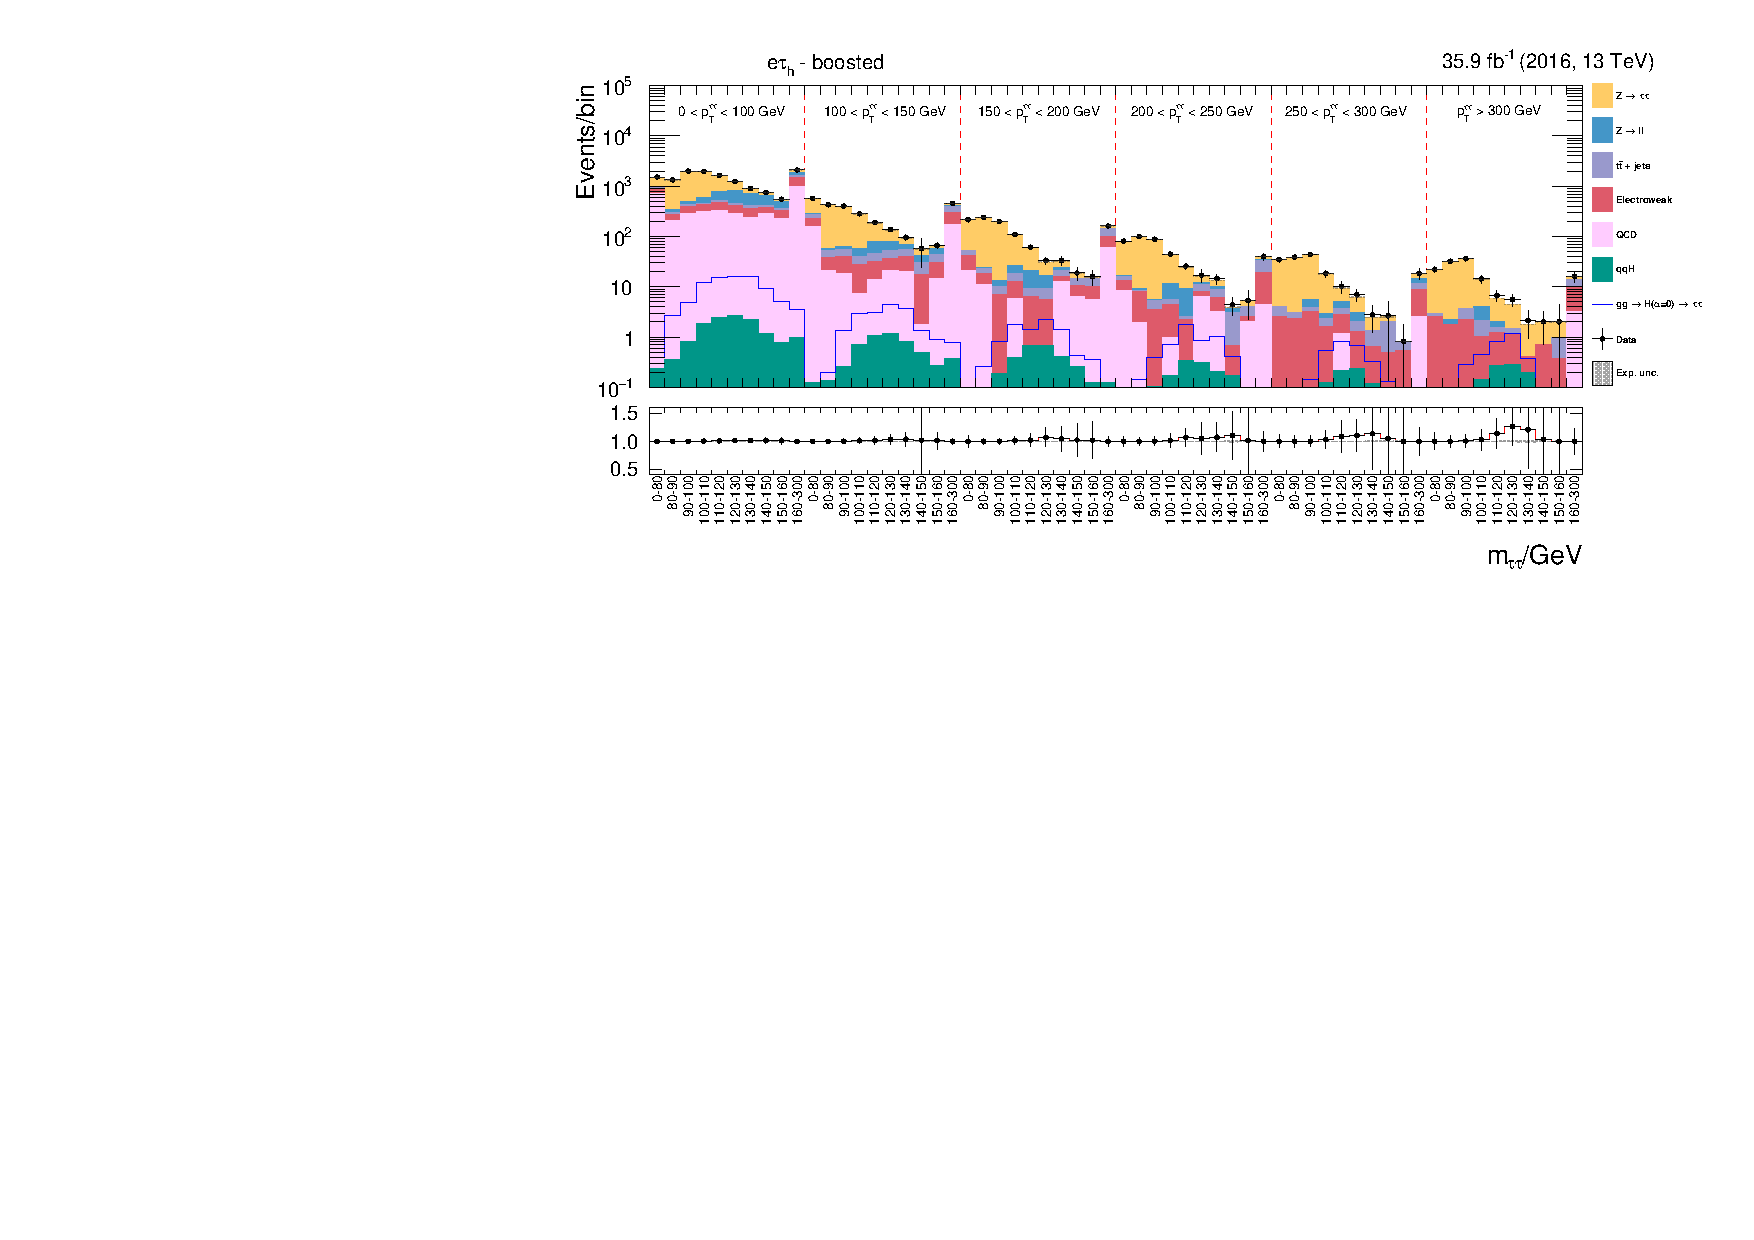
\includegraphics[width=\textwidth]{Figures/statana/Postfit_JEC_mela3D/postfit_fit_s_htt_et_2_13TeV.pdf}
    \caption{Postfit distributions of the \textit{0-jet} and \textit{boosted} categories in the \etau{} channel  using the MELA approach.}
\end{figure} 
\begin{figure}[h!]
    \centering       
        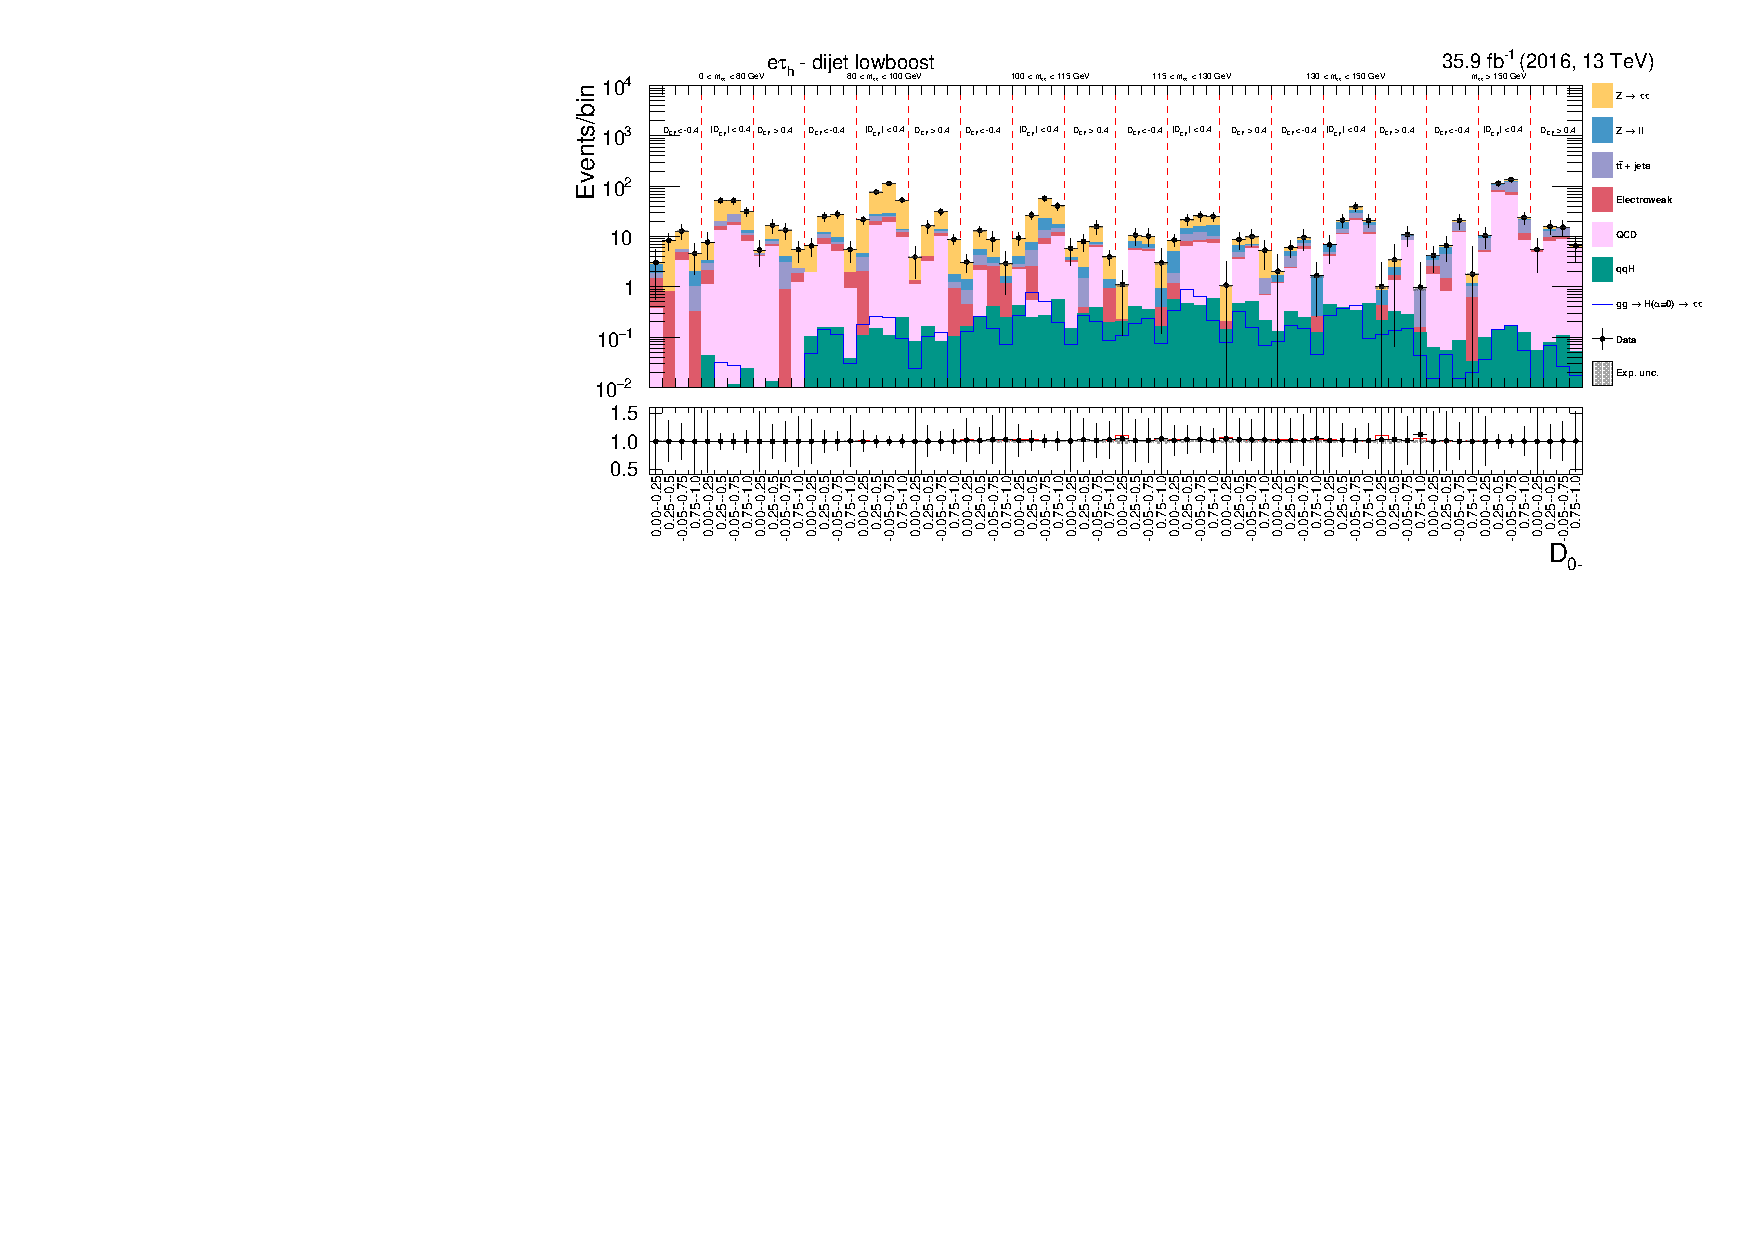
\includegraphics[width=\textwidth]{Figures/statana/Postfit_JEC_mela3D/postfit_fit_s_htt_et_3_13TeV.pdf}\\
        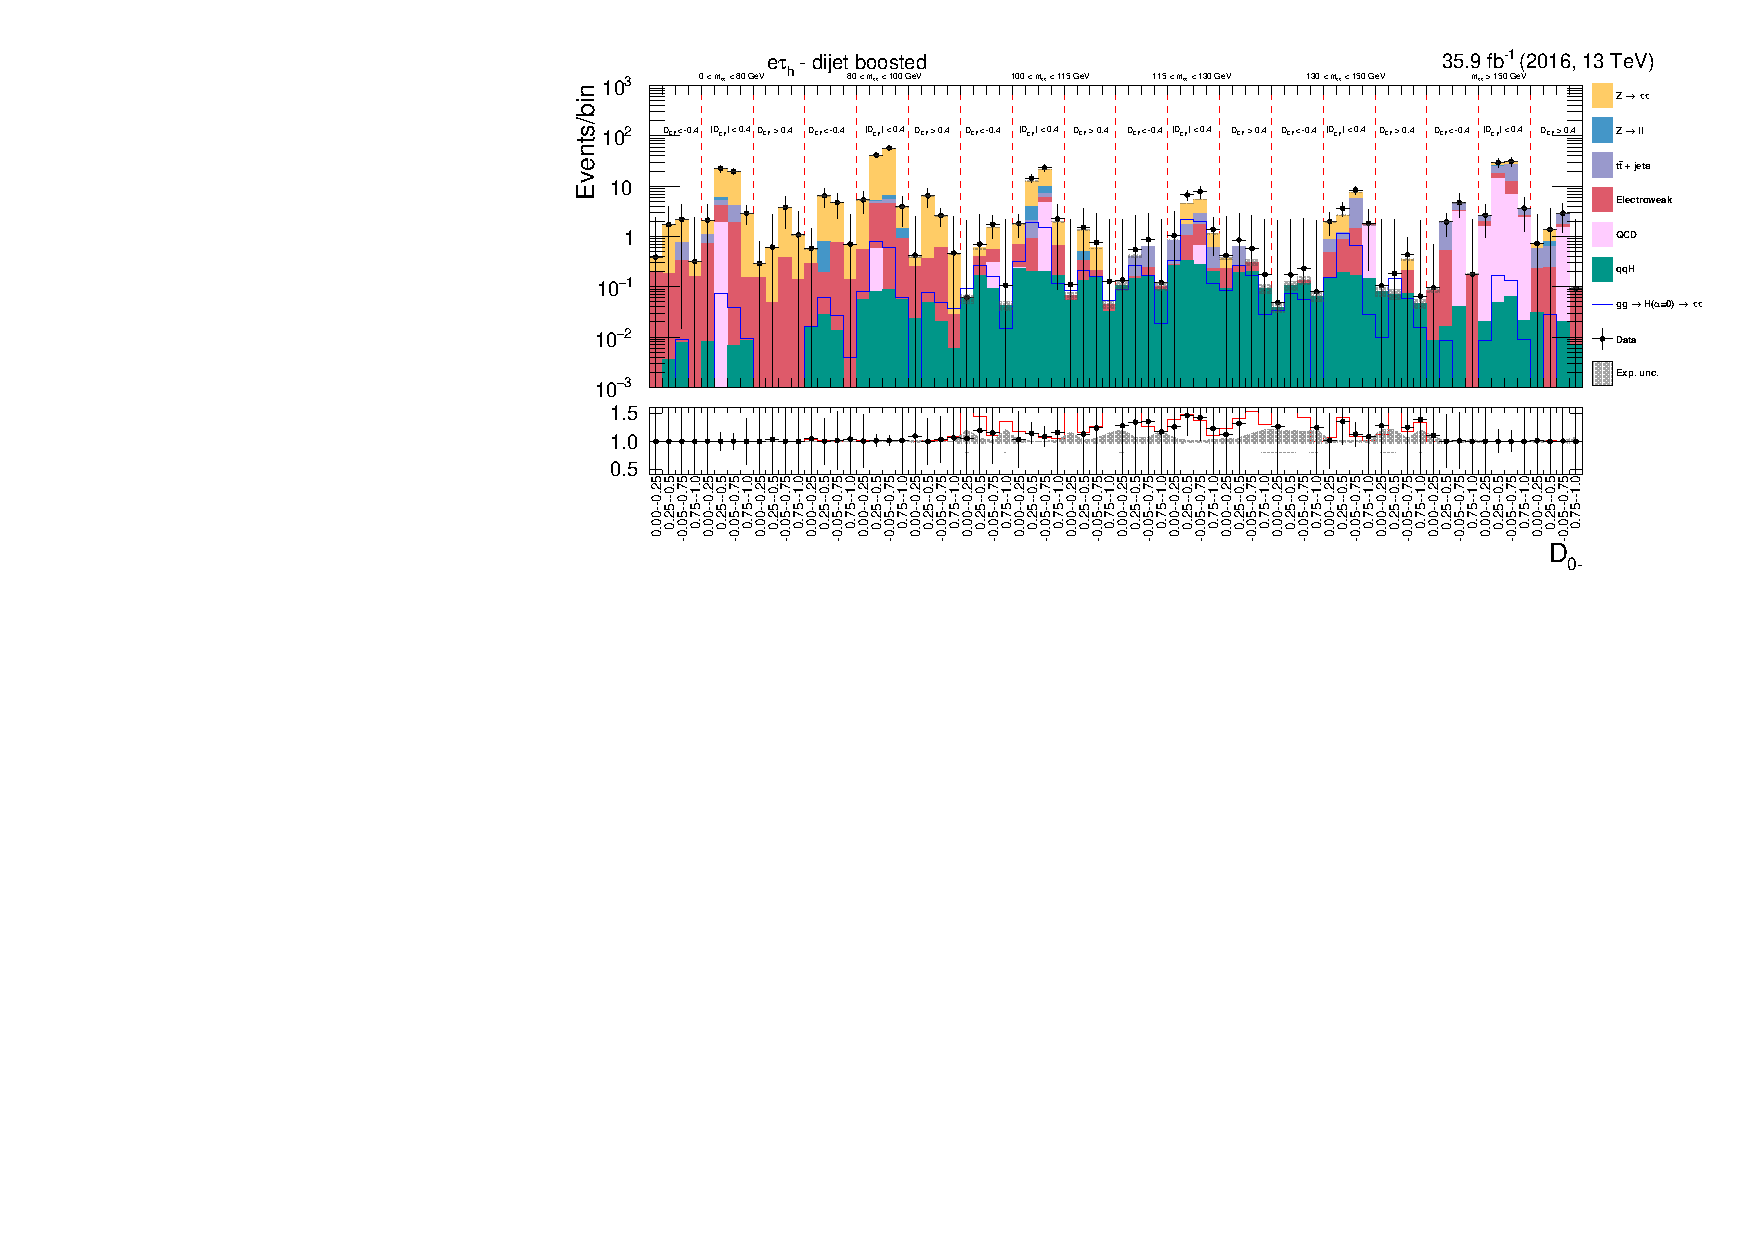
\includegraphics[width=\textwidth]{Figures/statana/Postfit_JEC_mela3D/postfit_fit_s_htt_et_4_13TeV.pdf}
    \caption{Postfit distributions of the \textit{dijet lowboost} and \textit{dijet boosted} categories in the \etau{} channel  using the MELA approach.}
\end{figure}
\clearpage
\begin{figure}[h!]
    \centering
        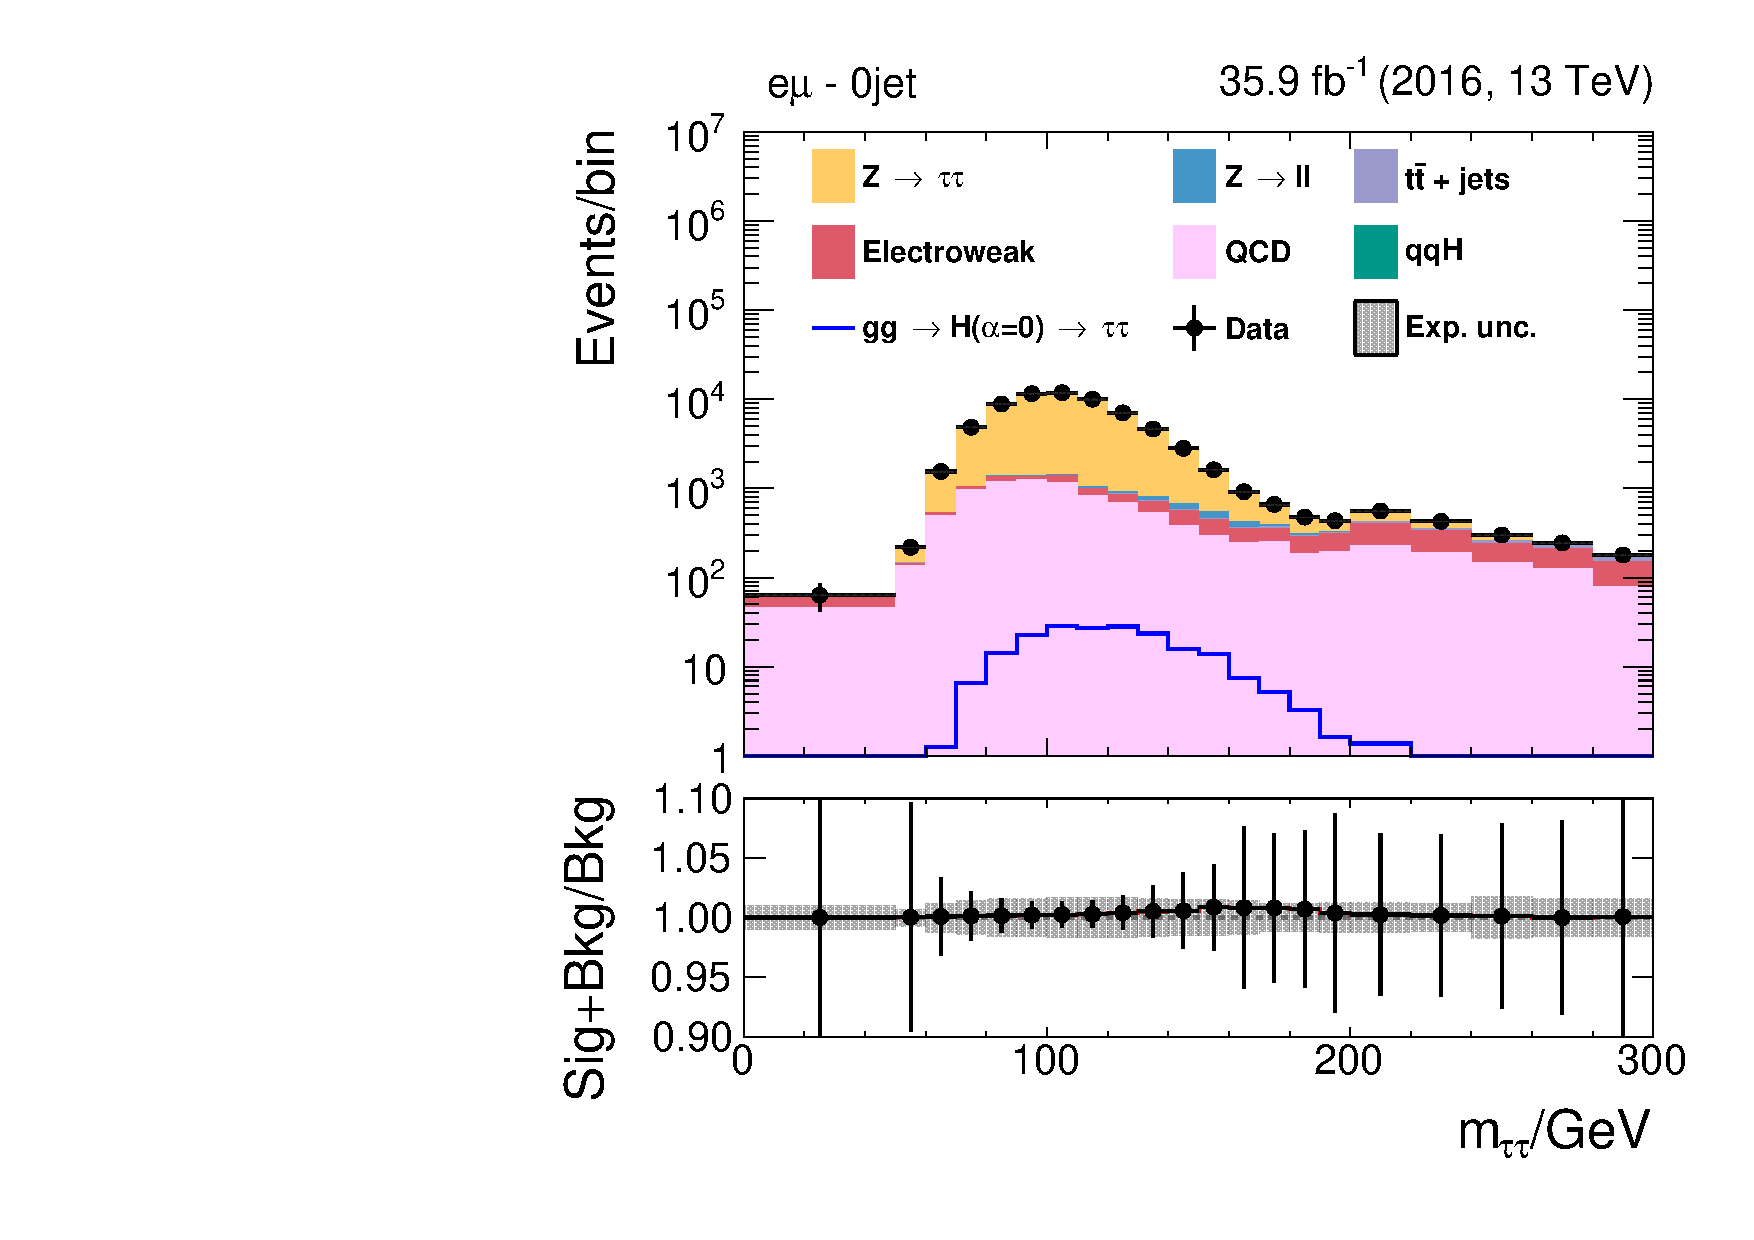
\includegraphics[width=0.5\textwidth]{Figures/statana/Postfit_JEC_mela3D/postfit_fit_s_htt_em_1_13TeV.pdf}\\
        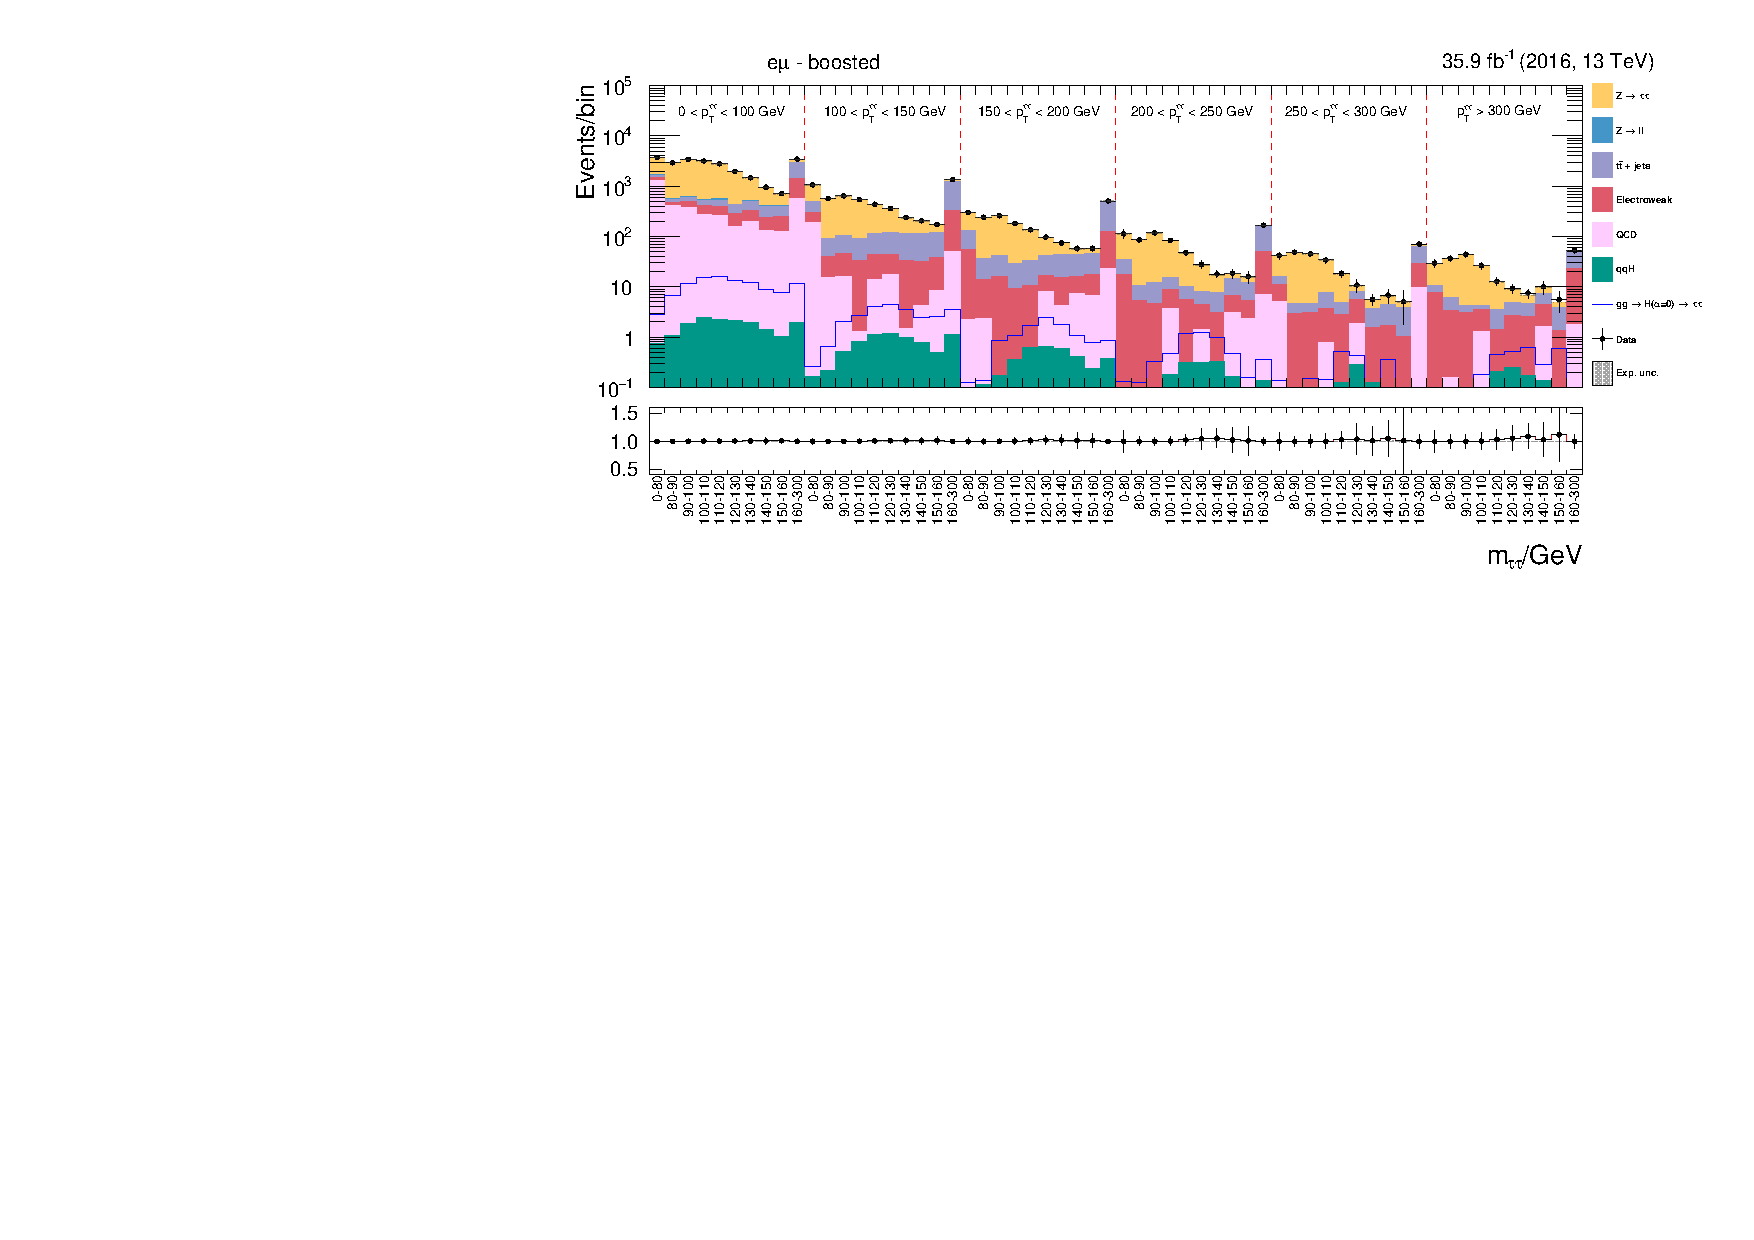
\includegraphics[width=\textwidth]{Figures/statana/Postfit_JEC_mela3D/postfit_fit_s_htt_em_2_13TeV.pdf}
    \caption{Postfit distributions of the \textit{0-jet} and \textit{boosted} categories in the \emu{} channel  using the MELA approach.}
\end{figure}
\begin{figure}[h!]
    \centering
        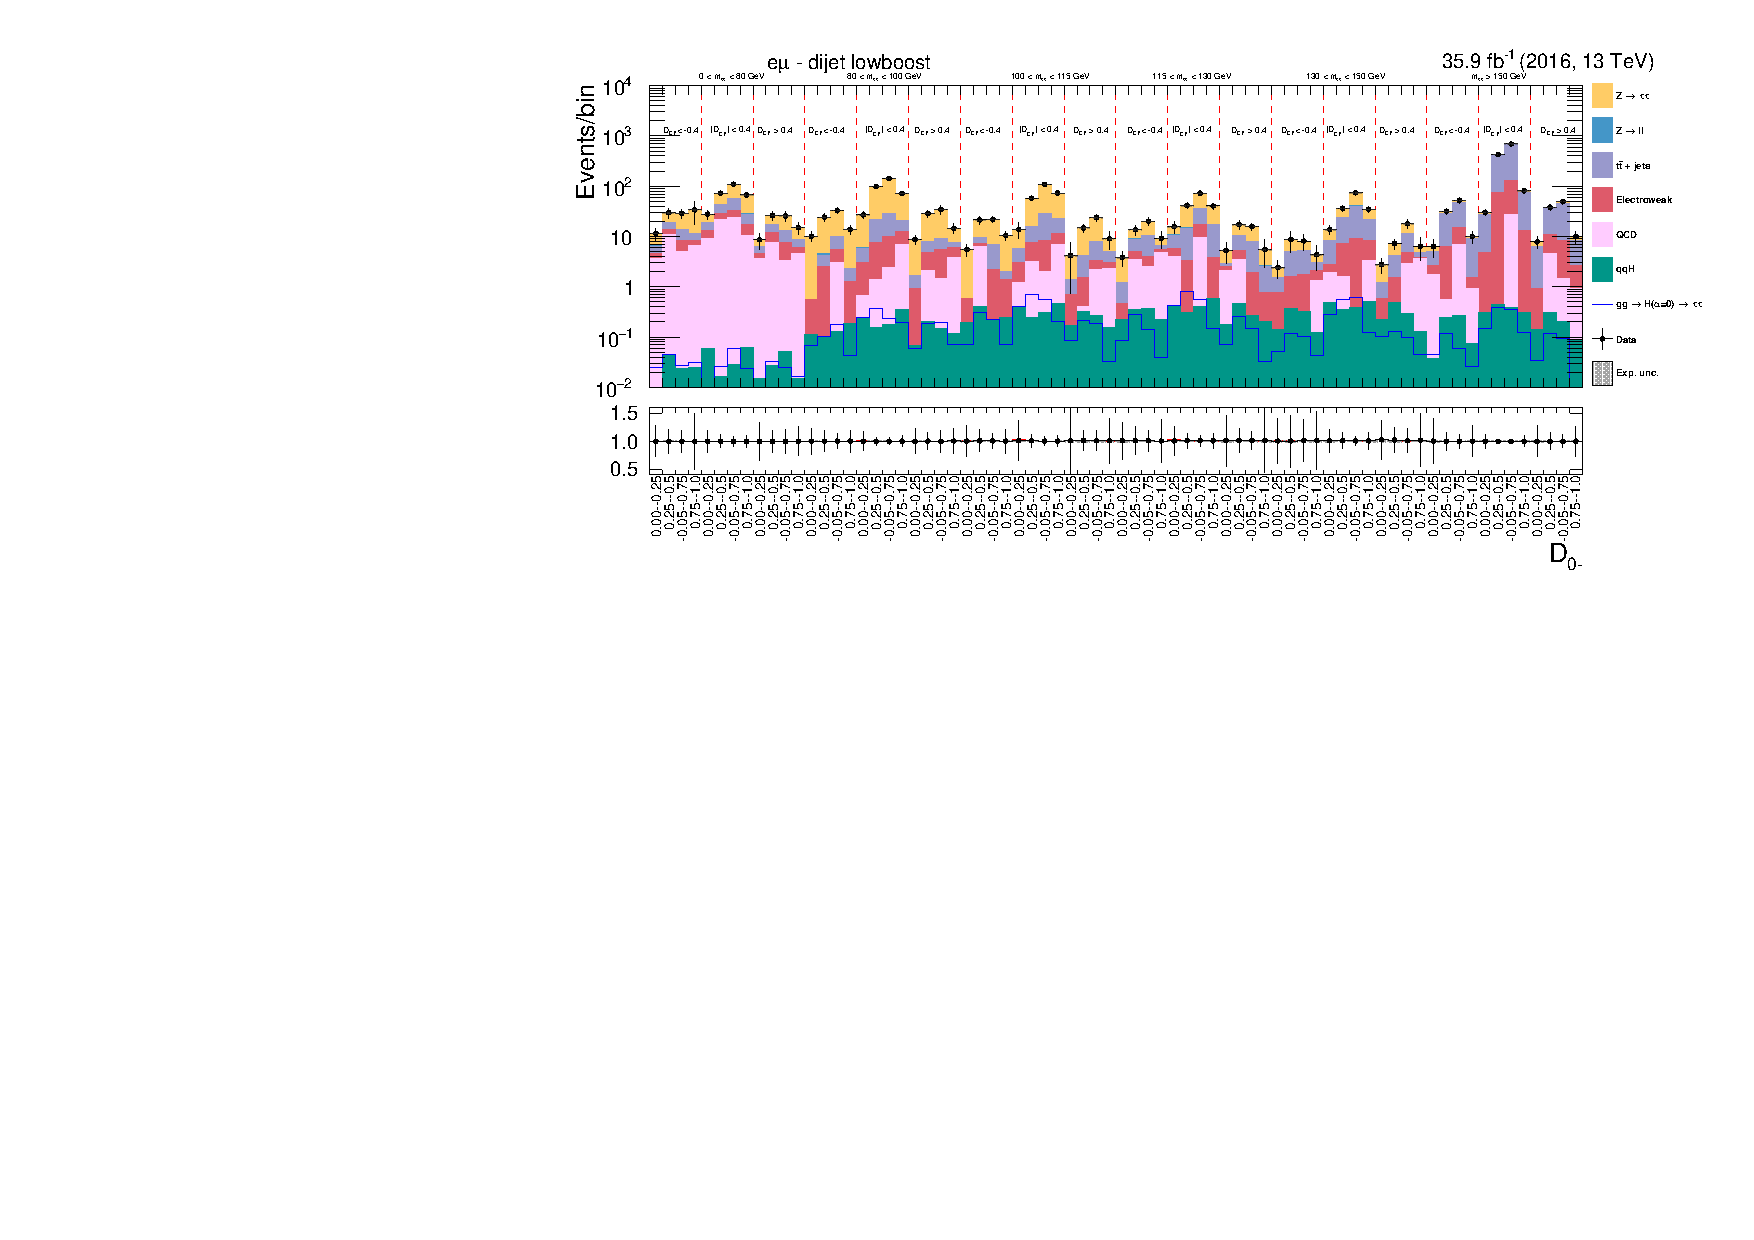
\includegraphics[width=\textwidth]{Figures/statana/Postfit_JEC_mela3D/postfit_fit_s_htt_em_3_13TeV.pdf}\\
        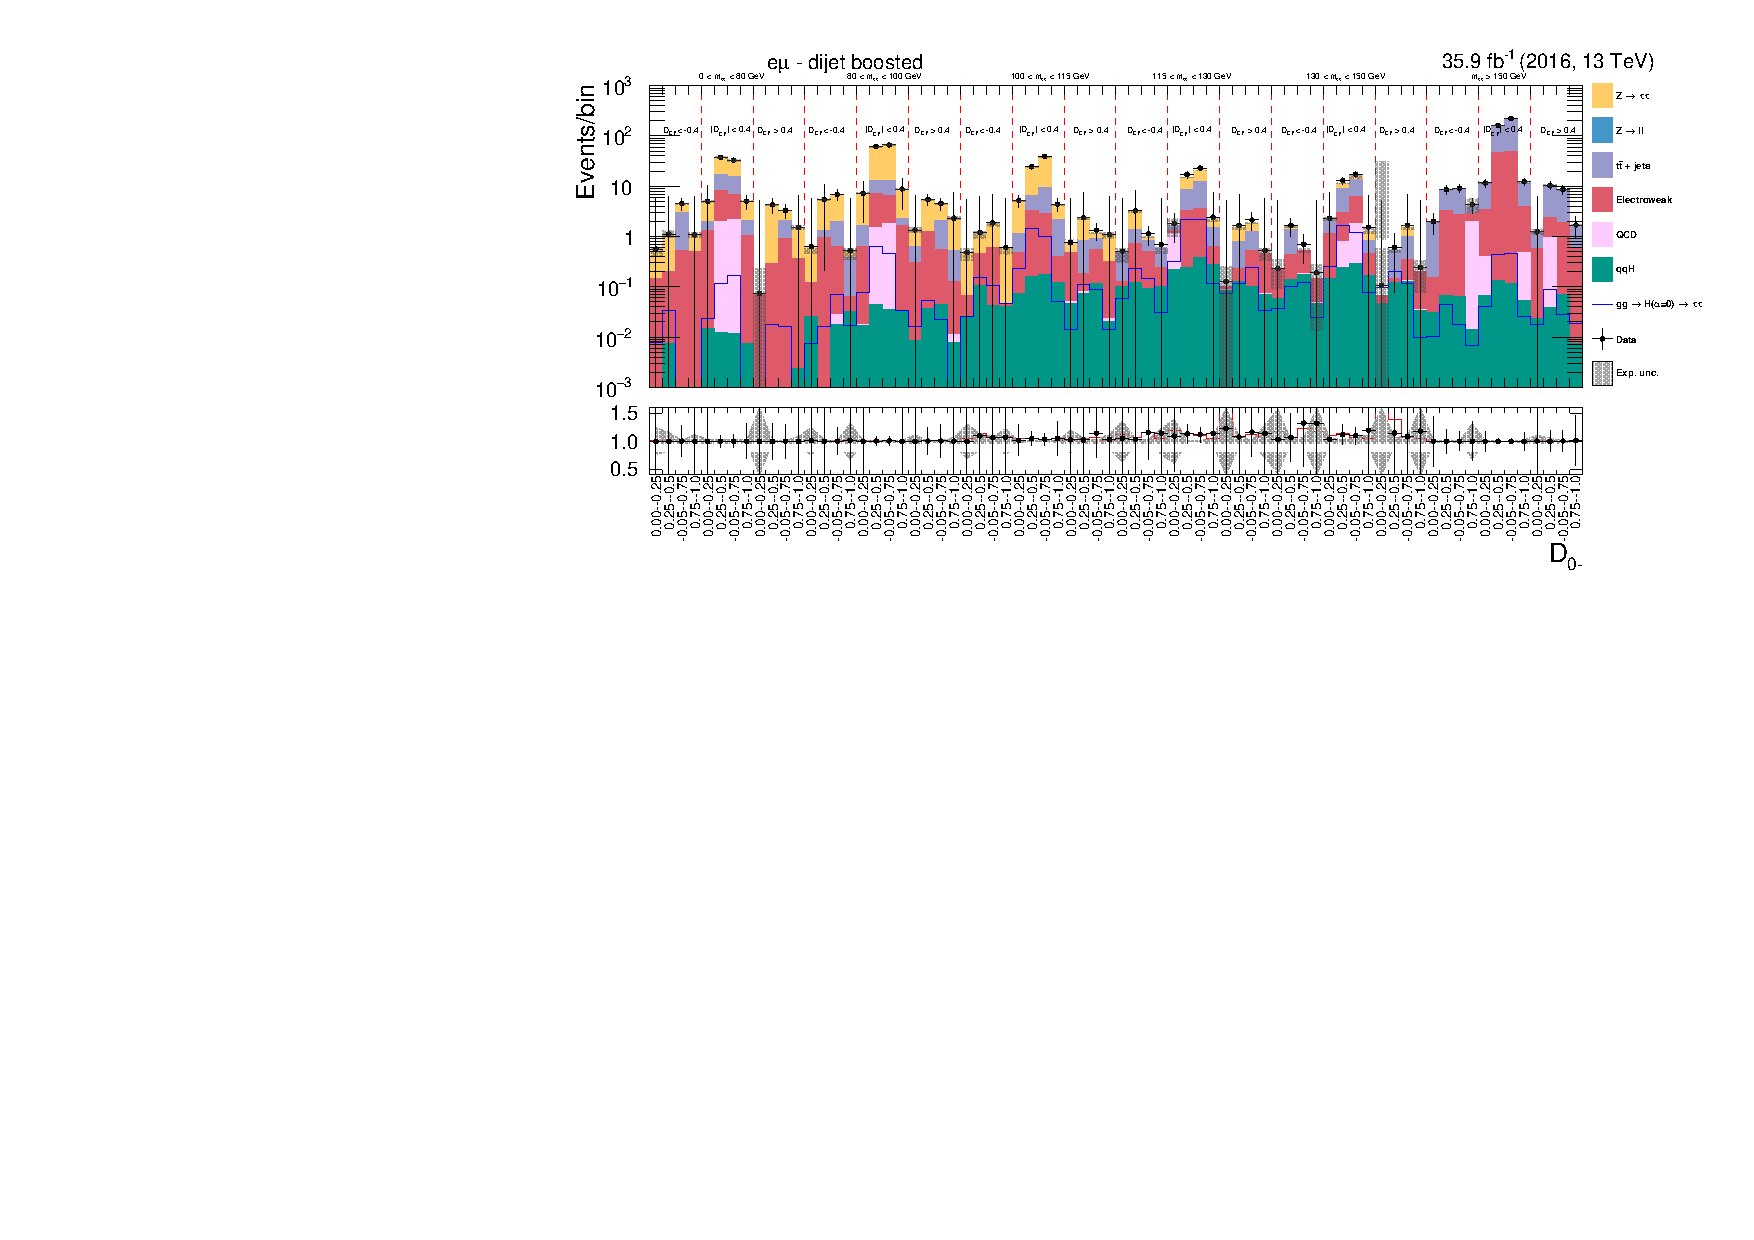
\includegraphics[width=\textwidth]{Figures/statana/Postfit_JEC_mela3D/postfit_fit_s_htt_em_4_13TeV.pdf}
    \caption{Postfit distributions of the \textit{dijet lowboost} and \textit{dijet boosted} categories in the \emu{} channel  using the MELA approach.}\label{SUPPLE:SA:postfit_em_2jet}
\end{figure}
\clearpage

\subsection{Prefit distributions for \jdphi}

\begin{figure}[h!]
    \centering
        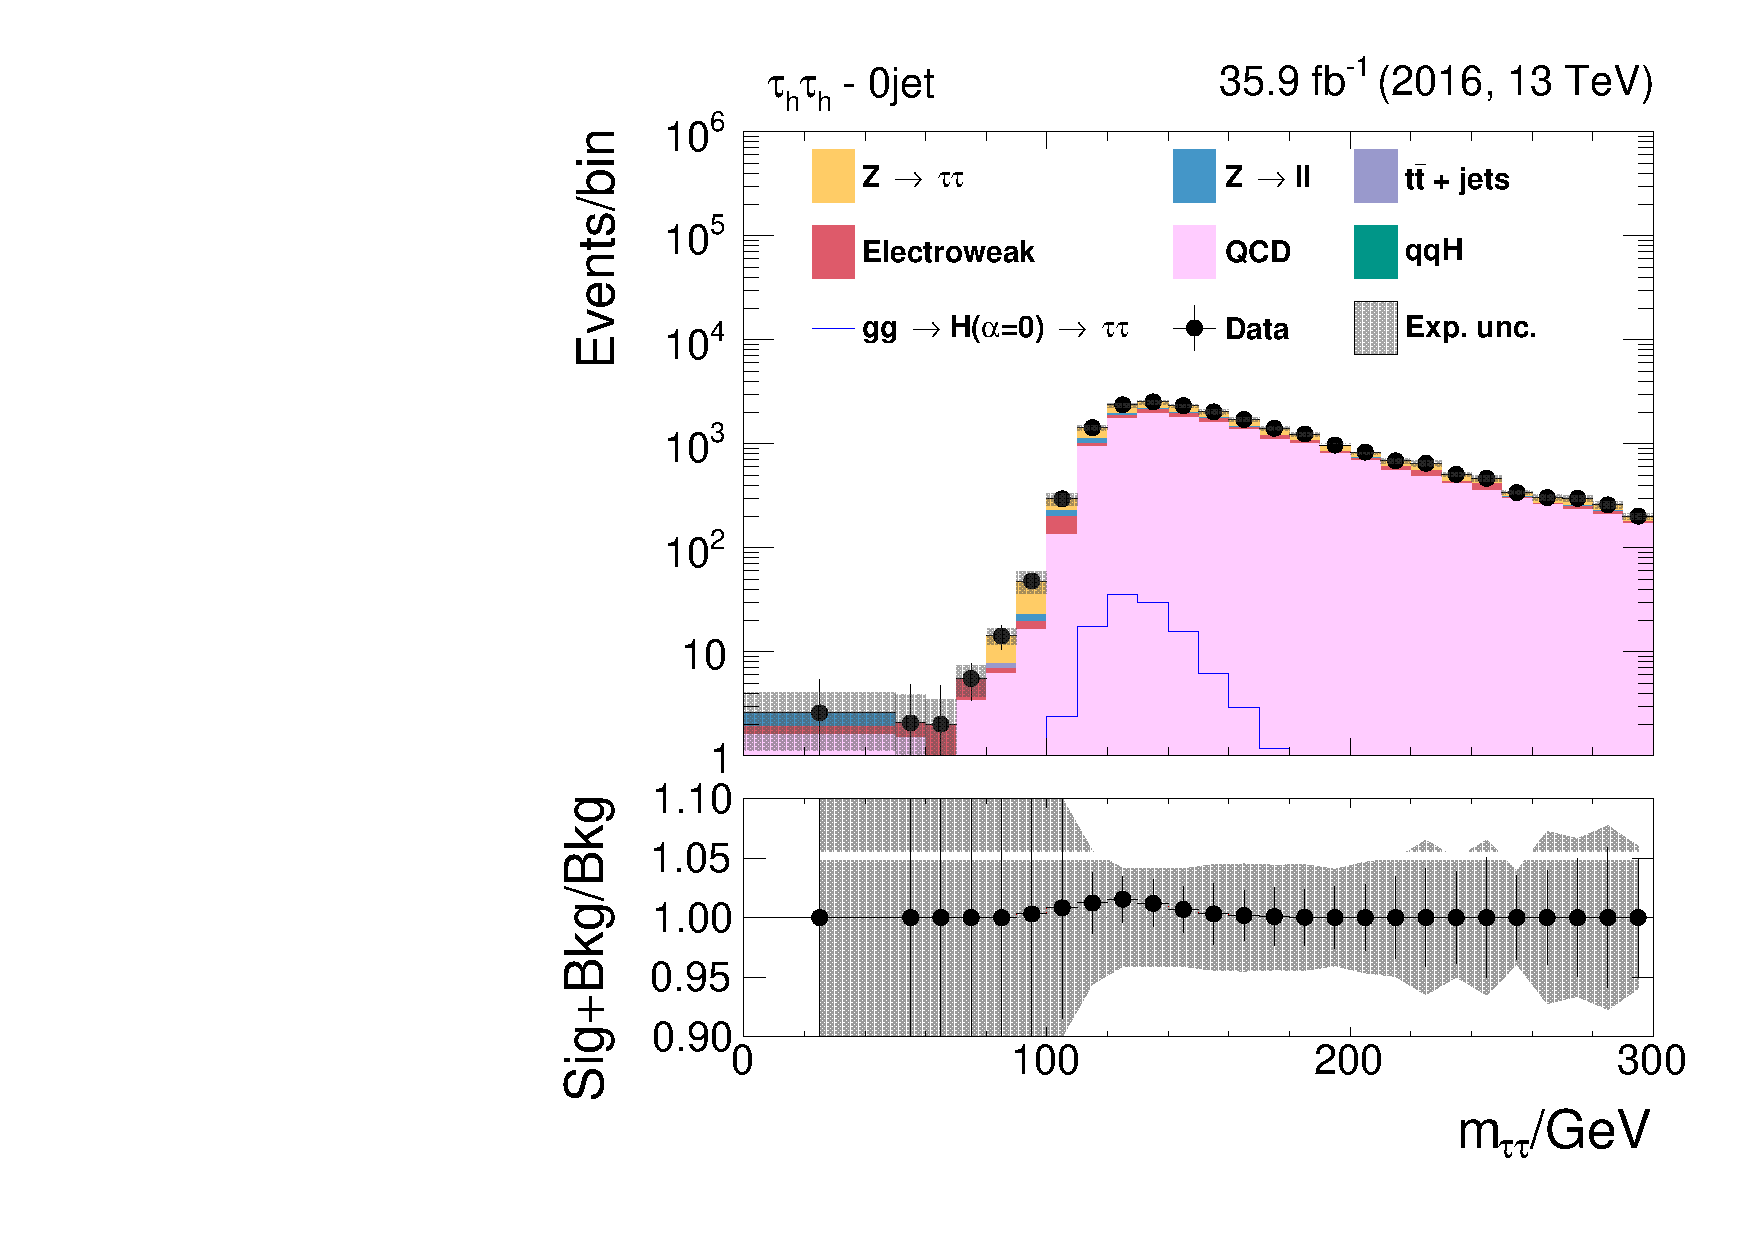
\includegraphics[width=.5\textwidth]{Figures/statana/Postfit_JEC_jdphi/prefit_htt_tt_1_13TeV.pdf}\\
        \includegraphics[width=\textwidth]{Figures/statana/Postfit_JEC_jdphi/prefit_htt_tt_2_13TeV.pdf}
        \caption{Prefit distributions of the \textit{0-jet} and \textit{boosted} categories in the \tautau{} channel  using \jdphi{}.}
\end{figure}
\begin{figure}[h!]
        \centering
        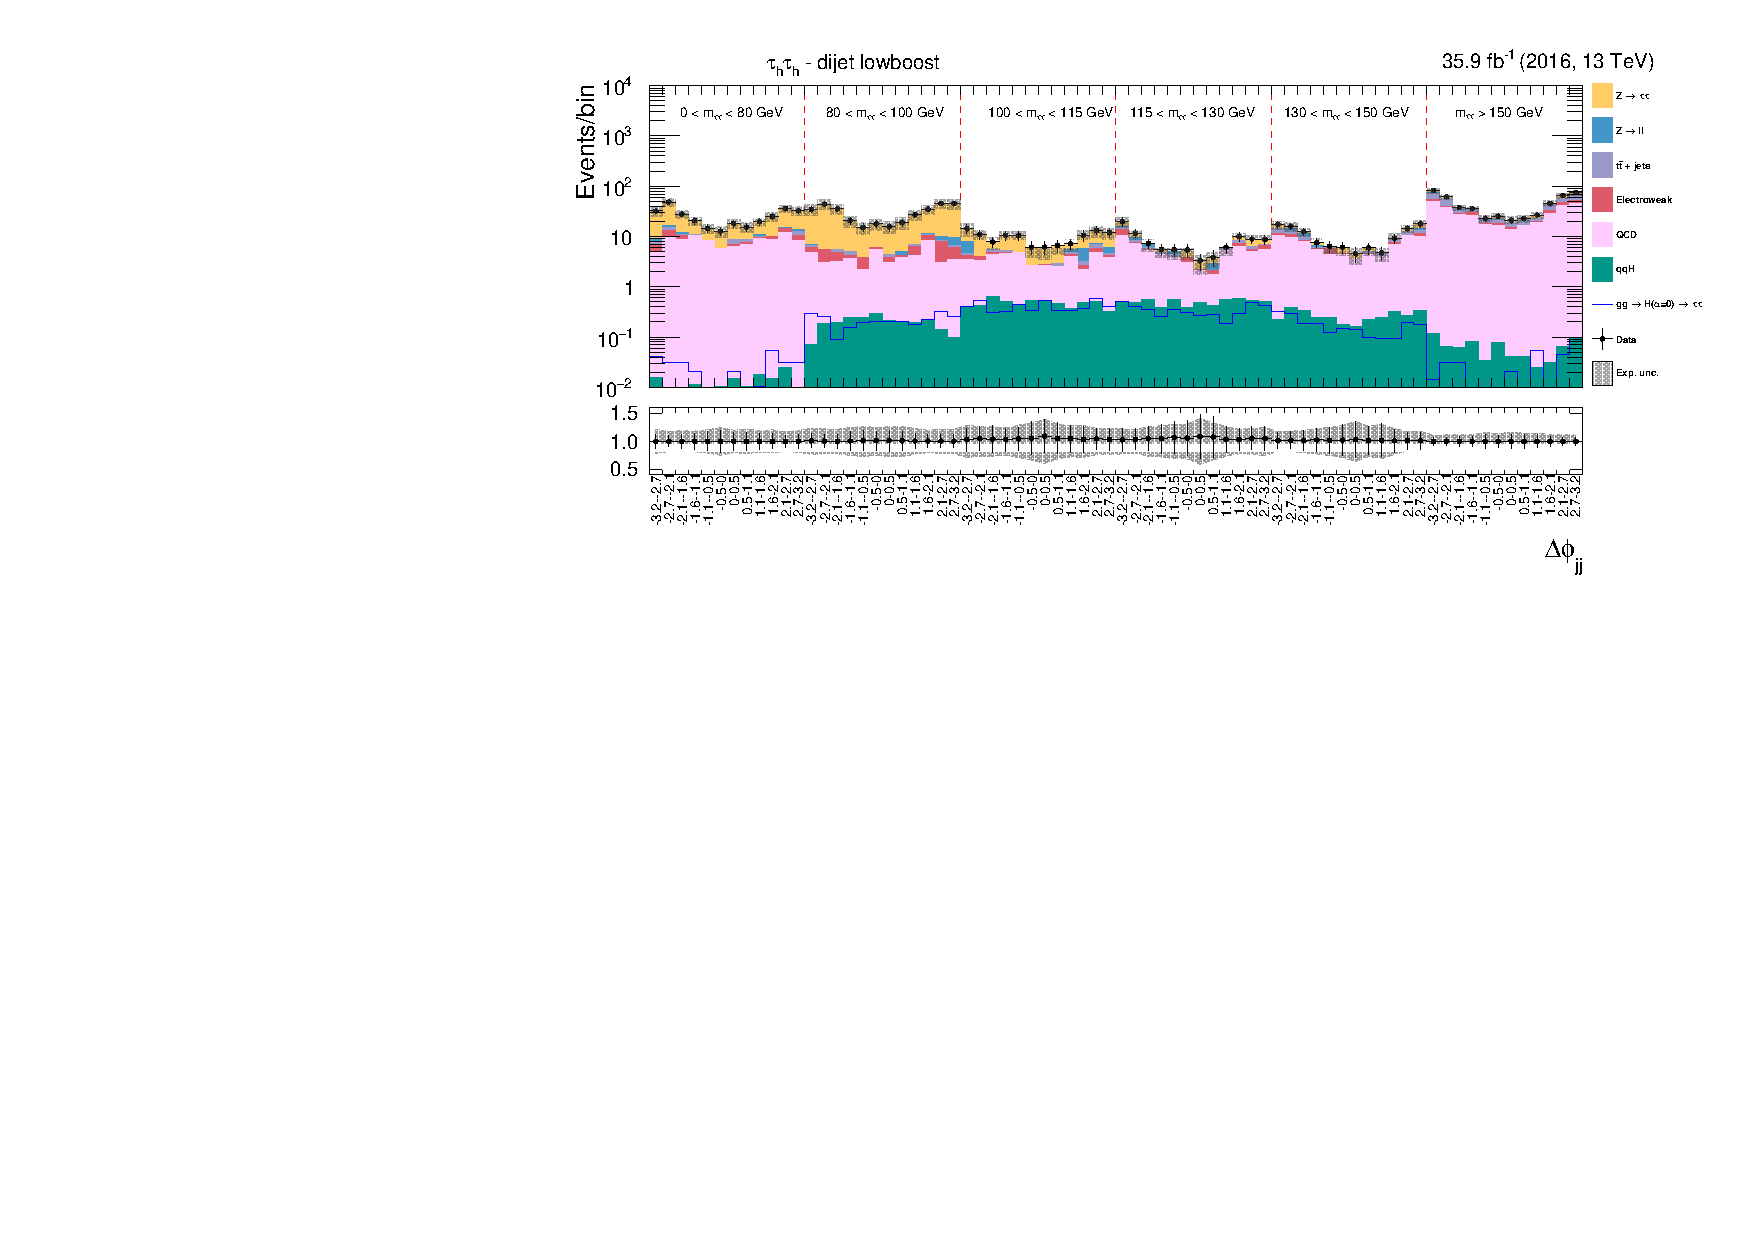
\includegraphics[width=\textwidth]{Figures/statana/Postfit_JEC_jdphi/prefit_htt_tt_3_13TeV.pdf}\\
        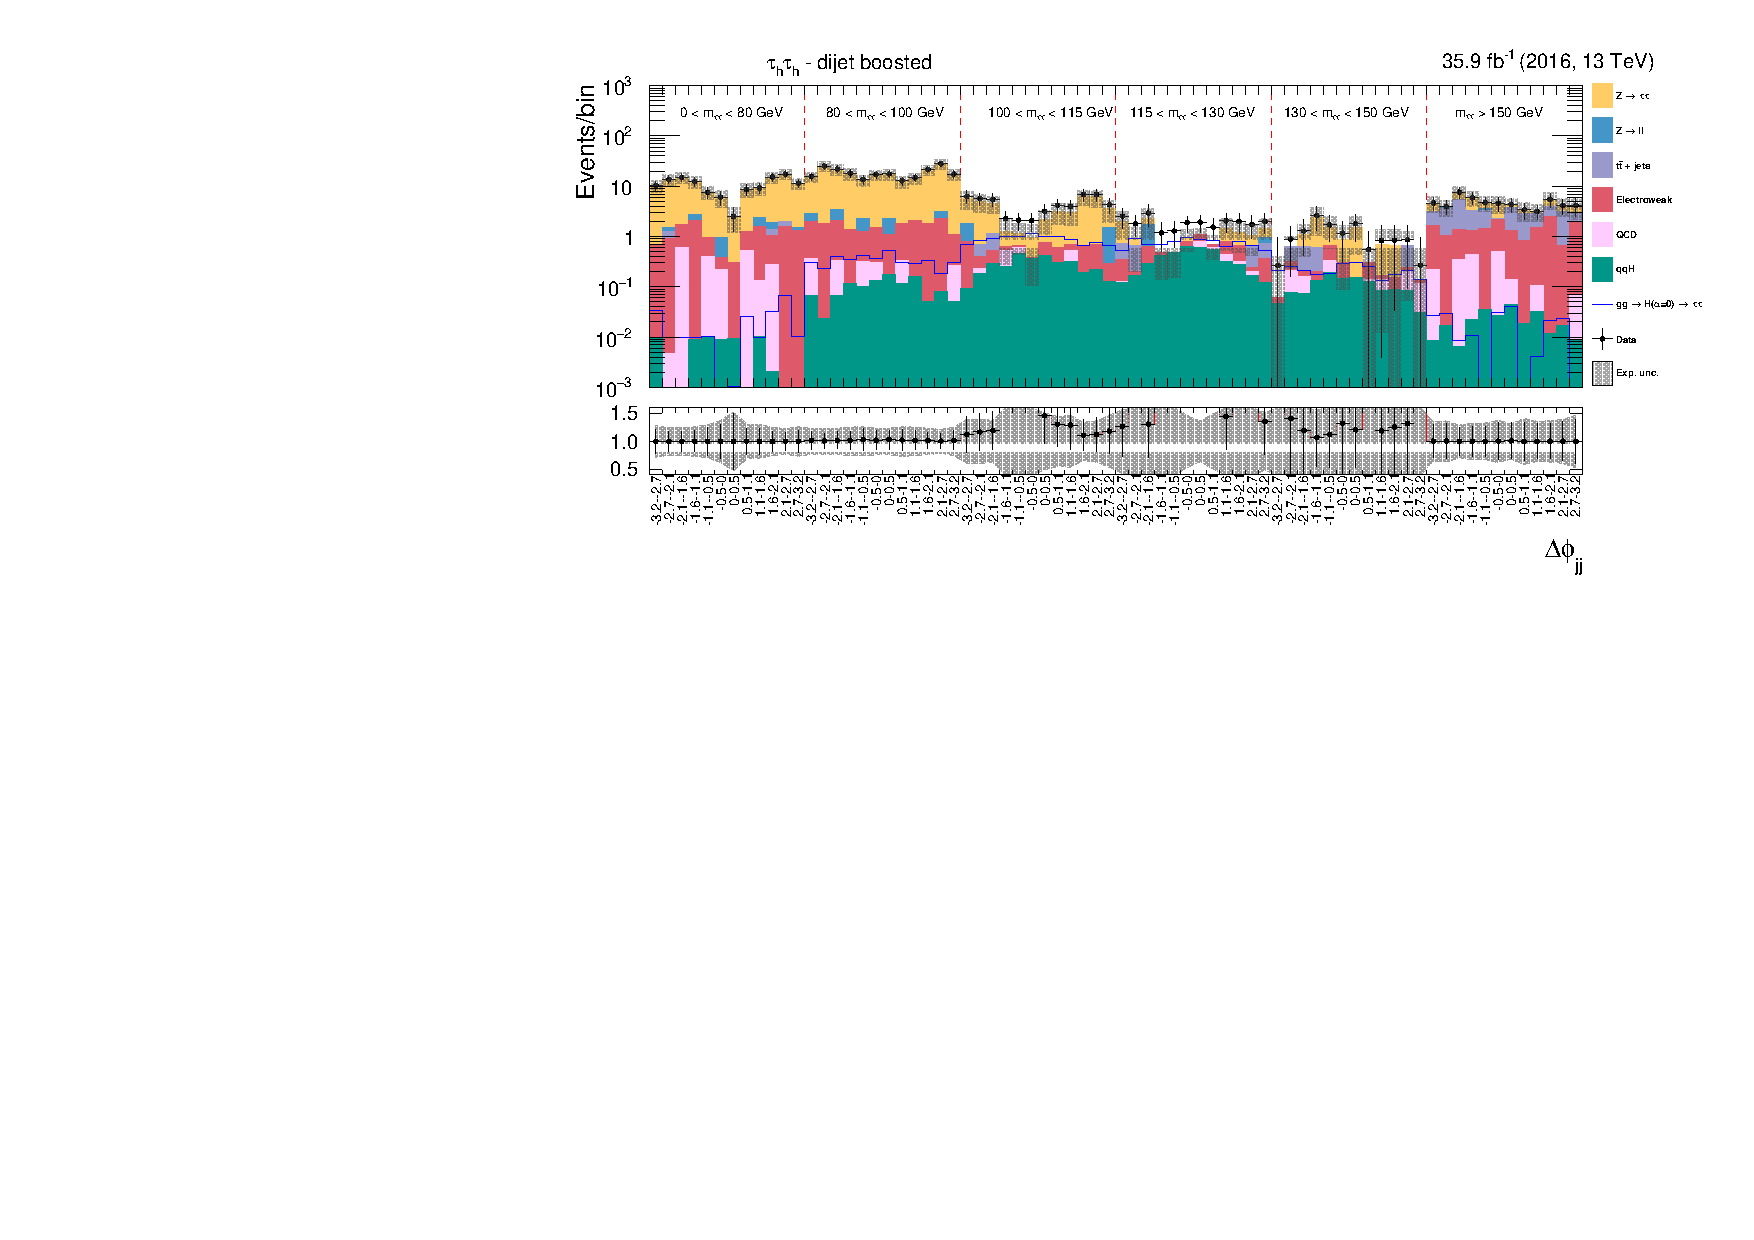
\includegraphics[width=\textwidth]{Figures/statana/Postfit_JEC_jdphi/prefit_htt_tt_4_13TeV.pdf}         
    \caption{Prefit distributions of the \textit{dijet lowboost} and \textit{dijet boosted} categories in the \tautau{} channel  using \jdphi{}.}
\end{figure}
\clearpage
\begin{figure}[h!]
    \centering
        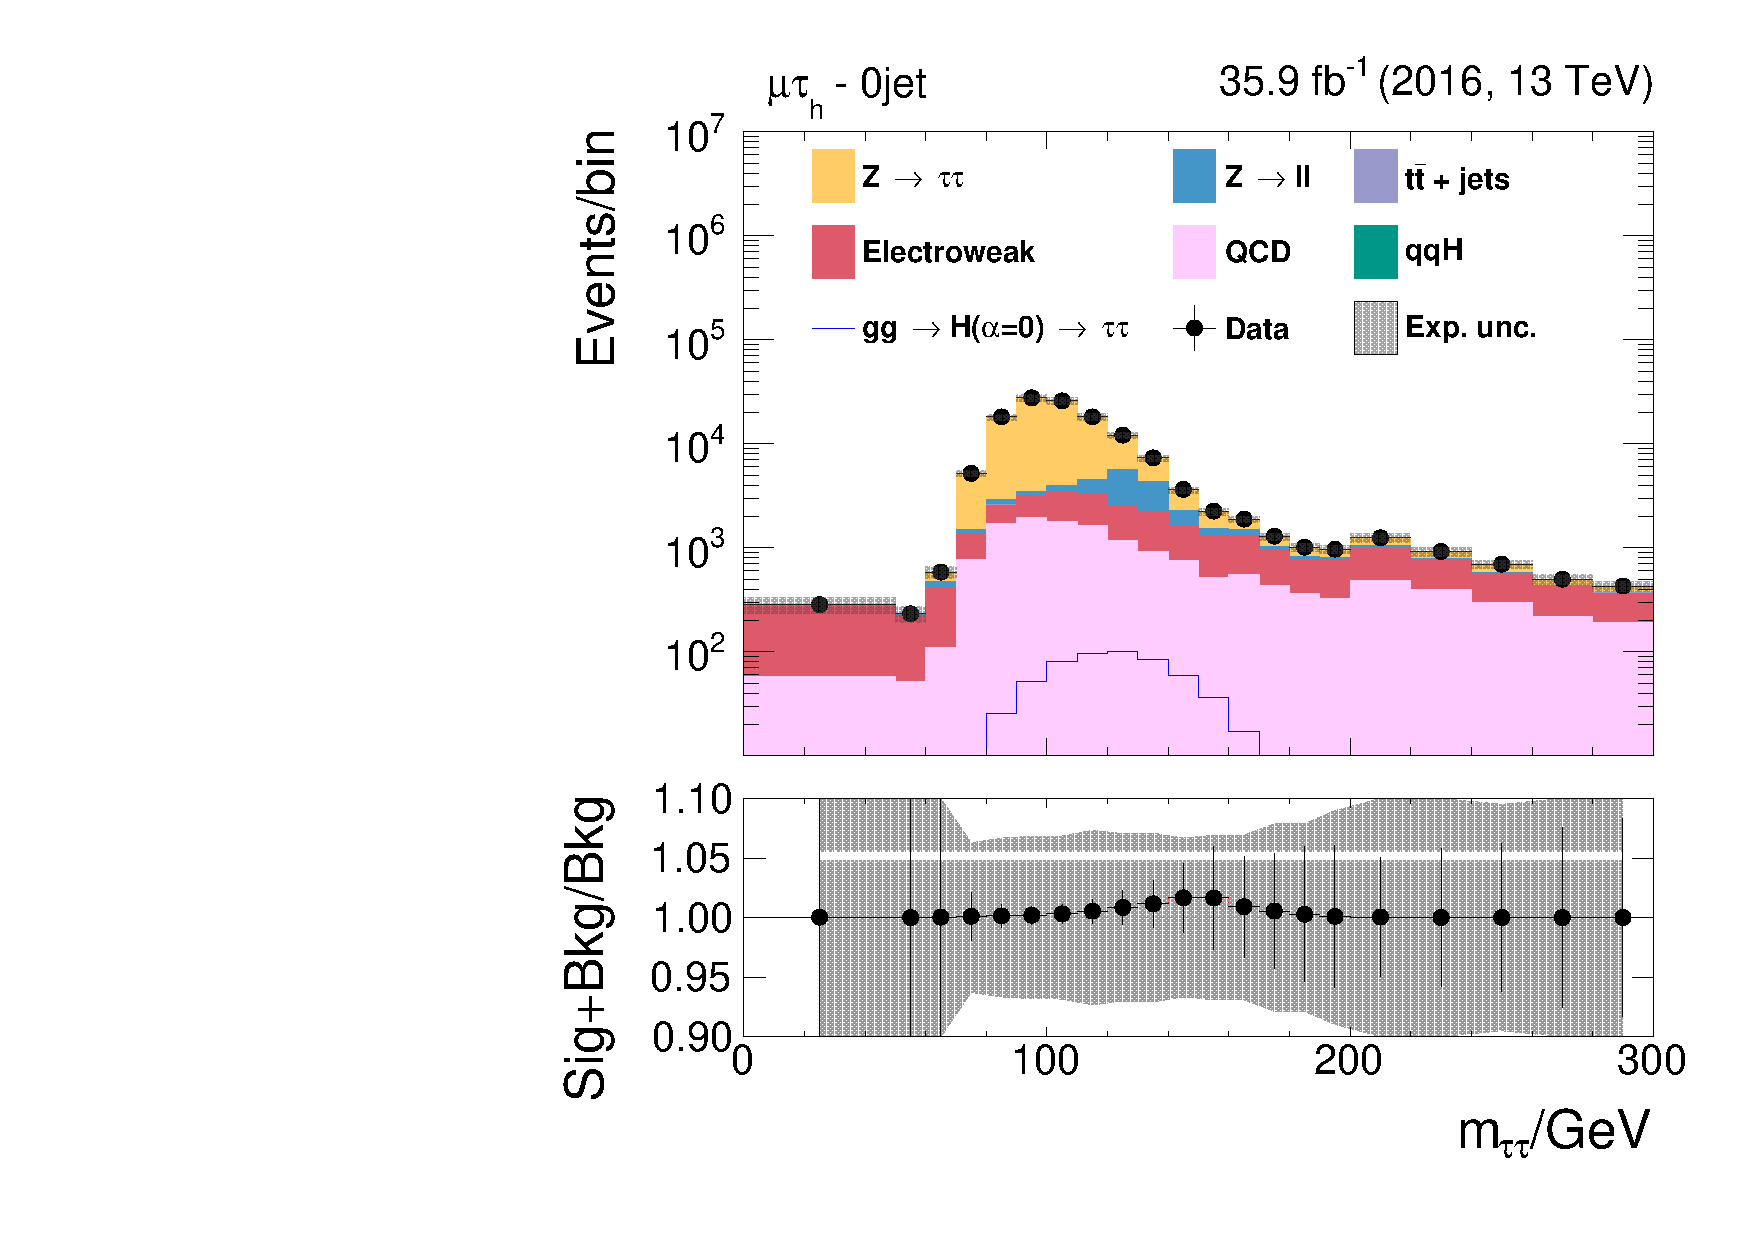
\includegraphics[width=.5\textwidth]{Figures/statana/Postfit_JEC_jdphi/prefit_htt_mt_1_13TeV.pdf}\\
        \includegraphics[width=\textwidth]{Figures/statana/Postfit_JEC_jdphi/prefit_htt_mt_2_13TeV.pdf}
        \caption{Prefit distributions of the \textit{0-jet} and \textit{boosted} categories in the \mutau{} channel  using \jdphi{}.}
    \end{figure}
    \begin{figure}[h!]
        \centering        
        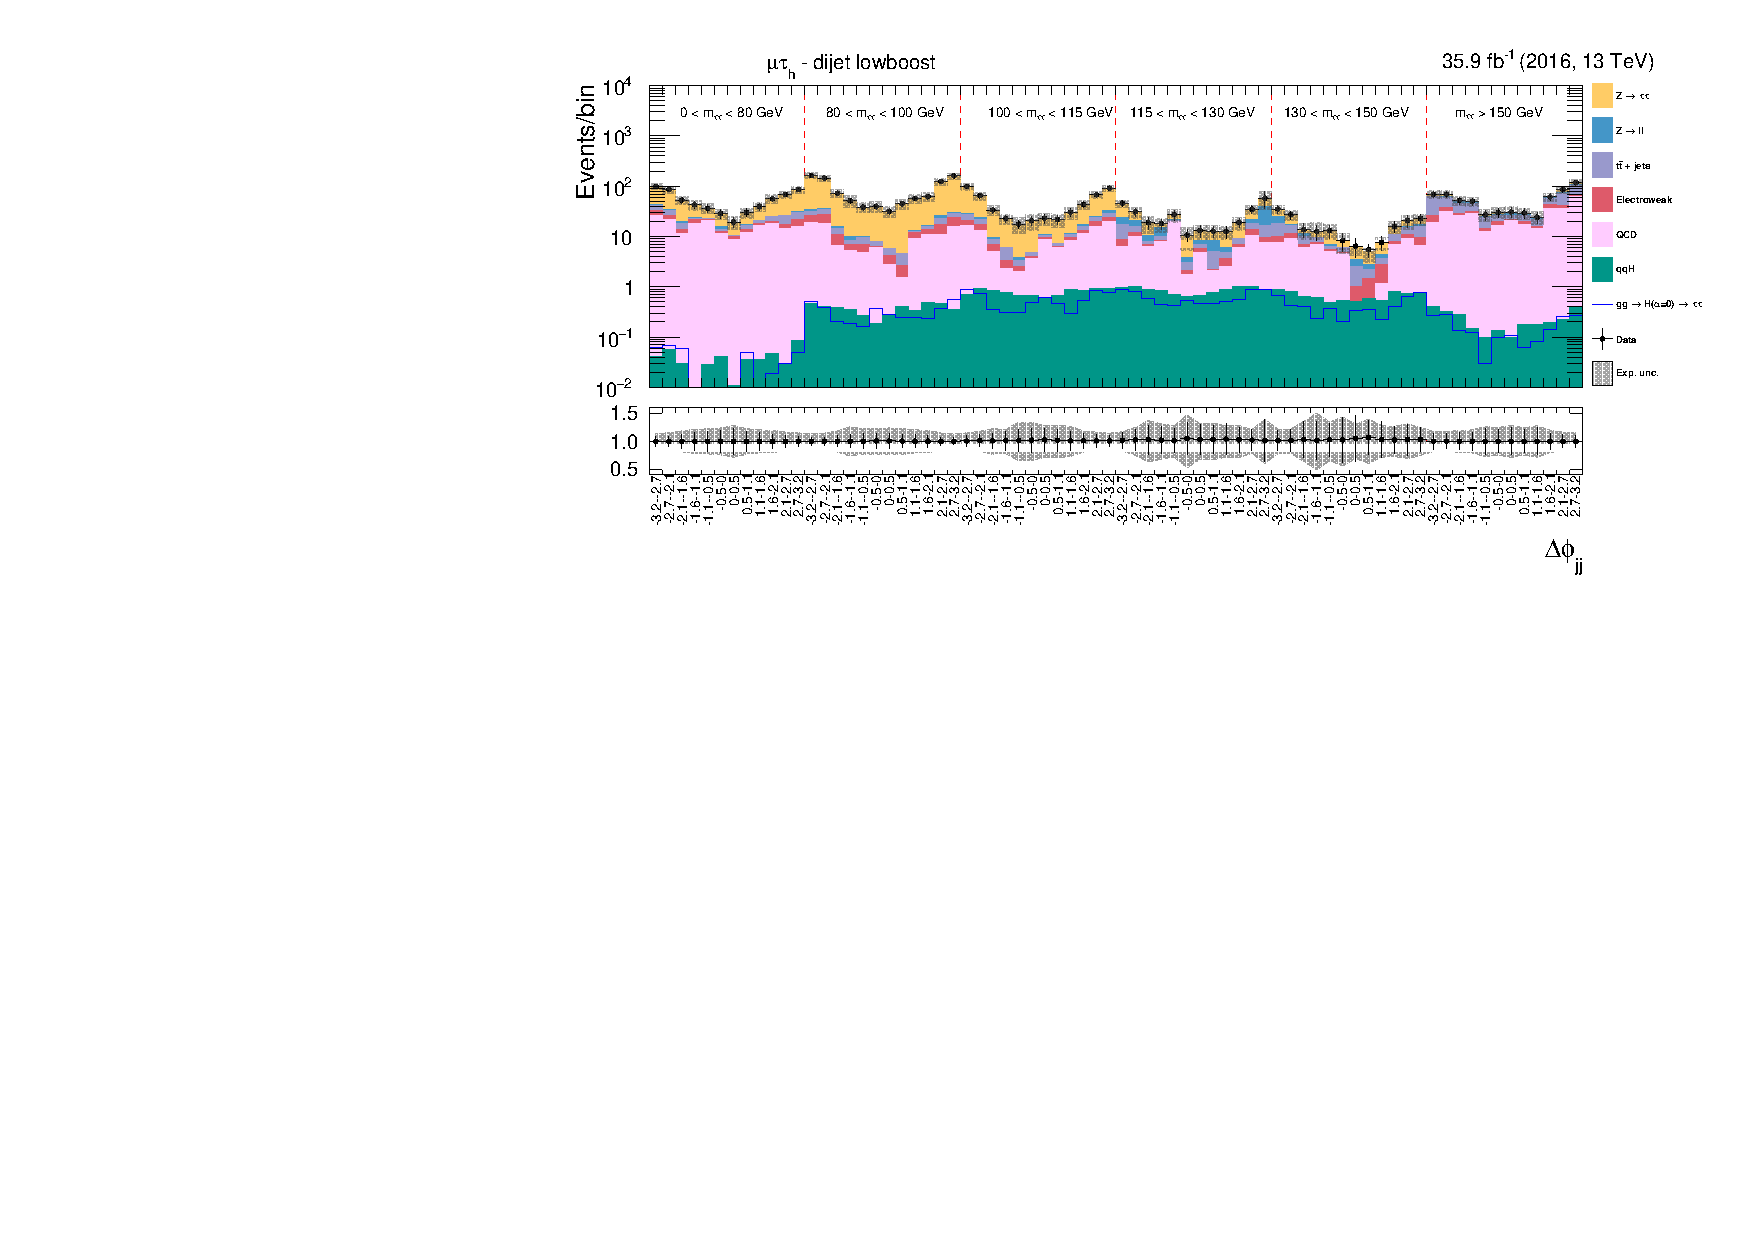
\includegraphics[width=\textwidth]{Figures/statana/Postfit_JEC_jdphi/prefit_htt_mt_3_13TeV.pdf}\\
        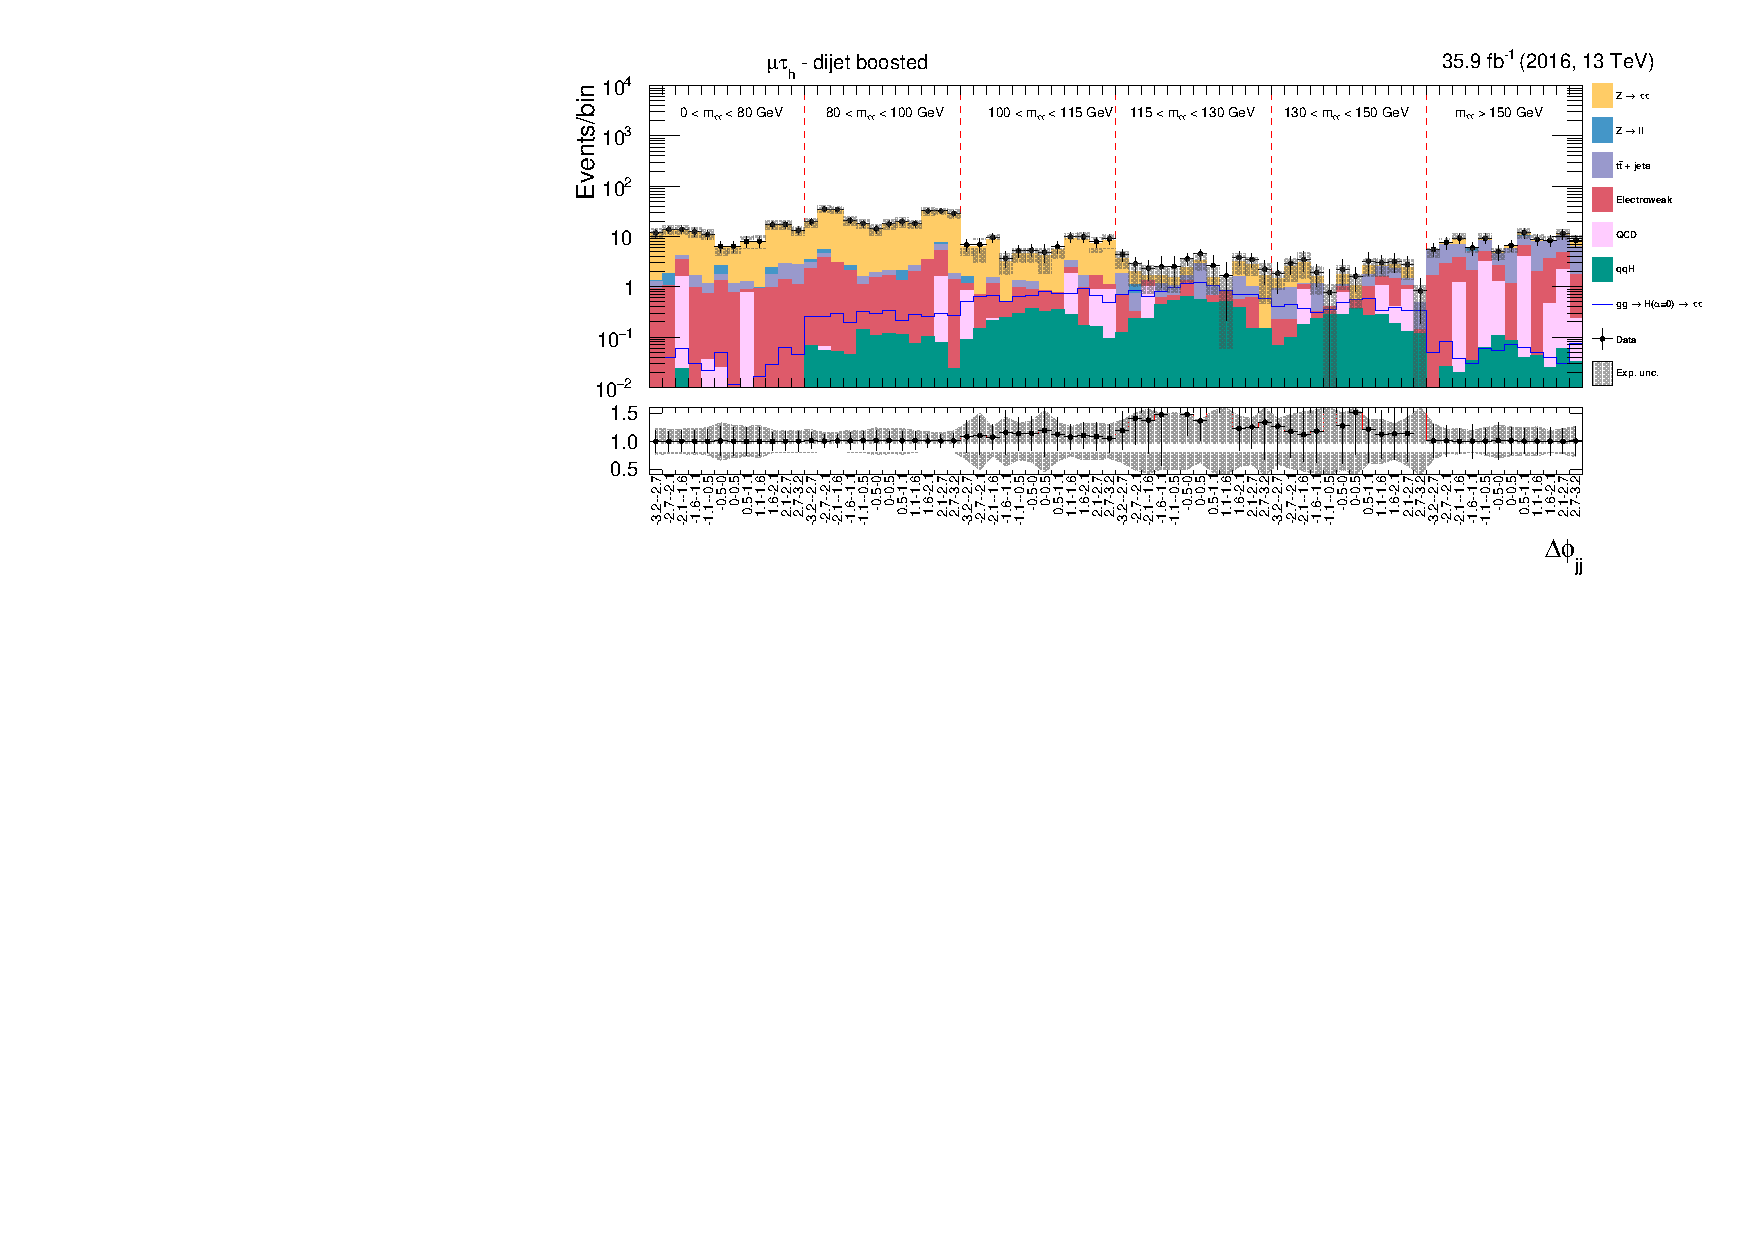
\includegraphics[width=\textwidth]{Figures/statana/Postfit_JEC_jdphi/prefit_htt_mt_4_13TeV.pdf}
    \caption{Prefit distributions of the \textit{dijet lowboost} and \textit{dijet boosted} categories in the \mutau{} channel  using \jdphi{}.}
\end{figure}
\clearpage
\begin{figure}[h!]
    \centering
        \includegraphics[width=.5\textwidth]{Figures/statana/Postfit_JEC_jdphi/prefit_htt_et_1_13TeV.pdf}\\
        \includegraphics[width=\textwidth]{Figures/statana/Postfit_JEC_jdphi/prefit_htt_et_2_13TeV.pdf}
    \caption{Prefit distributions of the \textit{0-jet} and \textit{boosted} categories in the \etau{} channel  using \jdphi{}.}
\end{figure}  
\begin{figure}[h!]
    \centering      
        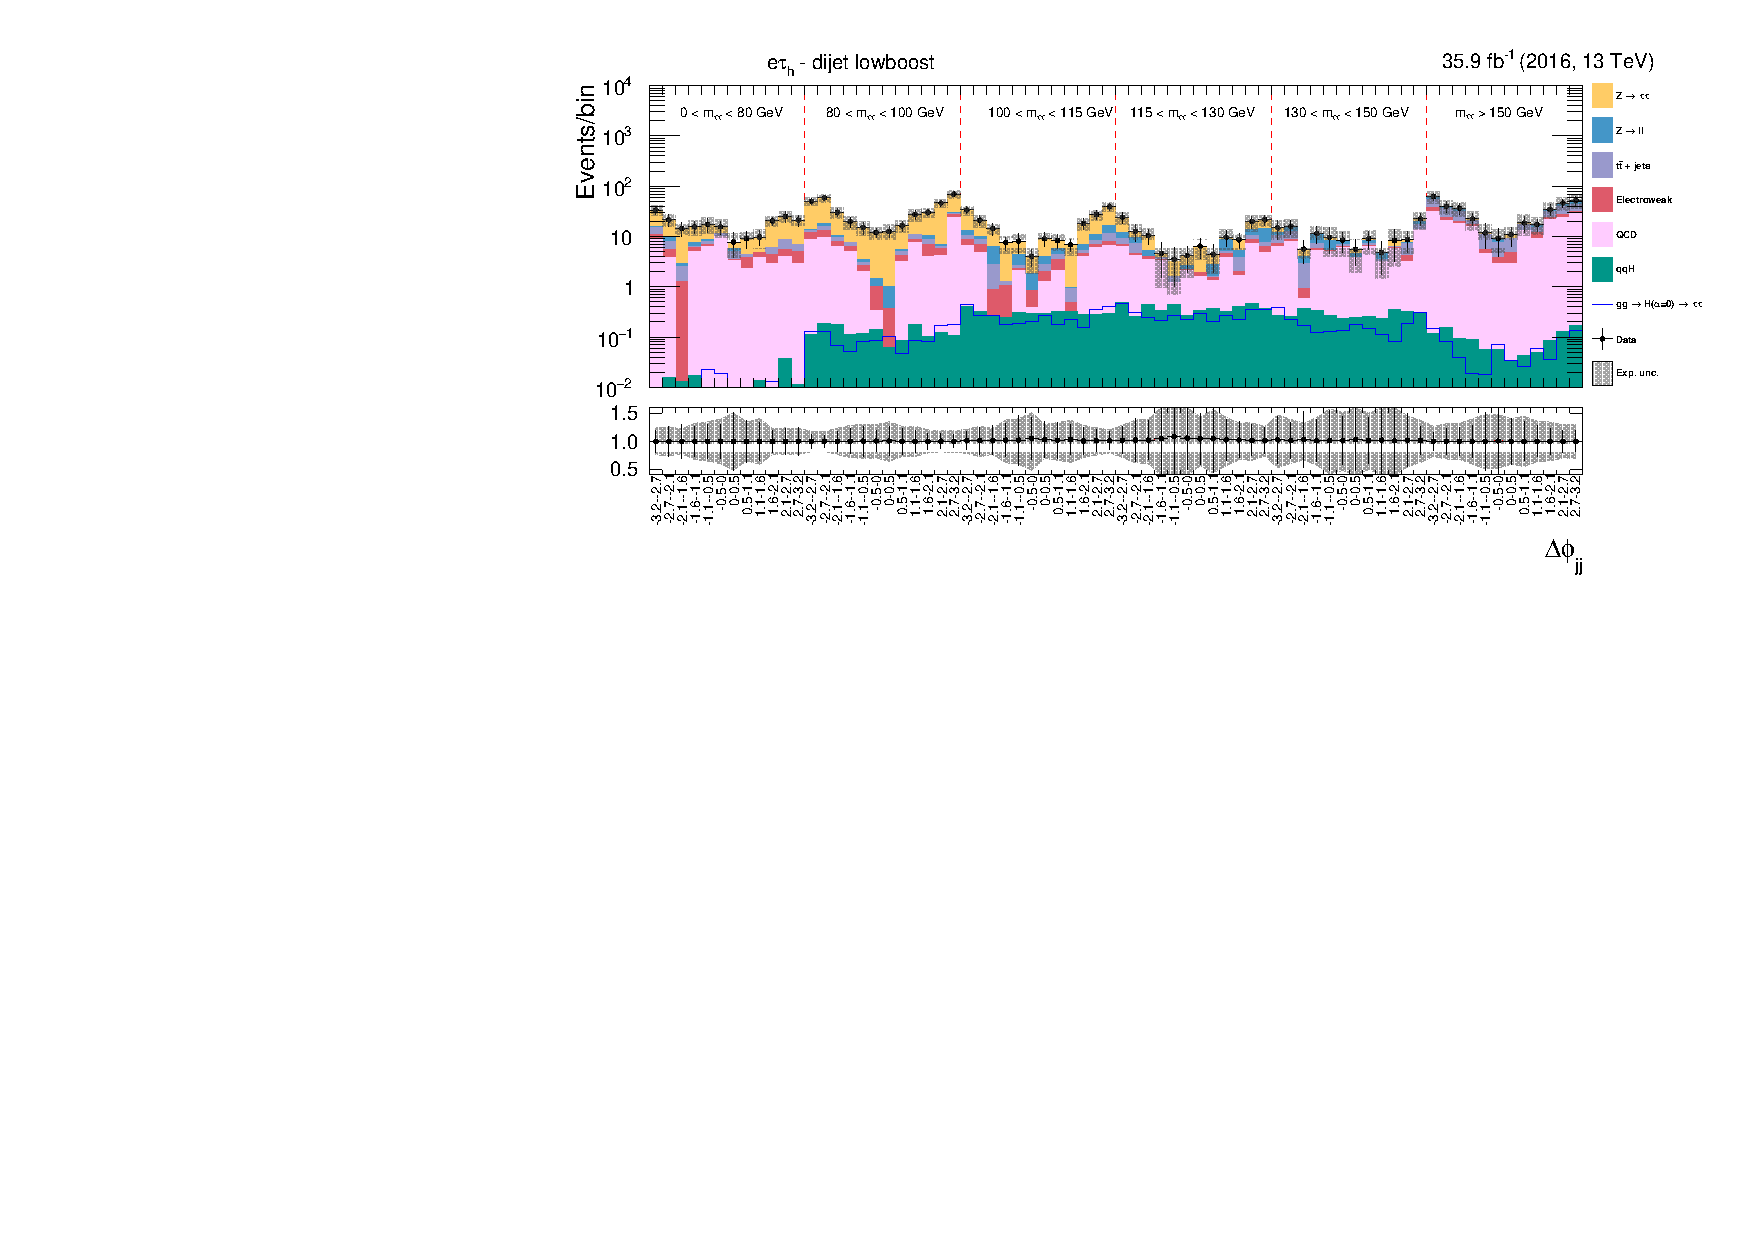
\includegraphics[width=\textwidth]{Figures/statana/Postfit_JEC_jdphi/prefit_htt_et_3_13TeV.pdf}\\
        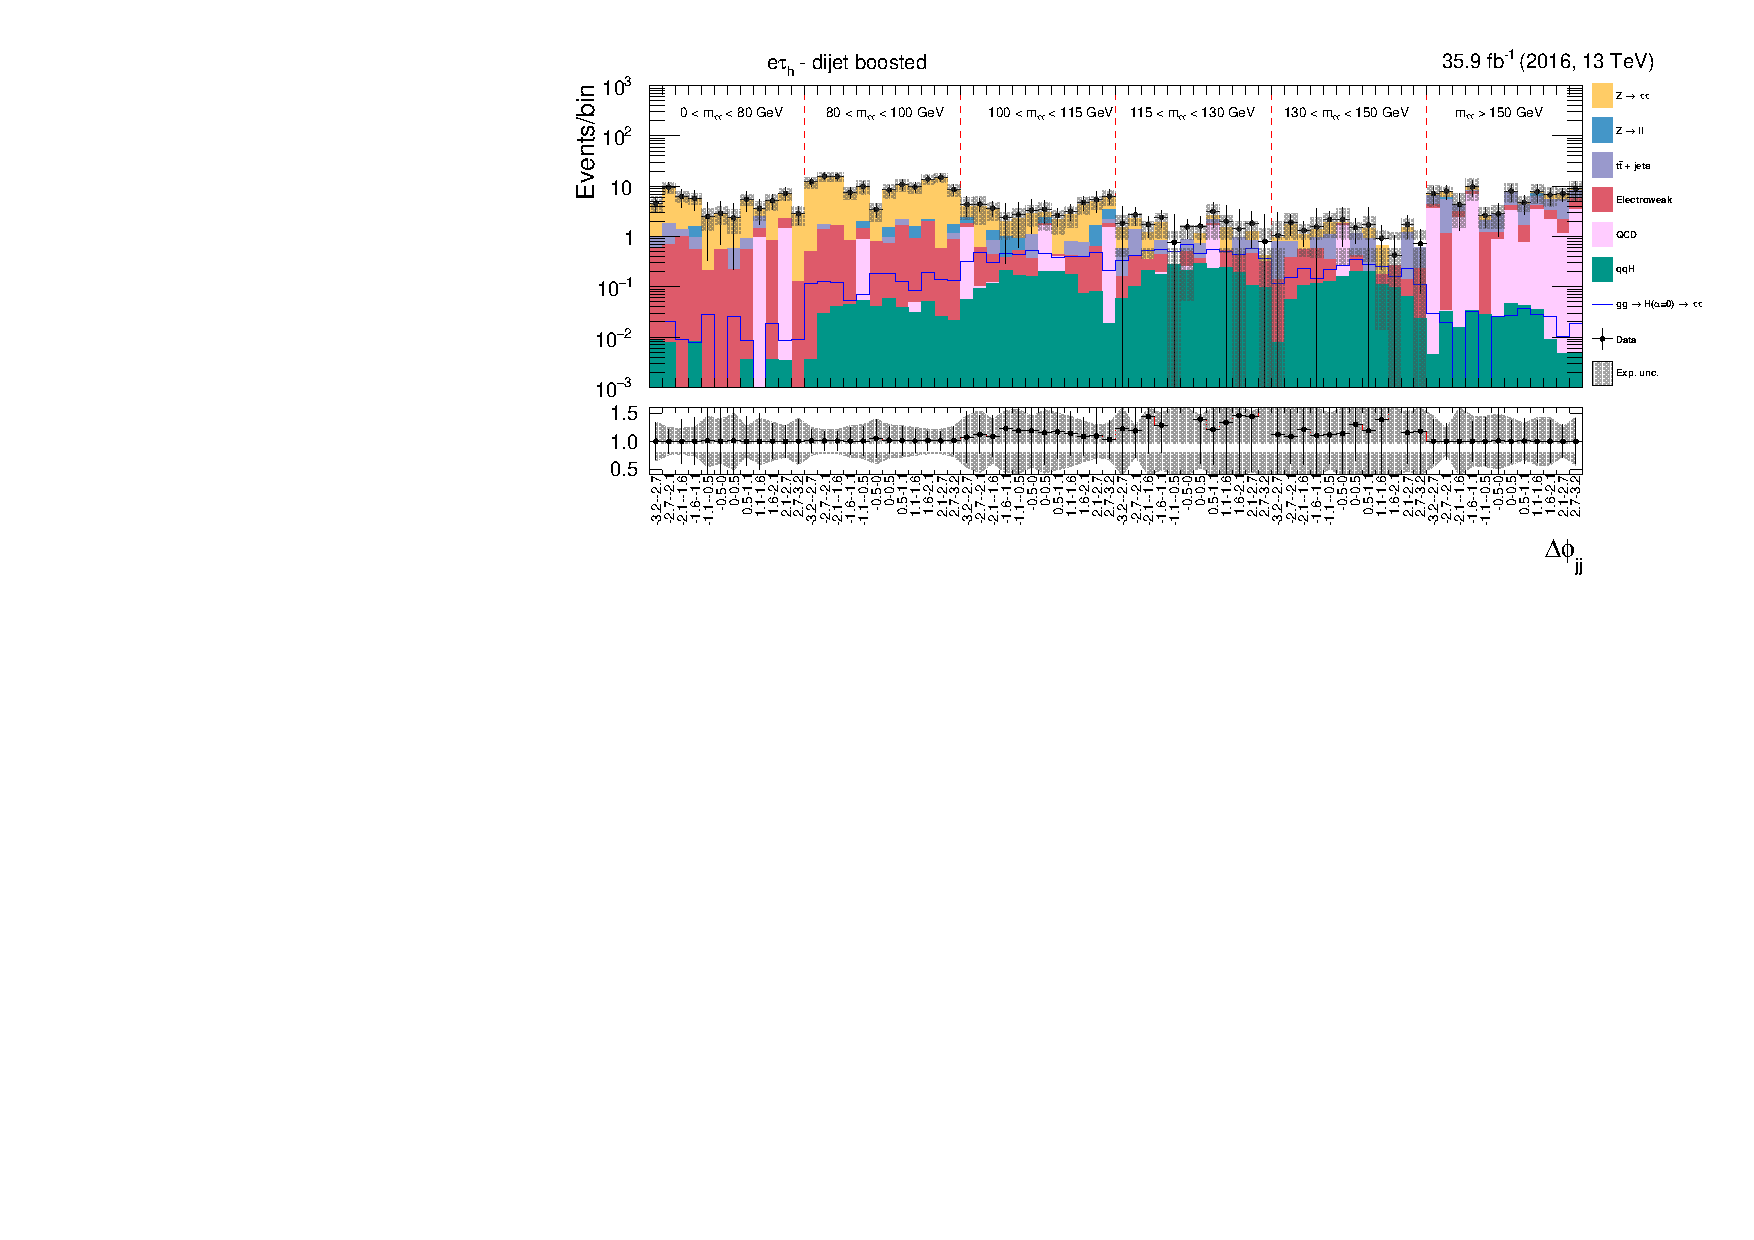
\includegraphics[width=\textwidth]{Figures/statana/Postfit_JEC_jdphi/prefit_htt_et_4_13TeV.pdf}
    \caption{Prefit distributions of the \textit{dijet lowboost} and \textit{dijet boosted} categories in the \etau{} channel  using \jdphi{}.}
\end{figure}
\clearpage
\begin{figure}[h!]
    \centering
        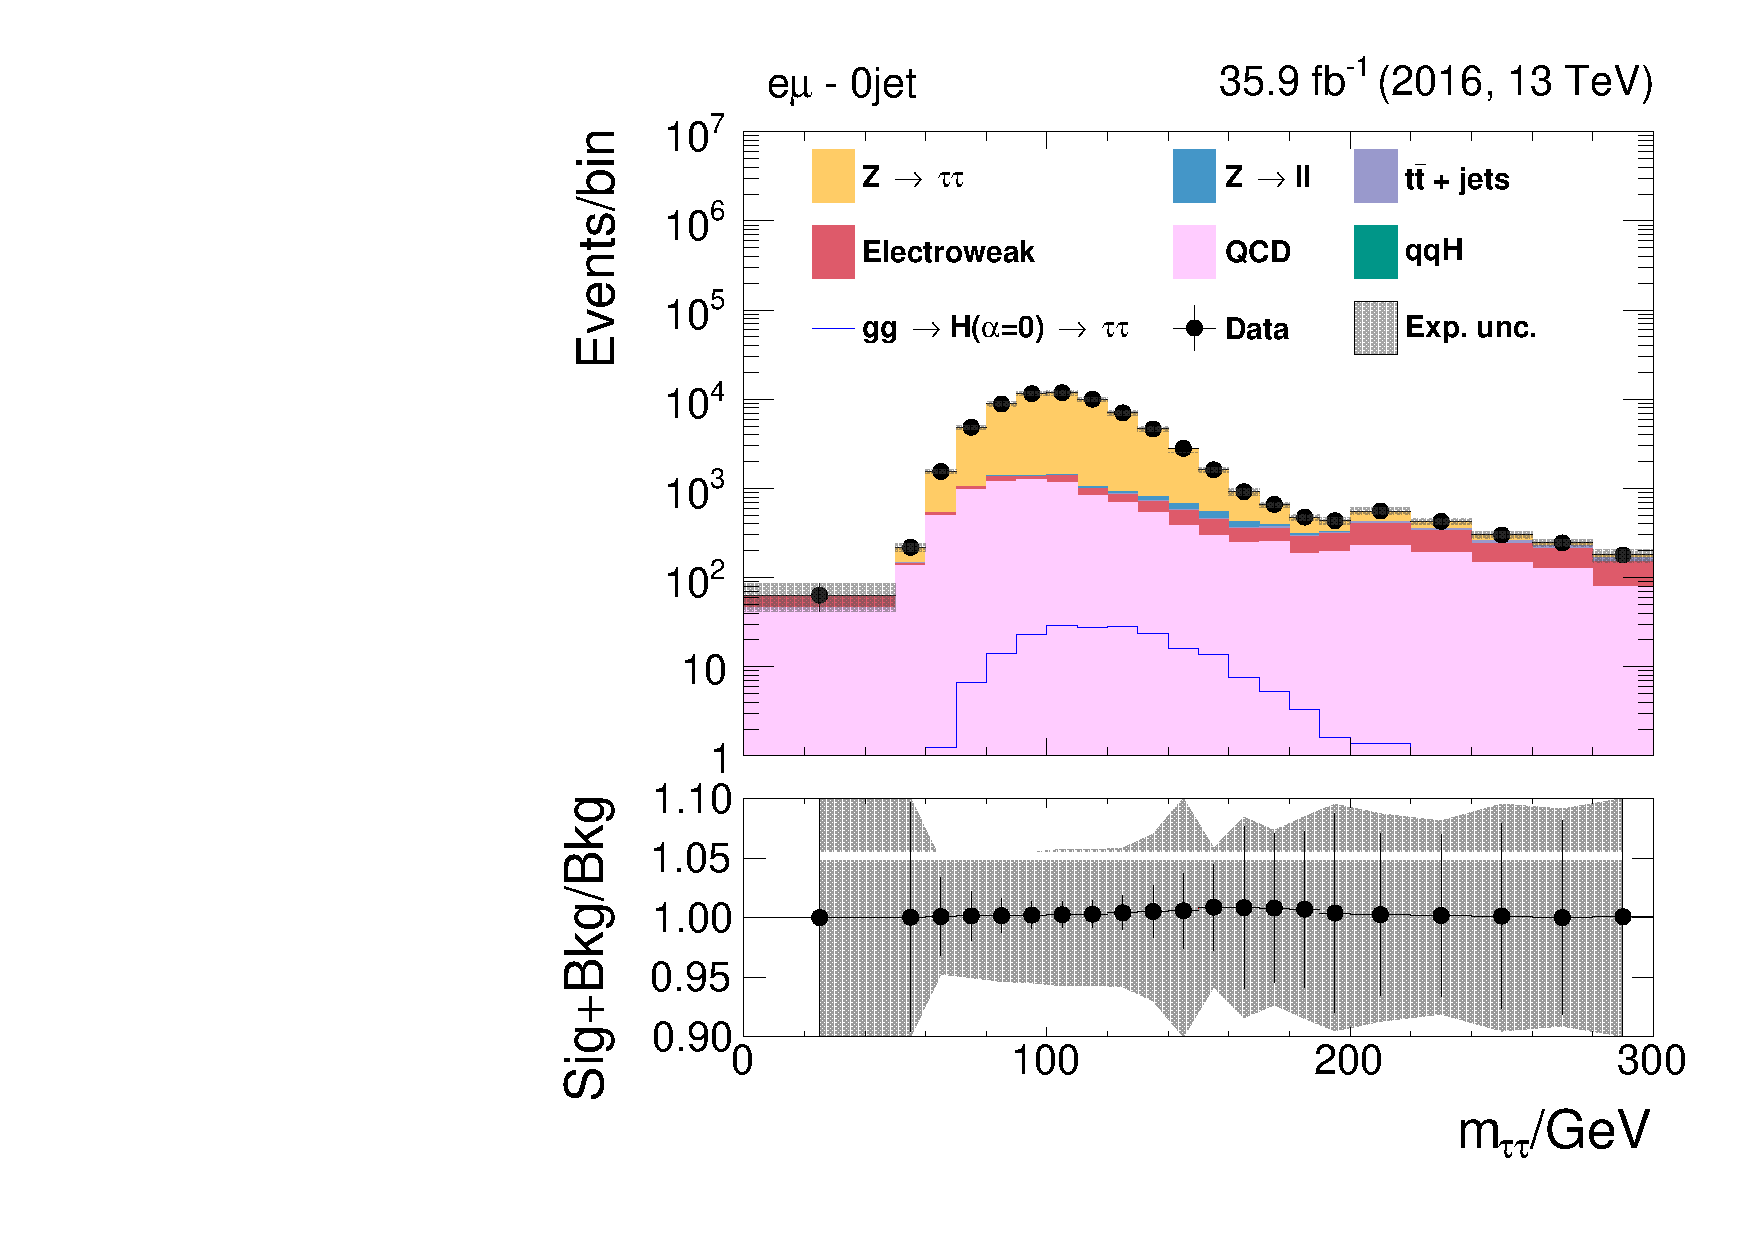
\includegraphics[width=.5\textwidth]{Figures/statana/Postfit_JEC_jdphi/prefit_htt_em_1_13TeV.pdf}\\
        \includegraphics[width=\textwidth]{Figures/statana/Postfit_JEC_jdphi/prefit_htt_em_2_13TeV.pdf}
    \caption{Prefit distributions of the \textit{0-jet} and \textit{boosted} categories in the \emu{} channel using \jdphi{}.}
\end{figure} 
\begin{figure}[h!]
    \centering       
        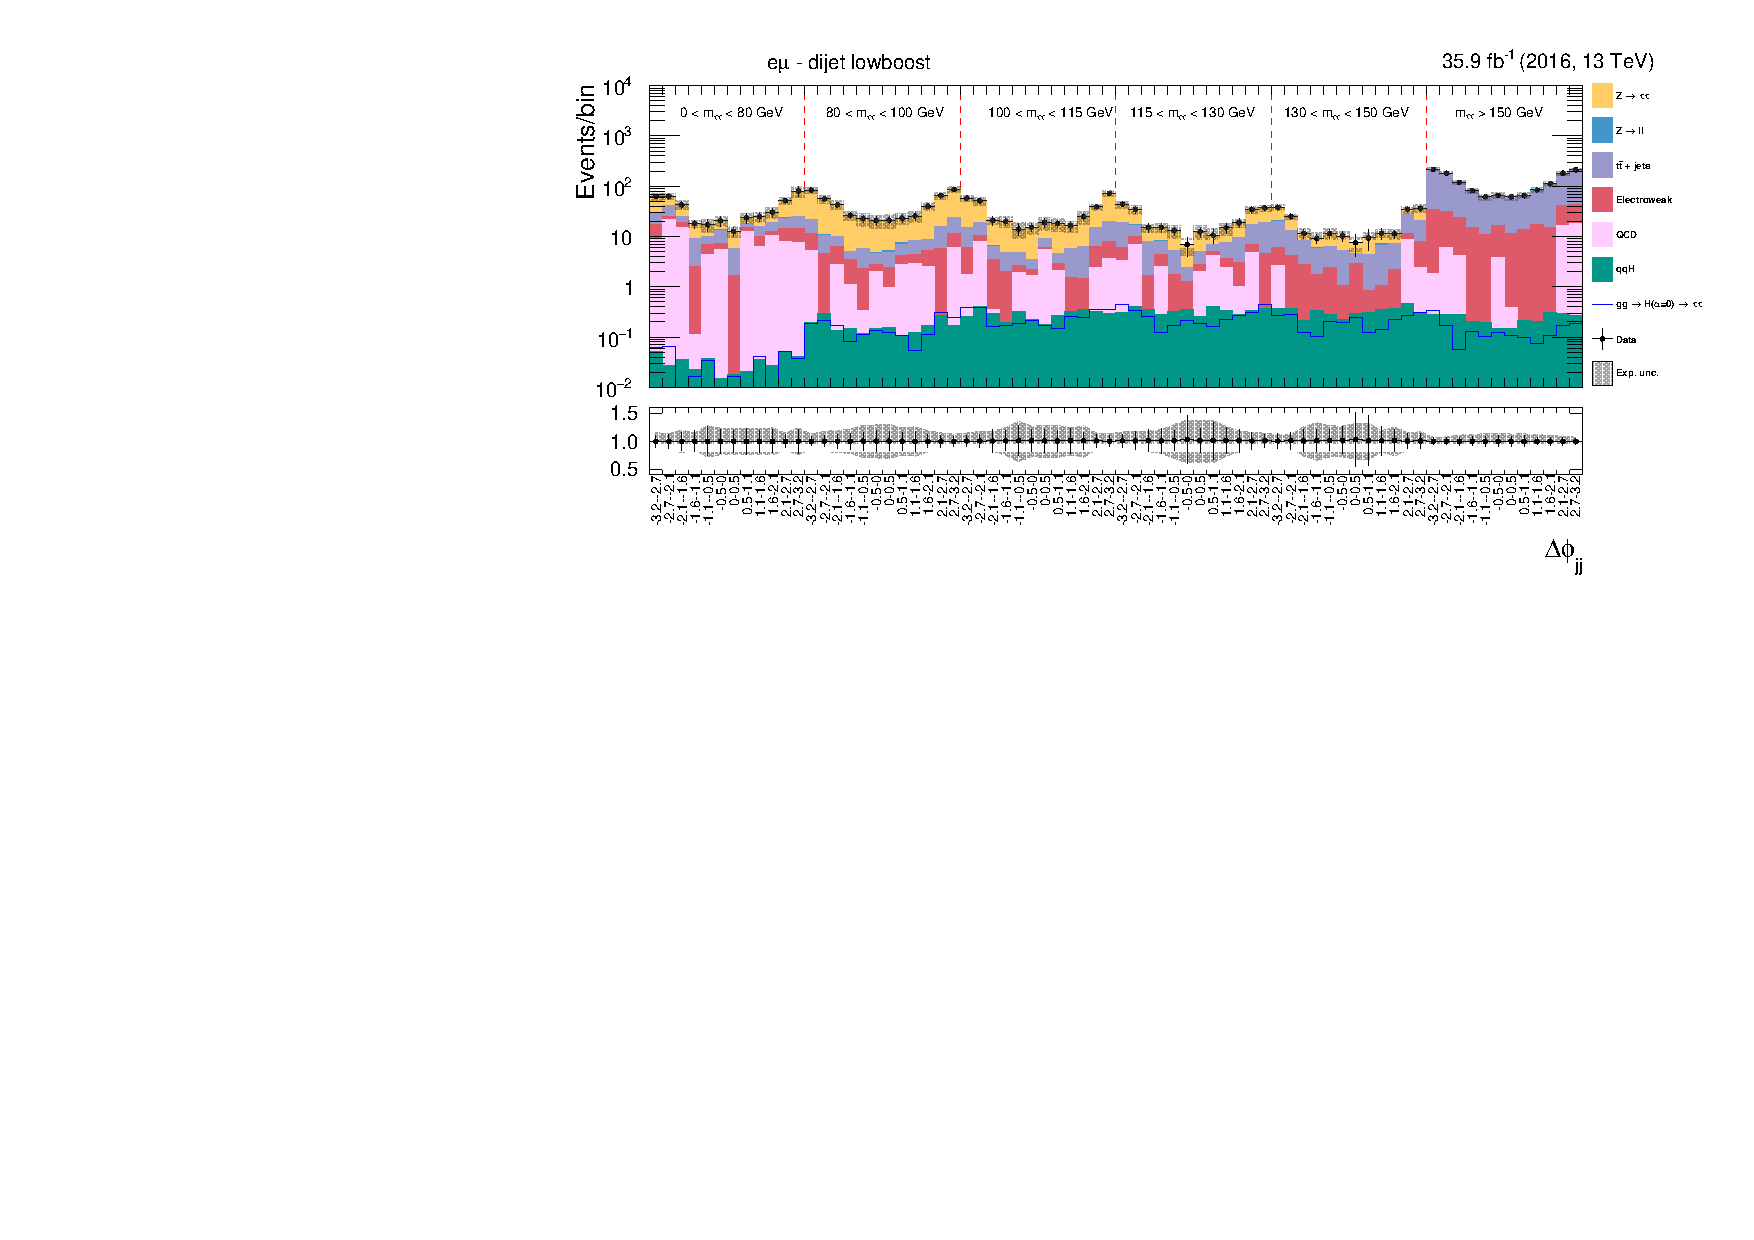
\includegraphics[width=\textwidth]{Figures/statana/Postfit_JEC_jdphi/prefit_htt_em_3_13TeV.pdf}\\
        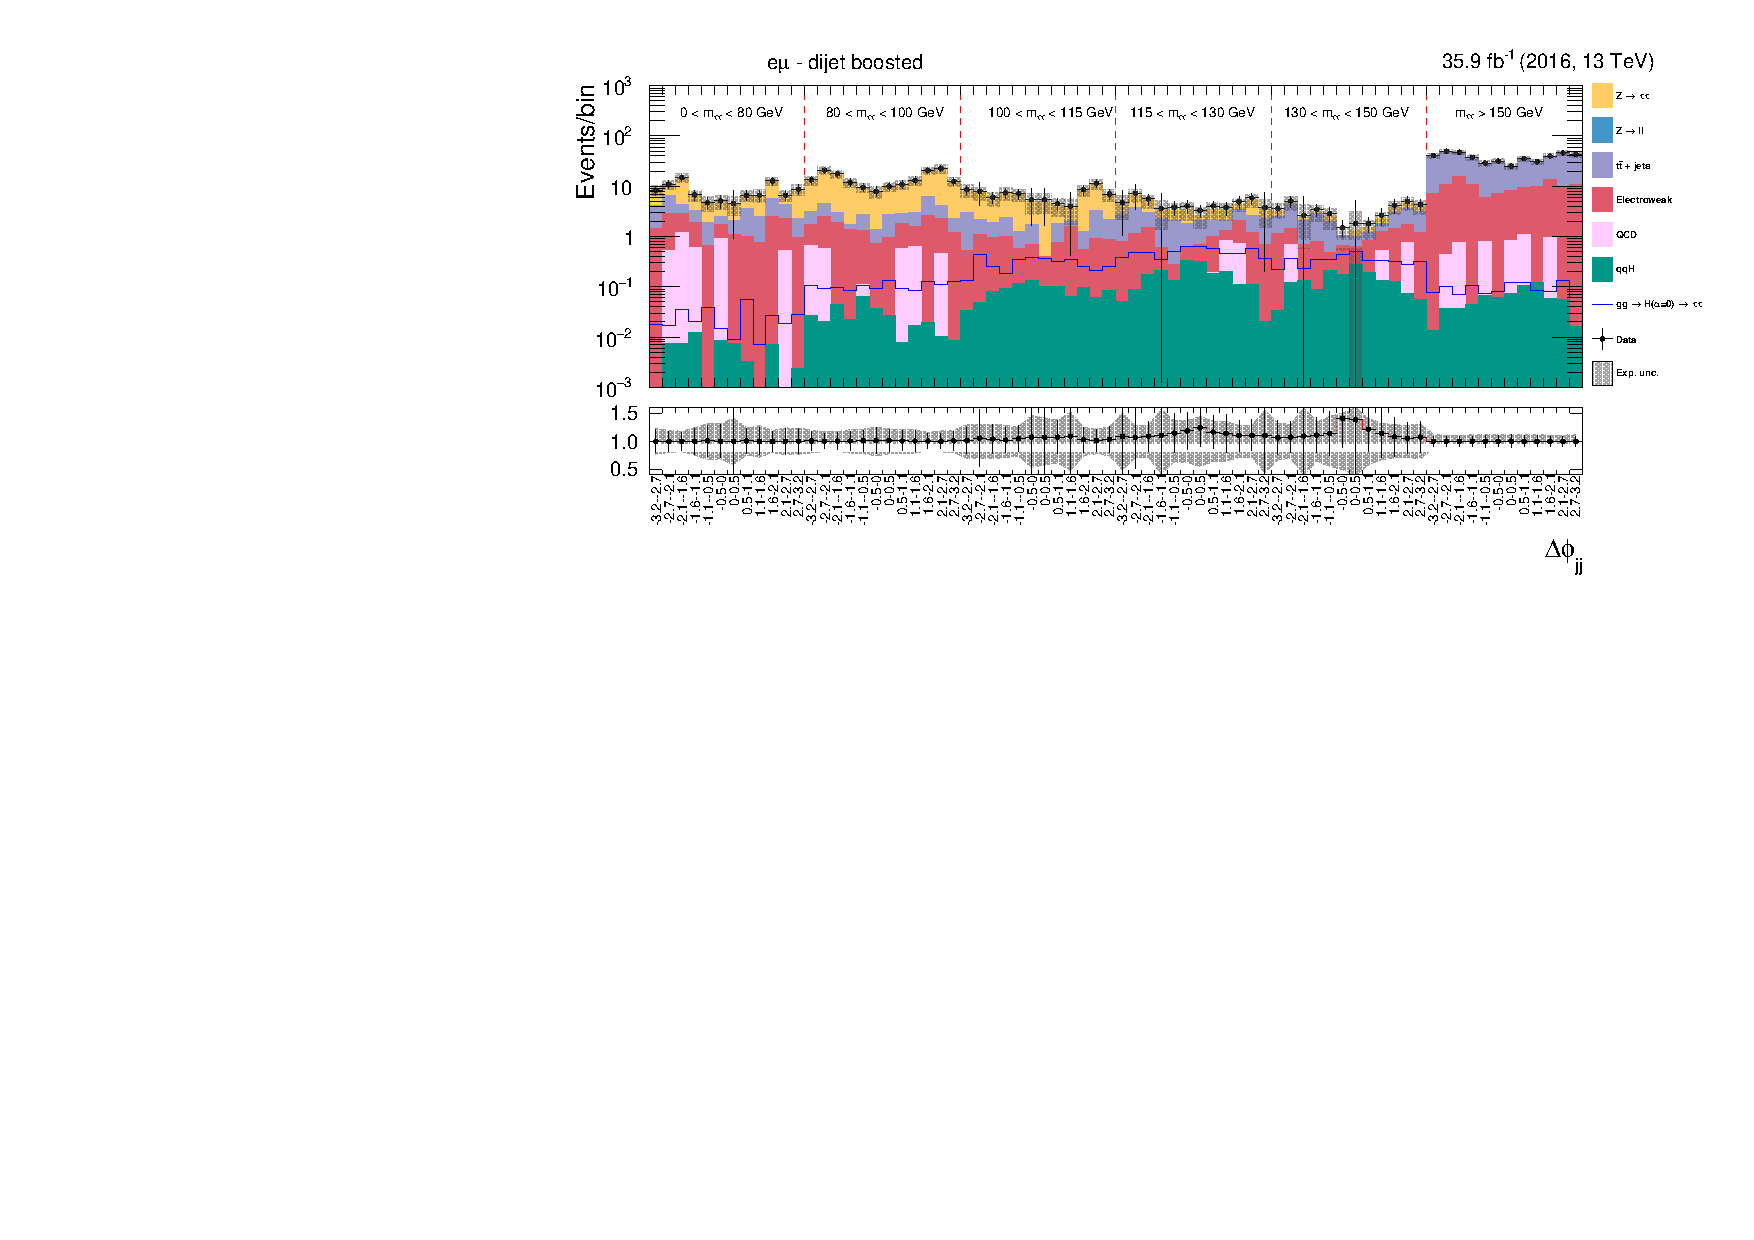
\includegraphics[width=\textwidth]{Figures/statana/Postfit_JEC_jdphi/prefit_htt_em_4_13TeV.pdf}
    \caption{Prefit distributions of the \textit{dijet lowboost} and \textit{dijet boosted} categories in the \emu{} channel  using \jdphi{}.}
\end{figure}
\clearpage

\subsection{Postfit distributions for \jdphi}

\begin{figure}[h!]
    \centering
        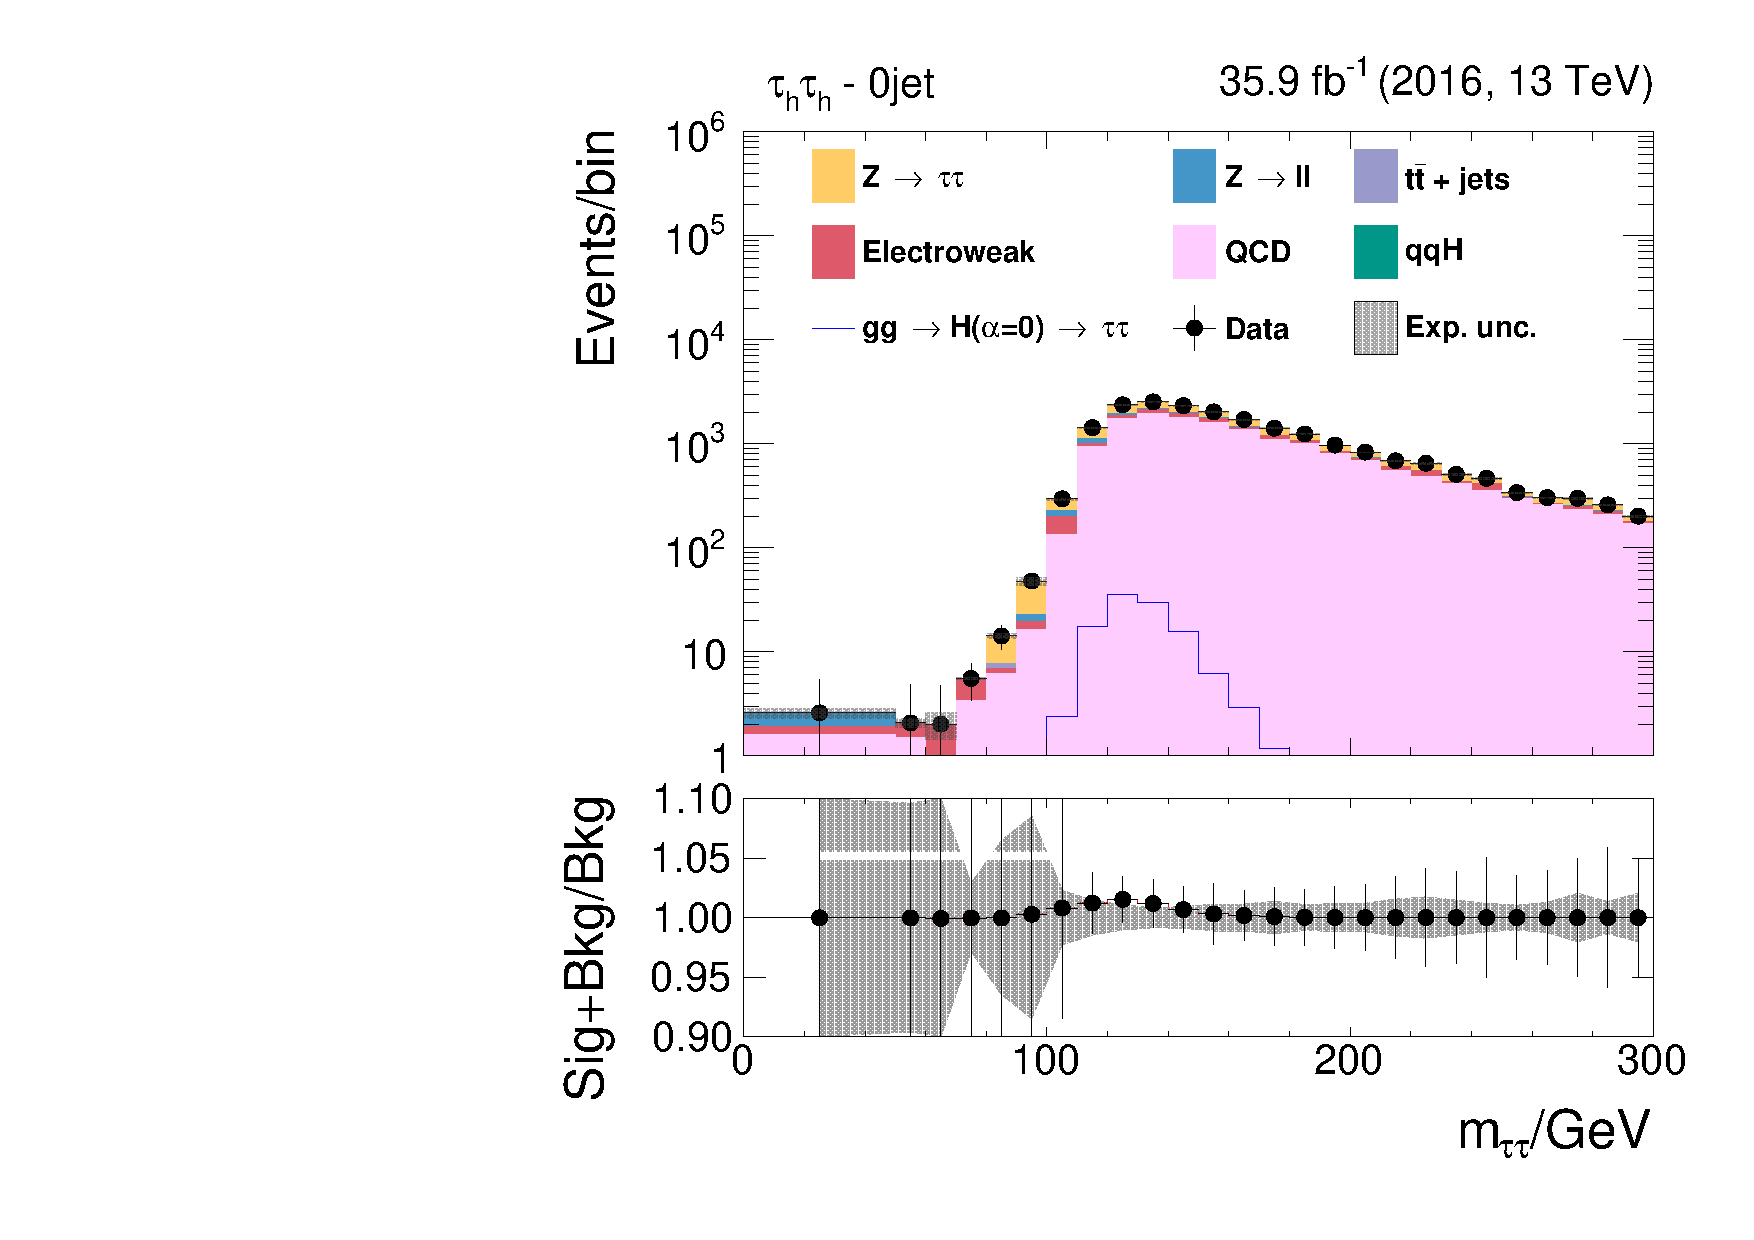
\includegraphics[width=.5\textwidth]{Figures/statana/Postfit_JEC_jdphi/postfit_fit_s_htt_tt_1_13TeV.pdf}\\
        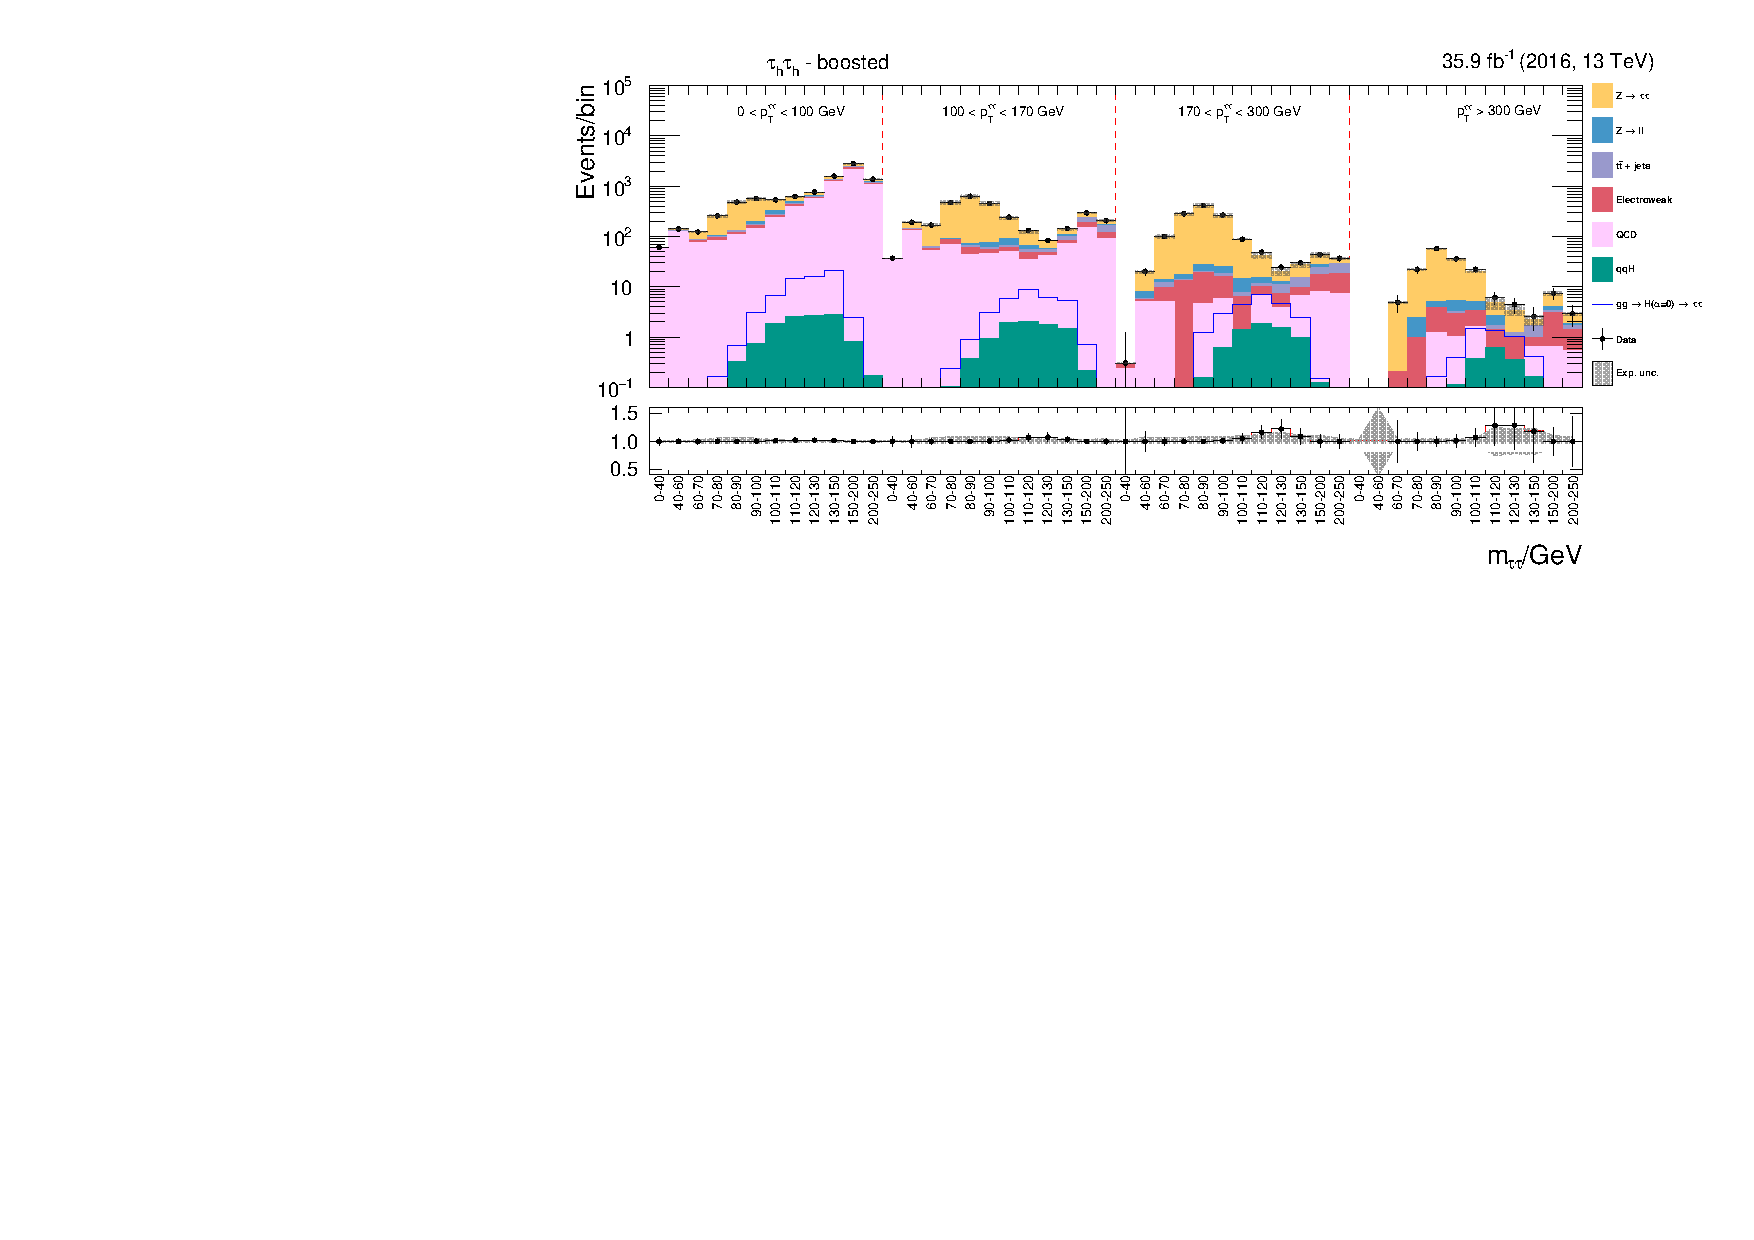
\includegraphics[width=\textwidth]{Figures/statana/Postfit_JEC_jdphi/postfit_fit_s_htt_tt_2_13TeV.pdf}    
    \caption{Postfit distributions of the \textit{0-jet} and \textit{boosted} categories in the \tautau{} channel  using \jdphi{}.}
\end{figure}
\begin{figure}[h!]
    \centering
        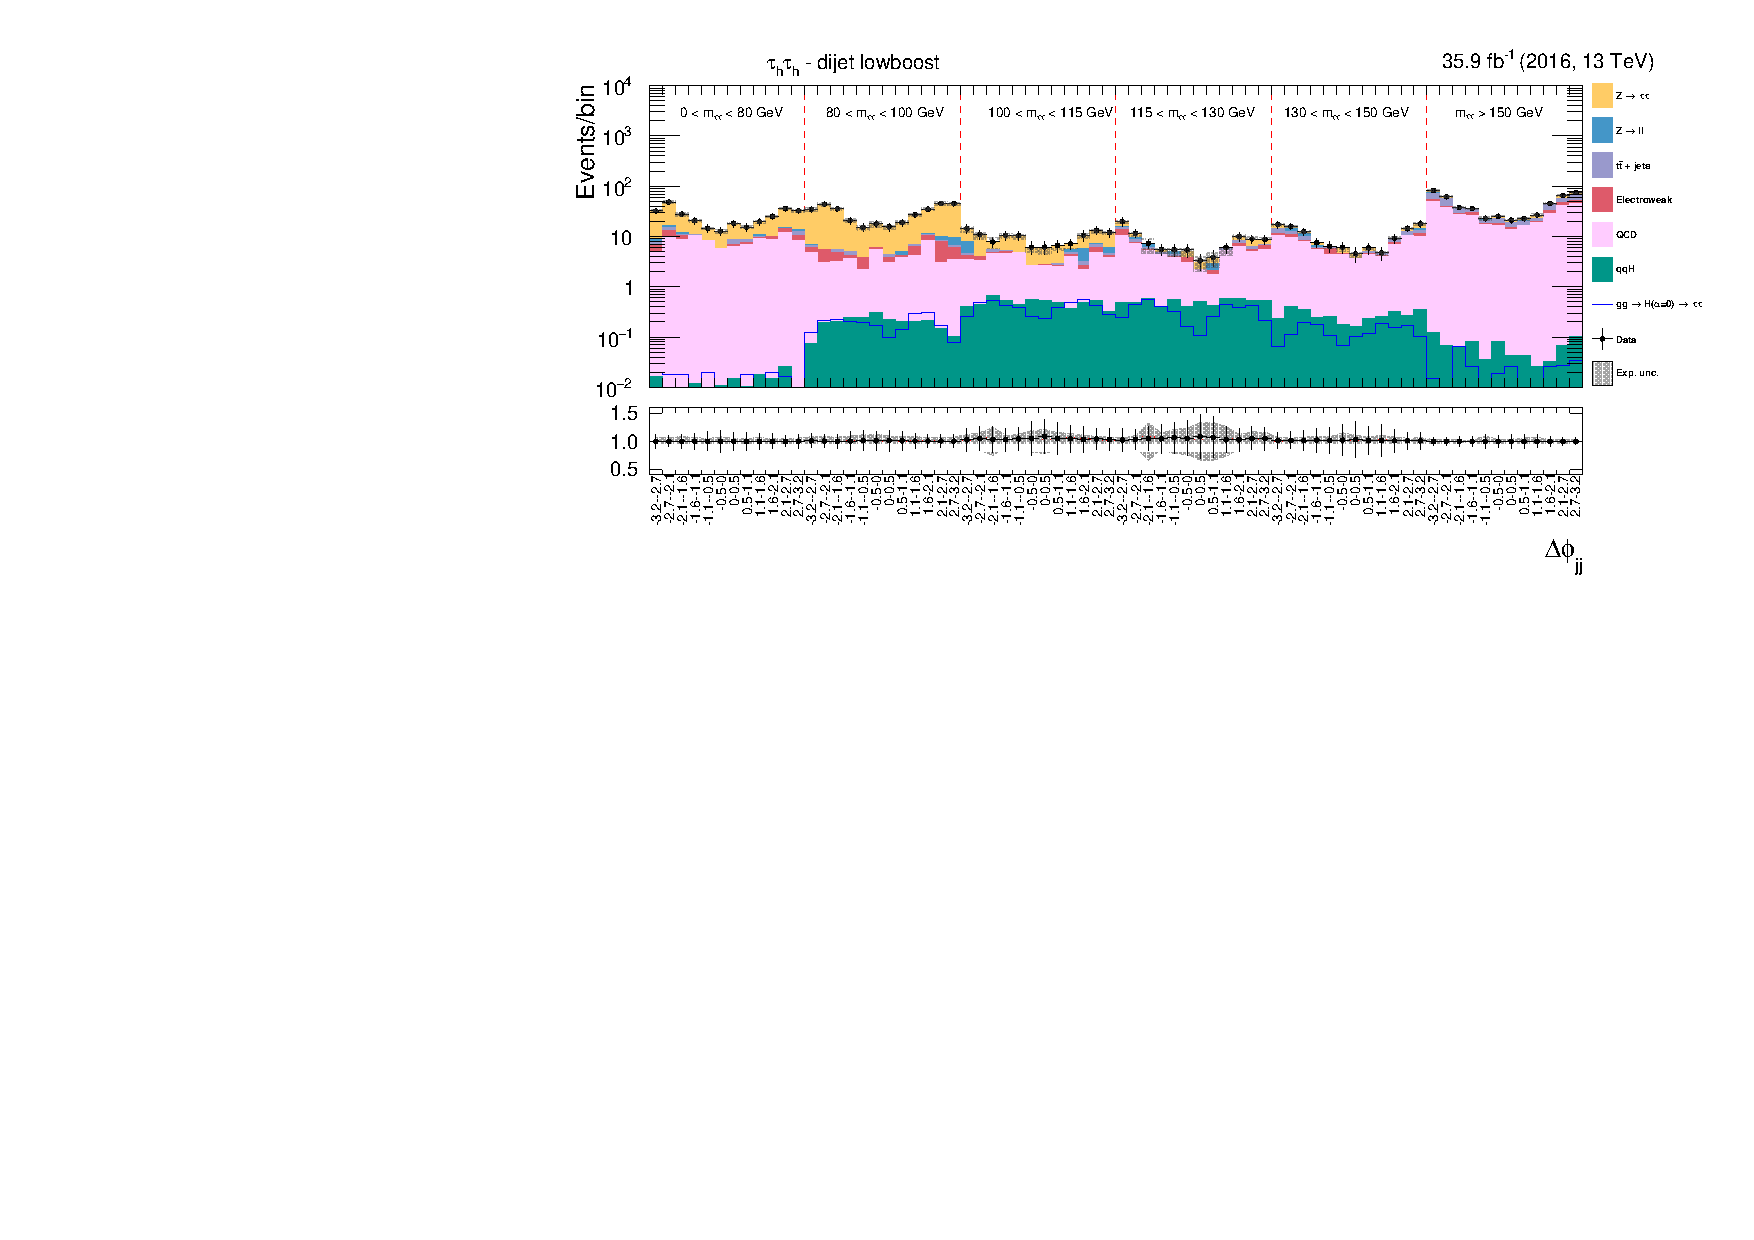
\includegraphics[width=\textwidth]{Figures/statana/Postfit_JEC_jdphi/postfit_fit_s_htt_tt_3_13TeV.pdf}\\
        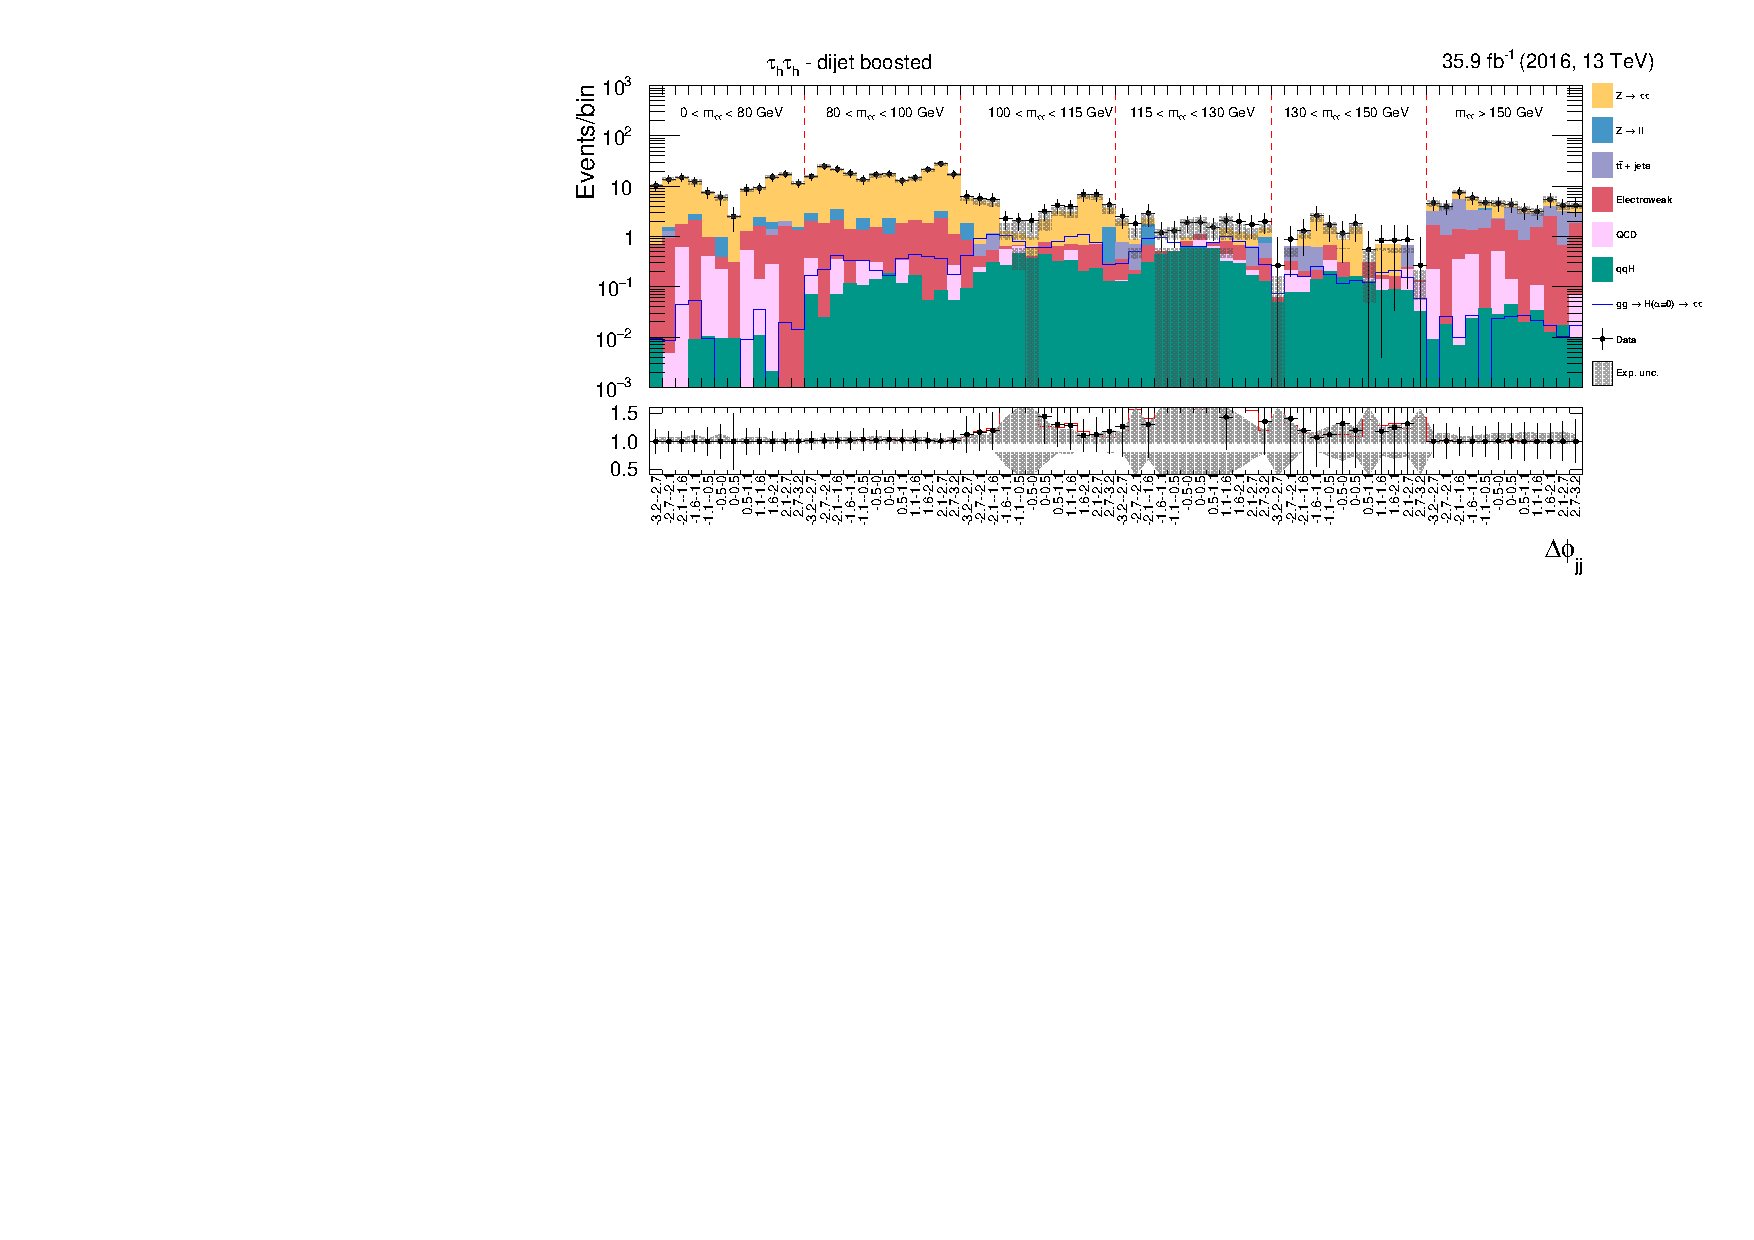
\includegraphics[width=\textwidth]{Figures/statana/Postfit_JEC_jdphi/postfit_fit_s_htt_tt_4_13TeV.pdf}
    \caption{Postfit distributions of the \textit{dijet lowboost} and \textit{dijet boosted} categories in the \tautau{} channel  using \jdphi{}.}
\end{figure}
\clearpage
\begin{figure}[h!]
    \centering
        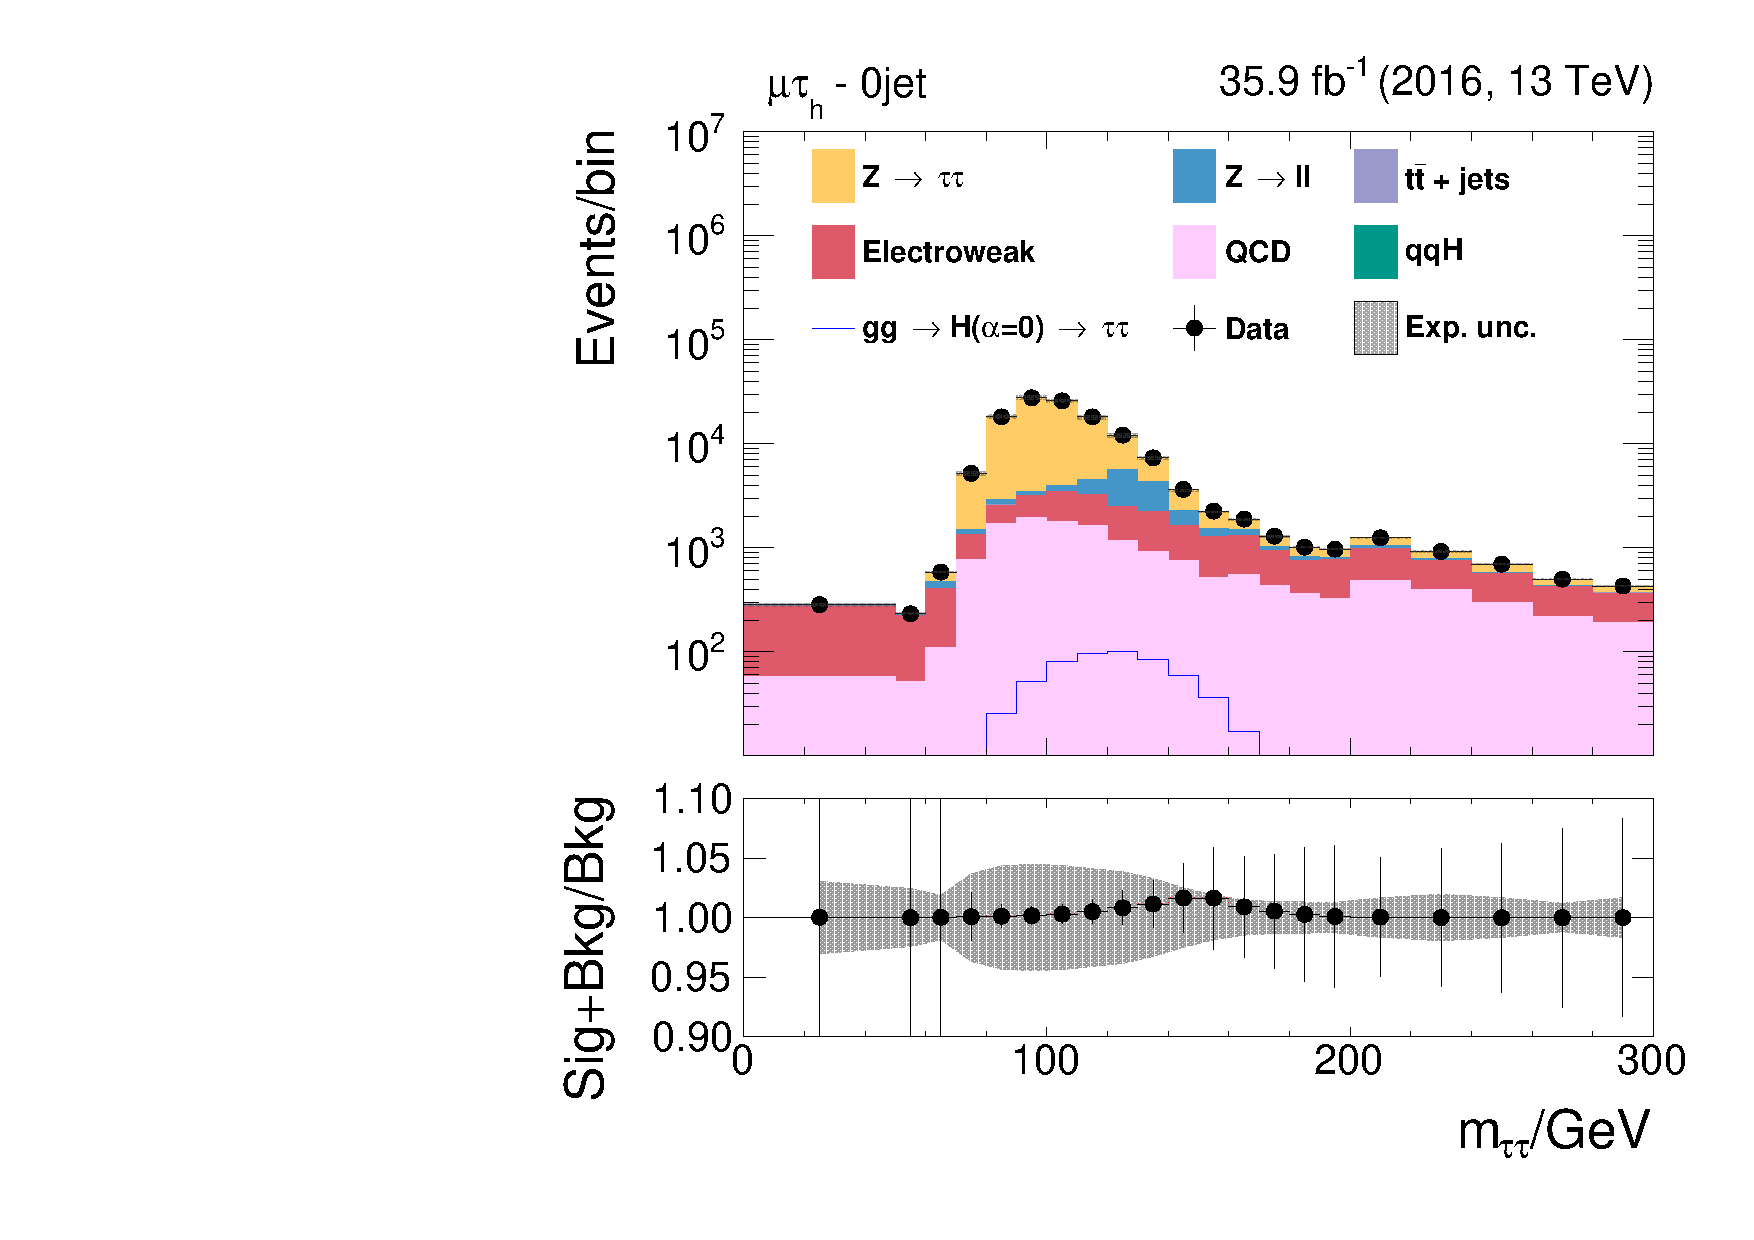
\includegraphics[width=.5\textwidth]{Figures/statana/Postfit_JEC_jdphi/postfit_fit_s_htt_mt_1_13TeV.pdf}\\
        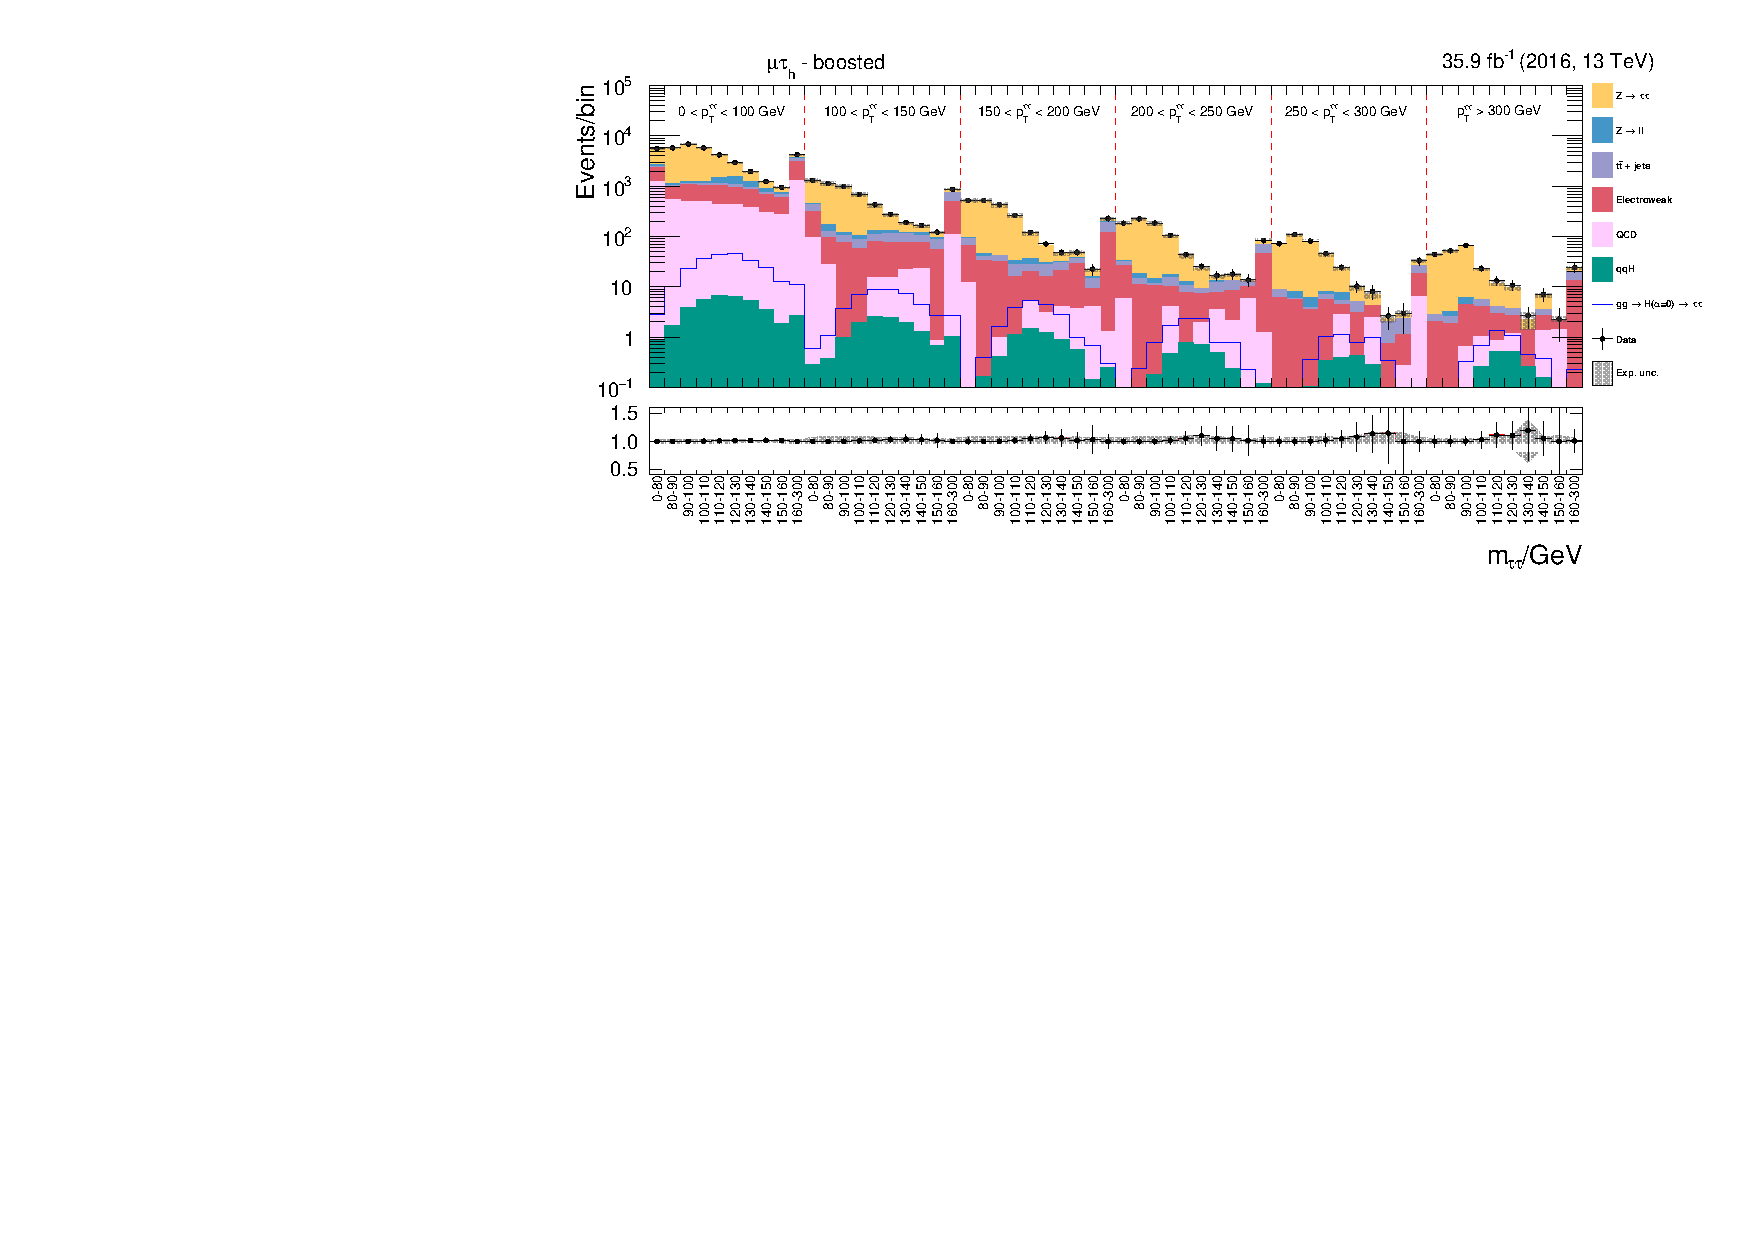
\includegraphics[width=\textwidth]{Figures/statana/Postfit_JEC_jdphi/postfit_fit_s_htt_mt_2_13TeV.pdf}    
    \caption{Postfit distributions of the \textit{0-jet} and \textit{boosted} categories in the \mutau{} channel  using \jdphi{}.}
\end{figure}
\begin{figure}[h!]
    \centering
        \includegraphics[width=\textwidth]{Figures/statana/Postfit_JEC_jdphi/postfit_fit_s_htt_mt_3_13TeV.pdf}\\
        \includegraphics[width=\textwidth]{Figures/statana/Postfit_JEC_jdphi/postfit_fit_s_htt_mt_4_13TeV.pdf}
    \caption{Postfit distributions of the \textit{dijet lowboost} and \textit{dijet boosted} categories in the \mutau{} channel  using \jdphi{}.}
\end{figure}
\clearpage
\begin{figure}[h!]
    \centering
        \includegraphics[width=.5\textwidth]{Figures/statana/Postfit_JEC_jdphi/postfit_fit_s_htt_et_1_13TeV.pdf}\\
        \includegraphics[width=\textwidth]{Figures/statana/Postfit_JEC_jdphi/postfit_fit_s_htt_et_2_13TeV.pdf}
    \caption{Postfit distributions of the \textit{0-jet} and \textit{boosted} categories in the \etau{} channel  using \jdphi{}.}
\end{figure} 
\begin{figure}[h!]
    \centering       
        \includegraphics[width=\textwidth]{Figures/statana/Postfit_JEC_jdphi/postfit_fit_s_htt_et_3_13TeV.pdf}\\
        \includegraphics[width=\textwidth]{Figures/statana/Postfit_JEC_jdphi/postfit_fit_s_htt_et_4_13TeV.pdf}
    \caption{Postfit distributions of the \textit{dijet lowboost} and \textit{dijet boosted} categories in the \etau{} channel  using \jdphi{}.}
\end{figure}
\clearpage
\begin{figure}[h!]
    \centering
        \includegraphics[width=.5\textwidth]{Figures/statana/Postfit_JEC_jdphi/postfit_fit_s_htt_em_1_13TeV.pdf}\\
        \includegraphics[width=\textwidth]{Figures/statana/Postfit_JEC_jdphi/postfit_fit_s_htt_em_2_13TeV.pdf}
    \caption{Postfit distributions of the \textit{0-jet} and \textit{boosted} categories in the \emu{} channel  using \jdphi{}.}
\end{figure}
\begin{figure}[h!]
    \centering
        \includegraphics[width=\textwidth]{Figures/statana/Postfit_JEC_jdphi/postfit_fit_s_htt_em_3_13TeV.pdf}\\
        \includegraphics[width=\textwidth]{Figures/statana/Postfit_JEC_jdphi/postfit_fit_s_htt_em_4_13TeV.pdf}
    \caption{Postfit distributions of the \textit{dijet lowboost} and \textit{dijet boosted} categories in the \emu{} channel  using \jdphi{}.}\label{SUPPLE:SA:postfit_em_2jet}
\end{figure}
\clearpage
